\chapter{Hallazgos y comparación}
\label{cap:hallazgos}

\section{Introducción}
\label{sec:hallazgos:intro}

De las 25 preguntas del catálogo que tienen respuesta con el
instrumental del canal API, 12 se responden en las ocho APIs a la vez.
Con cuatro Datasheets eran 17, y las cinco que caen son las cinco de
Brevo, por dos huecos de su página de precios. Ninguno de sus planes de
pago documenta qué ocurre al superar la cuota, la página de precios niega
que exista precio de exceso y los escalones intermedios de su deslizador
de volumen no tienen precio. Esas cinco preguntas se quedan sin el
sobrecoste o sin el precio del escalón que necesitan. Por API, Resend responde 22, Amazon SES y MailerSend
21, SendGrid, Mailgun y Mailchimp 20, Postmark 18 y Brevo 16. De las 18
de Postmark, 7 dependen de un \textit{rate} que el proveedor no publica
y que la Datasheet adopta en ámbar desde la cabecera medida por sondeo.
Este capítulo lee las Datasheets del catálogo con dos preguntas de
investigación delante.

La primera es RQ3: cómo se relacionan los límites de uso y los
\textit{rates} en las APIs de correo, y qué implicaciones tiene esa
relación para el consumidor. Su respuesta es la contribución C-03: cómo
se relacionan ambos límites en el correo y qué se sigue de ello para
quien consume la API. La segunda es RQ4: cómo pueden compararse las APIs
de forma sistemática para responder a preguntas de decisión que mezclan
requisitos funcionales y no funcionales. Su respuesta es la contribución
C-04: un catálogo de preguntas de decisión con el procedimiento para
resolverlas sobre las Datasheets.

El capítulo no responde a RQ2. Los elementos que el esquema ACM2YAML no soporta y que
dejó la construcción del catálogo aparecen aquí solo por su id, cuando
un hecho depende de ellos, y se tratan en el
Capítulo~\ref{cap:evolucion}. Los identificadores que usa el capítulo
son estos. F-nn es un elemento que el esquema no soporta, y va en el
inventario que abre el Capítulo~\ref{cap:evolucion}. O-nn es una observación
que no es carencia del esquema, y el mismo capítulo le dedica una sección.
P-nn es una propuesta de extensión del esquema
del Capítulo~\ref{cap:evolucion}. Y Q1 a Q10 son las operaciones de
PRIME4API \citep{gavira2026tfm}, que la
Sección~\ref{sec:hallazgos:limites-rates} nombra por su número.

Los hechos proceden de las Datasheets construidas con el método del
Capítulo~\ref{cap:catalogo}: documentación pública, panel con cuenta
propia y sondeo contra la API, con semáforo y \textit{provenance} por
campo. En este capítulo «hechos» son los valores de la Datasheet y los de
su registro de fuentes y evidencias, que guarda lo que ningún campo del
esquema admite. Las Datasheets no se reproducen en la memoria, y se
conservan con sus fuentes y evidencias en el repositorio de datos que
acompaña al trabajo.

A la fecha de este capítulo hay ocho Datasheets construidas y sondeadas.
Postmark \citep{postmarkpricing} fue el piloto, y después se
construyeron Resend \citep{resendpricing}, SendGrid
\citep{sendgridpricing}, MailerSend \citep{mailersendpricing}, Brevo
\citep{brevopricing}, Amazon SES \citep{sespricing}, Mailgun
\citep{mailgunpricing} y Mailchimp Transactional
\citep{mailchimppricing}. Todo recuento y todo porcentaje de este
capítulo se refiere a esas ocho. Tres sondeos midieron un estado de la
suscripción y no el plan: el de MailerSend sobre una cuenta Sandbox sin
aprobar, el de SES sobre el entorno de pruebas y el de Mailchimp sobre
una cuenta de prueba. El Apartado~\ref{subsec:evolucion:p06} define el estado de la suscripción y lo separa de la reputación. Ningún valor de plan de esas tres Datasheets
cambia de semáforo por medición.
Las cifras llevan punto de miles y coma decimal, también los precios.
Solo el literal del proveedor entre comillas conserva su forma.

El capítulo se organiza del siguiente modo. En primer lugar, la
Sección~\ref{sec:hallazgos:apis} recoge lo que revela cada API con el
mismo guion de cuatro bloques (documentación, panel, sondeo y lo que se
aprende del proveedor). A continuación, la
Sección~\ref{sec:hallazgos:limites-rates} calcula sobre las ocho APIs la
relación entre límites de uso y \textit{rates}, que es la respuesta a
RQ3.
Después, la Sección~\ref{sec:hallazgos:catalogo-pi} presenta el catálogo
de preguntas de Pricing Intelligence y la
Sección~\ref{sec:hallazgos:comparacion} lo ejercita sobre las ocho
Datasheets, que es la respuesta a RQ4. Por último, la
Sección~\ref{sec:hallazgos:conclusiones} resume las dos respuestas junto
con lo que queda pendiente.

\section{Lo que revela cada API}
\label{sec:hallazgos:apis}

Cada subsección sigue el formato que fijó el piloto en la
Sección~\ref{sec:propuesta:piloto}, reordenado en cuatro bloques por
fuente, porque cada API se distingue por lo que cada fuente añade sobre la
anterior. Una apertura anuncia los hallazgos de la API y el estado de la
suscripción que acota lo medido. El primer bloque recoge lo que la documentación
pública declara sobre planes, cuotas, \textit{rates}, topes por petición y
sobrecoste. El segundo recoge lo que añadió el panel con cuenta propia,
segundo peldaño de la escalera de validación de la
Sección~\ref{sec:propuesta:validacion}. El tercero recoge lo que añadió el
sondeo, el tercer peldaño: peticiones reales contra la API, con sus códigos
de respuesta y sus cabeceras. El cuarto recoge lo que se aprende del proveedor,
hallazgo a hallazgo, y cierra con el límite de la lectura. La respuesta de
PRIME4API sobre la Datasheet, si la hay, va en el tercer bloque o en el
cuarto, junto al hallazgo que sostiene. Importa sobre
todo lo que la documentación no dice y el panel o la API sí. Importan
también las discrepancias entre fuentes y lo que el proveedor no publica.
Entre fuentes se distinguen tres fenómenos, siempre con el mismo nombre.
Hay contradicción si dos fuentes dan valores o condiciones incompatibles
para el mismo atributo, ausencia si un canal no publica el límite y
diferencia de canal si dos canales describen superficies distintas del
servicio.
Cuando la contradicción enfrenta a la página de precios con otra fuente, se resuelve a favor de la página y el otro valor se lee como incoherencia del \textit{pricing}.
Los elementos no soportados se nombran por su id. F-01 a F-22
se tratan en el Capítulo~\ref{cap:evolucion}, con las observaciones O-nn y
las propuestas P-nn, y las posteriores, desde F-23, se definen aquí la
primera vez que aparecen. Cada cifra lleva su fuente, y la prosa dice
cuándo el campo está en ámbar o en rojo.

Dos reglas gobiernan la lectura de los sondeos. Se aplican igual a las
ocho APIs. La primera dice qué valida un sondeo sin envío real. Un
sondeo con token de pruebas o en modo \textit{sandbox} valida los topes
por petición que la API comprueba al recibir la petición, como los
destinatarios o el tamaño del mensaje. No todas lo hacen: el lote de
MailerSend valida cada correo después de aceptar la petición, y Mailchimp
encola por encima de diez destinatarios sin nombrar ningún tope.
Ningún sondeo de este tipo valida la cuota consumida ni el caudal. Cuando la petición se rechaza por validación
con un token real, como en los sondeos de caudal de Postmark, MailerSend y
Brevo, el contador de caudal sí descuenta, y en MailerSend también la
cuota diaria de peticiones. La segunda dice cuándo un valor observado entra
en la Datasheet. Entra cuando el sondeo se diseñó para medirlo y es
inocuo. Una cabecera aparecida en un sondeo de otro propósito, si
difiere de lo publicado, se anota como valor observado pendiente, y
adoptarla exige un sondeo de caudal. Por la misma regla, un valor publicado va en verde si nada lo
contradice, aunque no se haya medido.
Si el valor lo publica la página de precios y el sondeo mide menos, se mantiene el valor publicado y la medida queda como incoherencia del \textit{pricing}.

Las ocho APIs se presentan en el orden en que se construyeron, el de la
Sección~\ref{sec:hallazgos:intro}.

\subsection{Postmark}
\label{subsec:hallazgos:postmark}

Postmark \citep{postmarkpricing,postmarkapi} deja cuatro hallazgos que se
suman a la lectura del piloto
(Sección~\ref{sec:propuesta:piloto} y Tabla~\ref{tab:lecturapostmark}, con
los semáforos anteriores a septiembre). El primero es de capacidad: la API
declara en cabecera un \textit{rate} de 5.000 peticiones que la
documentación no publica. El segundo es de topes por petición: el lote de
500 mensajes queda verificado y pasa de ámbar a verde. En el envío masivo el proveedor no pone tope de mensajes:
lo que acota es la carga, en megabytes. El tercero es de esquema: la
documentación y el panel muestran tres restricciones que v0.3 no recoge,
una sobre el relé SMTP y dos sobre la administración de la cuenta. El
cuarto es de validez, porque ninguna petición con token real llegó a enviar
un correo.

La cuenta propia está en el \textit{tier} gratuito y en modo de prueba. En
ese modo solo se pueden enviar 100 correos, y solo a dominios verificados.
Está además pendiente de aprobación. Mientras lo esté, el proveedor rechaza
con ErrorCode 412 cada mensaje dirigido a un dominio distinto del
remitente: «all recipient addresses must share the same domain as the
`From' address». Cada mensaje de los sondeos con token real iba a un
dominio no verificado o excedía el tope de destinatarios, y por eso ninguno
salió. No se leyó un contador de cuota antes y después, así que el gasto
nulo de cuota de correos se infiere del código de rechazo de cada mensaje.
Cambiar de plan exige enviar antes una solicitud de aprobación, y lo
observado es solo el \textit{tier} gratuito.

\paragraph{Qué dice la documentación.} El \textit{rate} de la API REST no
está publicado. La referencia describe el error 429, «Rate Limit
Exceeded», sin umbral numérico ni ámbito \citep{postmarkapi}.

Los topes por petición que publica la referencia están en la
Tabla~\ref{tab:hallazgos:postmark:topes}, junto a lo que midió el sondeo.
El proveedor mide el tamaño del correo «after it has been base64 encoded»
\citep{postmarkapi}, y la Datasheet deja las cotas en megabytes en el
\textit{provenance}. Lo que v0.3 no puede decir es que una cota en megabytes acote el máximo en
correos, que en el envío masivo queda vacío (F-06).

El único límite de concurrencia que publica Postmark es de diez conexiones
simultáneas por IP, y es una recomendación para el relé SMTP, un canal
distinto de la API REST. El proveedor avisa de que «We do not have any
systems in place to enforce these limits» y califica esos límites de
«somewhat arbitrary, and informal» (F-04). Para la API REST no publica
ninguno, una ausencia que el fichero registra en \texttt{not\_found}.

\paragraph{Qué añadió el panel.} El panel aporta dos de las restricciones
que v0.3 no recoge, y una es el tope de servidores. En la cuenta gratuita
fija en diez los servidores que se pueden crear y pide subir de
\textit{tier} para crear más: «Upgrade your Tier to create more servers».
La lista de \textit{tiers} del mismo panel no da cifra para el gratuito y
da cinco servidores a Basic, diez a Pro e ilimitados a Platform. Ninguna de
las dos pantallas explica que la cuenta gratuita admita más servidores que
Basic. Las cuotas de v0.3 llevan periodo y se gastan, y un servidor se
tiene o no se tiene, así que el tope queda sin campo en el fichero (F-11).

La otra es la gestión de credenciales: en lo que Postmark publica, generar
o borrar el token de un servidor ya creado solo tiene canal en el panel. La
pestaña de tokens del servidor ofrece «Generate another token» y «Delete»,
que se observaron sin pulsar. La referencia de la API no publica ninguna
operación equivalente, y lo único programable es \texttt{POST /servers},
que crea un servidor nuevo con sus tokens. El fichero solo declara el canal
del documento entero, \texttt{type: api\_first}, y no tiene campo para
decir que una operación suelta se hace desde la web (F-22).

Los complementos quedan fuera de la Datasheet por alcance: el esquema
los deriva al canal web, que este trabajo no modela, y sus precios van al
\textit{provenance} (F-07, Apartado~\ref{subsec:evolucion:f07}). La
página de precios publica el de tres de ellos con la fórmula «Starts at»
\citep{postmarkpricing}.

\paragraph{Qué añadió el sondeo.} La cabecera da la cifra que la
documentación no publica. En los tres sondeos con token real, las
respuestas de los cuatro endpoints de envío probados traen
\texttt{ratelimit-limit: 5000}, sea el código 200 o 422. Las que se
archivaron completas traen cinco cabeceras de \textit{rate} que la
documentación no menciona, entre ellas
\texttt{x-ratelimit-limit-second: 5000} y \texttt{ratelimit-reset: 1}. Que
el límite sea por segundo es inferencia de esos nombres, no un literal del
proveedor. La primera respuesta archivada con esas cabeceras es de un
sondeo diseñado para contar destinatarios. Por la segunda regla de esta
sección, el valor no entró en el campo hasta el sondeo de caudal.

El sondeo de caudal no alcanzó el 429, pero descarta una lectura del
contador. Envió 200 peticiones a \texttt{/email} con token real, 25 en
paralelo, en 4,57 segundos, y todas se rechazaron con ErrorCode 412. Las
respuestas caen en cinco segundos del reloj del servidor, y en cada uno el
contador \texttt{ratelimit-remaining} marca 4.999 entre cuatro y ocho
veces. El mínimo de todo el sondeo es 4.986, en el segundo con 48
respuestas. Un solo contador que descontase cada petición al responder
marcaría 4.999 únicamente en la primera respuesta de cada ventana, y un
segundo del reloj toca como mucho dos ventanas de un segundo. Ese contador
no marcaría 4.999 más de dos veces por segundo, y en el segundo de 48
respuestas habría bajado a 4.976 o menos. Lo observado es compatible con
varios contadores en paralelo o con uno que no se actualiza al instante, y
el sondeo no distingue entre esas dos explicaciones.
Si la cabecera describe el límite, alcanzar el 429 exigiría al menos 5.000
peticiones en un segundo, más de lo que admite el sondeo ligero del tercer
peldaño (Sección~\ref{sec:propuesta:validacion}).

El sondeo de lote sirve de control sobre qué descuenta el contador: la
respuesta a una petición con 500 mensajes marca 4.999, lo mismo que la de
una petición con uno. Si el contador descontase los mensajes al responder,
como descuenta la propia petición, habría marcado 4.500 o menos. El
resultado vale para mensajes rechazados, y el sondeo no observa si un
mensaje enviado descuenta aparte. Es coherente con la unidad
\texttt{requests} en la que el fichero declara el \textit{rate}.

En \texttt{max\_power} el valor figura en ámbar, como 5.000 peticiones por
segundo, y pasaría a verde solo si un sondeo alcanzase el 429. El fichero
lo referencia desde los cuatro planes por decisión de modelado, la de un
solo \textit{rate} no condicionado al plan. Esa decisión extrapola a los
planes de pago un valor observado solo en la cuenta gratuita, y ninguna
cabecera nombra el plan al que pertenece. Algunas respuestas traen además
\texttt{x-postmark-account} y \texttt{x-postmark-server}, y ninguna de las
dos cabeceras dice si el límite se aplica a la cuenta o al servidor.

\begin{table}[H]
\centering
\scriptsize
\setlength{\tabcolsep}{3pt}
\renewcommand{\arraystretch}{1.15}
\begin{tabular}{|p{0.19\textwidth}|p{0.27\textwidth}|p{0.29\textwidth}|p{0.12\textwidth}|}
\hline
\raggedright \textbf{Endpoint} & \raggedright \textbf{Referencia} & \raggedright \textbf{Sondeo} & \raggedright \textbf{Datasheet} \tabularnewline
\hline
\raggedright \texttt{/email} & \raggedright «Max 50» en cada campo (\texttt{To}, \texttt{Cc} y \texttt{Bcc}). 10~MB por mensaje & \raggedright Token de pruebas. 50 en total, aceptados en dos repartos. 51 en total, 422 en tres repartos. 150 en total, 422 & \raggedright 50 en total~\semverde \tabularnewline
\hline
\raggedright \texttt{/email/\allowbreak withTemplate} & \raggedright --- & \raggedright Token real. 51 en \texttt{To}, 422 con ErrorCode 300 & \raggedright 50 en total~\semverde \tabularnewline
\hline
\raggedright \texttt{/email/batch} y \texttt{/email/\allowbreak batchWithTemplates} & \raggedright 500 mensajes por llamada. 50~MB de carga (solo \texttt{/email/batch}) & \raggedright Token real. 500 mensajes, lote aceptado con 200. 501, 422 con ErrorCode 410 & \raggedright 500~\semverde \tabularnewline
\hline
\raggedright \texttt{/email/bulk} & \raggedright Sin tope de mensajes. Destinatarios «as many recipients as you need». 50~MB de carga. «Max 50» destinatarios por mensaje & \raggedright 403 con el token de pruebas, sin medir & \raggedright vacío~\semrojo \tabularnewline
\hline
\end{tabular}
\caption{Postmark: topes por petición de los cinco endpoints de envío según la
referencia \citep{postmarkapi}, el sondeo y la Datasheet. El guion marca ausencia: la
referencia no publica un tope propio para el envío con plantilla. La fila de \texttt{/email}
repite el sondeo del piloto (Sección~\ref{sec:propuesta:piloto}) para compararla con la de
plantilla. En esa fila la referencia da 50 por campo y el sondeo mide 50 en total, que es lo
que adopta la Datasheet. La última columna es el máximo del
\texttt{workload}, que el fichero declara en la unidad \texttt{emails} en los cinco
endpoints, y las cotas en megabytes quedan en el \textit{provenance} (F-06).}
\label{tab:hallazgos:postmark:topes}
\end{table}

Con token real, \texttt{/email/\allowbreak withTemplate} rechaza lo mismo
que el piloto rechazó en \texttt{/email}. Con 51 destinatarios, todos en
\texttt{To}, devuelve 422 y el mismo mensaje, «Maximum of 50 recipients
allowed per email message». El reparto no se varió, y el tope en total se
apoya aquí en el literal del error, que cuenta por mensaje. Los dos
endpoints de lote responden 200 a una petición de 500 mensajes y
rechazan la de 501 con «You may only send up to 500 messages in a single
batched request». Ese par de medidas fija el tope exacto. El envío masivo
quedó sin medir: el único intento usó el token de pruebas, que «may only be
used on the /email endpoint», y devolvió 403.

\paragraph{Qué se aprende del proveedor.} Postmark es el caso de F-01 con
el valor a la vista: un \textit{rate} sin publicar que la API declara en
cabecera. Mientras el bloque \texttt{max\_power} no declaró ningún caudal, PRIME4API
respondió como si no hubiera límite
(Sección~\ref{sec:hallazgos:limites-rates}). P-04 propone una marca que
separe «límite no publicado» de «sin límite»
(Apartado~\ref{subsec:evolucion:p04}). Con el valor en ámbar el fichero
declara a la vez la cifra observada, en \texttt{max\_power}, y que el
proveedor no la publica, en \texttt{not\_found}.

Los topes por petición tocan tres propuestas del
Capítulo~\ref{cap:evolucion}. En el fichero la unidad \texttt{emails}
cuenta destinatarios en \texttt{/email} y mensajes en el lote, y el
proveedor no publica cómo se contabiliza un lote cuyos mensajes llevan sus
propios destinatarios. Es F-03, el elemento no soportado que aborda P-02
(Apartado~\ref{subsec:evolucion:p02}). El envío masivo acota la carga en
megabytes y no en mensajes, que es F-06 y el caso de P-03 en ese mismo
apartado. Su campo de mensajes queda además presente y vacío, el hueco que
describe P-04, y con él fallan las operaciones de cálculo del motor.

Ninguna de las tres restricciones que v0.3 no recoge produce propuesta en
el Capítulo~\ref{cap:evolucion}.
La de SMTP es una recomendación que el proveedor dice no
hacer cumplir (F-04), y la Sección~\ref{sec:evolucion:fuera} la discute sin
forma fijada. La de servidores es un recurso
que se tiene y no se consume (F-11). La de credenciales es una operación
cuyo único canal publicado es el panel (F-22). Las dos quedan promovidas,
con una forma esbozada en la Tabla~\ref{tab:sinforma}.

El límite de esta lectura es el estado de la suscripción descrito al principio.
El contador de \textit{rate} solo se ha leído con mensajes rechazados, y
el 429 no se ha alcanzado. Tampoco se han
observado el precio de cada volumen contratado en Pro y Platform ni el
reprecio al cambiar de \textit{tier}, que el panel no muestra con la
cuenta sin aprobar. Y
queda abierto si la cuota descuenta por destinatario o por mensaje.

\subsection{Resend}
\label{subsec:hallazgos:resend}

Resend \citep{resendpricing,resenddocs} deja cuatro hallazgos, de capacidad, precio, plan
negociado y fuentes. La documentación cuenta la cuota por destinatario, y
el sondeo fija el tope de 50 destinatarios sobre la suma de \texttt{to} y \texttt{cc}.
Pro y Scale se venden por volúmenes contratados, y una cuota de v0.3 admite solo uno.
Enterprise no tiene precio, volumen ni \textit{rate} publicados, y mientras está en la
Datasheet el motor no devuelve ningún plan cuando la consulta los compara todos. Resend es la única de las ocho APIs cuyo
\textit{rate} coincide en documentación, panel y cabecera de respuesta.

Lo medido sale de una cuenta Free sin dominio verificado, que solo puede enviar a la
propia dirección. Los valores de los planes de pago se conocen únicamente por la documentación.

\paragraph{Qué dice la documentación.} La unidad de consumo es el destinatario:
«Multiple To, CC, or BCC recipients count as separate emails». En \texttt{/emails} solo el
campo \texttt{to} declara tope, «Max 50», sin aclarar si suma \texttt{cc} y
\texttt{bcc}. El lote admite 100 mensajes con ese tope en cada \texttt{to}. De los dos
literales se infiere que el consumo de una llamada puede llegar al producto de mensajes
por destinatarios (F-03). Los adjuntos se acotan en bytes, 40 MB tras la codificación
base64 (F-06).

La recepción también gasta cuota: «Both sent and received emails count towards these
quotas» (F-12). Un correo que llega por encima de la cuota se recibe, pero su contenido no
se puede recuperar.

Pro se contrata en dos volúmenes y Scale en seis (F-02). En Scale el sobrecoste baja con
cada volumen, y en Pro no cambia. Cada cuota de v0.3 admite un volumen y un sobrecoste,
así que la Datasheet guarda el primero de cada plan (Tabla~\ref{tab:hallazgos:resend}).

El \textit{rate} por defecto es «10 requests per second per team»
\citep{resenddocs}, y no se documenta si varía por plan. Como se publica por
equipo y ningún plan publica otro, la Datasheet aplica ese valor a Pro y Scale. La
página de precios pone «Custom» en el precio, el volumen y el sobrecoste de Enterprise,
y lista «Enterprise rate limits» sin cifra (F-01). La Datasheet copia \texttt{custom} y
deja vacío su \textit{rate}, en rojo.

\begin{table}[H]
\centering
\footnotesize
\setlength{\tabcolsep}{3pt}
\begin{tabular}{|l|r|r|r|c|}
\hline
\textbf{Plan} & \textbf{Volumen} & \textbf{Precio} & \textbf{Sobrecoste} & \textbf{\textit{Rate}} \\
 & (correos/mes) & (USD/mes) & (USD/1.000) & (req/s) \\
\hline
Free & 3.000 y 100/día~\semverde & 0~\semverde & no disponible & 10~\semverde \\
\hline
Pro & 50.000~\semverde & 20~\semverde & 0,90~\semverde & 10 (def.)~\semverde \\
 & 100.000 & 35 & 0,90 & \\
\hline
Scale & 100.000~\semverde & 90~\semverde & 0,90~\semverde & 10 (def.)~\semverde \\
 & 200.000 & 160 & 0,80 & \\
 & 500.000 & 350 & 0,70 & \\
 & 1.000.000 & 650 & 0,65 & \\
 & 1.500.000 & 825 & 0,52 & \\
 & 2.500.000 & 1.150 & 0,46 & \\
\hline
Enterprise & custom~\semverde & custom~\semverde & custom & no publicado~\semrojo \\
\hline
\end{tabular}
\caption{Resend: volúmenes contratados por plan \citep{resendpricing}. Las
filas con semáforo son las que la Datasheet serializa, el primer volumen de
cada plan. Las demás quedan en el \textit{provenance} (F-02). El semáforo es el de la Sección~\ref{sec:propuesta:trazabilidad}, y «custom» es el literal del proveedor. Las ventanas de la cuota mensual y de la diaria están en ámbar
(\semambar{}). En Pro y Scale, «def.» marca el \textit{rate} por defecto de la documentación. Free no
admite sobrecoste. El tope de 50 destinatarios por petición no tiene columna
porque la documentación no lo ata al plan, y se midió en la cuenta Free.}
\label{tab:hallazgos:resend}
\end{table}

\paragraph{Qué añadió el panel.} Los contadores «Monthly limit 0 / 3000» y «Daily limit 0 /
100» tienen cada uno una fila de envío y otra de recepción (F-12), y el panel repite «Rate limit 10 req/s».

El sobrecoste es opcional (F-13): en el panel es un interruptor apagado, marcado «Paid
feature», cuyo texto empieza por «When enabled». El campo \texttt{overage\_cost} no puede
declarar que el sobrecoste existe solo si el cliente lo activa.

La suscripción de marketing que muestra la cuenta se limita por contactos, así que queda
fuera por alcance (F-10). Tampoco entran los complementos, que el esquema deriva al
canal web (F-07).

\paragraph{Qué añadió el sondeo.} El tope de destinatarios es de la petición y no de cada
campo. Todas las entradas llevaban la propia dirección. Con 51 en \texttt{to}, la API
devolvió 422 con «Field \texttt{to} has a maximum of 50 items». Con 26 en \texttt{to} y
25 en \texttt{cc}, que un tope por campo habría aceptado, devolvió otro 422 con «The total
number of recipients cannot exceed 50». Con 25 y 25 devolvió 200. Postmark
tiene el mismo tope conjunto (Apartado~\ref{subsec:hallazgos:postmark}). El campo
\texttt{bcc} no se probó, así que lo medido suma solo \texttt{to} y \texttt{cc}.

La cabecera repite el \textit{rate} de la documentación y del panel: las cuatro respuestas
traían \texttt{ratelimit-limit: 10}. El corte no se provocó: las peticiones iban
separadas entre dos y tres segundos, y en todas quedaron nueve disponibles.

Ante una dirección repetida la validación del tope contó cada entrada y la cuota no. La
documentación no dice cómo cuenta una dirección repetida. Se aceptaron dos envíos: uno iba
a un destinatario y el otro llevaba la propia dirección 25 veces en \texttt{to} y 25 en
\texttt{cc}. El panel pasó de 0 a «Daily limit 2 / 100». Contar cada entrada habría dado
51. Contar por mensaje o fundir las repeticiones da 2, y el experimento no distingue ambas
reglas. En SES una dirección repetida en \texttt{to} y en \texttt{cc} contó dos veces
(Apartado~\ref{subsec:hallazgos:ses}).

La cabecera \texttt{x-resend-daily-quota} marcó el consumo previo a cada envío aceptado: 0
en el primero y 1 en el segundo. La documentación la describe como el consumo usado, sin
decir si incluye la petición en curso. Con solo dos lecturas no se sabe si la cabecera se calcula antes de contar el envío o si el contador se actualiza tras responder.

Las dos ventanas de la cuota siguen en ámbar, porque el panel no muestra fecha de
reposición. Para la diaria la documentación solo dice «wait until 24 hours have passed», y ninguna
lectura del contador fija cuándo empiezan esas 24 horas.

PRIME4API falla sobre la Datasheet completa cuando la consulta
recorre todos los planes. Pedida la
suscripción más barata para 40.000 correos, devuelve 500 con \texttt{float() argument must
be a string or a real number, not 'NoneType'}. El único campo vacío del fichero es el
\textit{rate} de Enterprise. Sin ese plan, la misma consulta responde Pro, a 20 USD. El
error apunta al campo vacío, pero retirar el plan retira también sus cadenas
\texttt{custom} de precio y volumen. Esas cadenas hacen fallar la Datasheet de SendGrid ante la misma consulta, con otro error, y el 500 de Resend puede venir del campo vacío o de ellas.

\paragraph{Qué se aprende del proveedor.} Según la documentación, una llamada a Resend
consume tantas unidades como destinatarios lleve, y de ahí se infiere que en el lote ese
consumo puede llegar a multiplicarse por el número de mensajes. El \texttt{workload} de v0.3 solo admite un
máximo escalar, así que el factor queda en una descripción (F-03, P-02,
Apartado~\ref{subsec:evolucion:p02}). Tampoco hay dónde declarar que el tope cuenta las
direcciones repetidas y la cuota no.

Los volúmenes contratados son un caso de P-01 (Apartado~\ref{subsec:evolucion:p01}),
porque el fichero guarda uno por plan, y la Sección~\ref{sec:hallazgos:comparacion} mide
cuánto se desvía el motor sin los demás.

El \textit{rate} vacío de Enterprise es un caso de P-04 (Apartado~\ref{subsec:evolucion:p04}),
porque v0.3 no marca un valor que existe sin publicarse. Su \texttt{custom} de precio y
volumen es un caso de P-05 (Apartado~\ref{subsec:evolucion:p05}). Que un solo plan
negociado impida calcular los demás es lo que la propuesta de P-05 para el motor quiere
evitar.

Resend es uno de los tres contraejemplos del desajuste entre el \textit{rate} publicado y
el observado (Sección~\ref{sec:hallazgos:limites-rates}). Lo que coincide en documentación, panel y cabecera es el valor declarado en la cuenta Free, no un corte medido. Sin dominio verificado, la cuenta no puede enviar a destinatarios distintos, y el sondeo dejó sin medir el corte del \textit{rate} y el campo \texttt{bcc}.

El repositorio de la guía \citep{apisconsumptionmodel}, del 2026-02-24,
modela Resend con 2 peticiones por segundo, y la documentación del 2026-08-05 publica
10. Sin la página de febrero, la diferencia no se puede atribuir ni a un cambio de la
oferta, que sería un caso de F-09, ni a la lectura de entonces.

\subsection{SendGrid}
\label{subsec:hallazgos:sendgrid}

SendGrid \citep{sendgridpricing,sendgriddocs} deja cuatro hallazgos. En el
precio, el envío mensual de Essentials y Pro tiene un techo de
diez veces el volumen del plan, sobrecoste incluido, y v0.3 declara el
sobrecoste como un precio unitario sin máximo. En la vigencia, la prueba
gratuita dura 60 días y después se detiene el envío, pero el único dato
temporal de un plan en v0.3 es su periodo de facturación, y no hay campo de
vigencia. En las fuentes, el modelado necesita dos datos que solo aparecen
fuera de las páginas de precios y de límites: el caudal de envío y el techo
del sobrecoste. En la capacidad por petición, el proveedor publica el tope total
de destinatarios y el sondeo lo verifica, así que el tope escalar de v0.3
basta. El relé SMTP tiene en cambio topes propios que el esquema no sabe
declarar.

La cuenta observada está en la prueba gratuita, con un tope duro de 100
correos al día. Los envíos de los sondeos usaron el modo \textit{sandbox}, que
valida la petición sin entregarla ni consumir créditos. Por la primera regla
de esta sección, miden topes por petición. Las lecturas de otros endpoints sí fueron
llamadas reales con la clave de la cuenta. La Datasheet modela solo el Email
API, porque el proveedor cuenta aparte los envíos de Marketing Campaigns
(F-10).

\paragraph{Qué dice la documentación.} El precio depende del volumen
contratado: Essentials se contrata en dos volúmenes y Pro en cinco, cada uno
con su precio y su sobrecoste (F-02). La Datasheet declara un plan por
\textit{tier} en su volumen mínimo, la convención fijada en la
Sección~\ref{sec:propuesta:piloto}, y la Tabla~\ref{tab:hallazgos:sendgrid}
recoge todos los volúmenes.

\begin{table}[H]
\centering
\footnotesize
\setlength{\tabcolsep}{4pt}
\begin{tabular}{|l|r|r|r|r|c|}
\hline
\textbf{Plan} & \textbf{Precio} & \textbf{Volumen} & \textbf{Sobrecoste} &
\textbf{Sobrecoste} & \textbf{Techo} \\
 & & \textbf{incluido} & \textbf{web} & \textbf{panel} & \textbf{mensual} \\
 & (USD/mes) & (correos/mes) & (USD/correo) & (USD/correo) & \\
\hline
Free Trial & 0,00~\semverde & 100 al día~\semverde & no aplica & no aplica & no aplica \\
\hline
Essentials 50K & 19,95~\semverde & 50.000~\semverde & 0,0013~\semverde & 0,00133 & 10X (500.000) \\
\hline
Essentials 100K & 34,95 & 100.000 & 0,0009 & 0,0009 & 10X \\
\hline
Pro 100K & 89,95~\semverde & 100.000~\semverde & 0,0011~\semverde & 0,0011 & 10X \\
\hline
Pro 300K & 249,00 & 300.000 & 0,0009 & 0,00091 & 10X \\
\hline
Pro 700K & 499,00 & 700.000 & 0,0008 & 0,00078 & 10X \\
\hline
Pro 1.5M & 799,00 & 1.500.000 & 0,0006 & 0,00059 & 10X \\
\hline
Pro 2.5M & 1.099,00 & 2.500.000 & 0,0005 & 0,00047 & 10X \\
\hline
Premier & custom~\semverde & custom~\semverde & custom & --- & --- \\
\hline
\end{tabular}
\caption{SendGrid: precio por volumen contratado \citep{sendgridpricing}. Precio y
volumen salen de la página de precios y coinciden con el panel. El sobrecoste va en dos
columnas porque el panel lo da con más decimales que la web. A la Datasheet llega el de la
web, y el del panel se registra como incoherencia del \textit{pricing}. El semáforo marca los valores
que llegan a la Datasheet, que declara un plan por \textit{tier} en su volumen mínimo
(F-02). La ventana mensual de Premier es el único campo en ámbar del fichero, porque
ninguna fuente consultada la da para ese plan. El guion indica que la fuente no da el
dato, y «no aplica», que la prueba gratuita no tiene sobrecoste.}
\label{tab:hallazgos:sendgrid}
\end{table}

Desde el 26 de marzo de 2026 el sobrecoste tiene techo: el envío mensual de
Essentials y Pro queda en «10X times the plan», que en Essentials 50K son
500.000 al mes, sobrecoste incluido. El literal cuenta «requests», y el mismo
artículo las define como correos procesados más descartados, «Requests =
Processed + Dropped». De las fuentes consultadas, el techo solo aparece en ese
artículo, que resuelve el error «Maximum Credits Exceeded», y ni la página de
precios ni el artículo de sobrecostes lo mencionan (F-16). El sobrecoste
depende además del canal de contratación: si la cuenta se creó a través de
Heroku o Google Cloud, «your subscription does not allow for overages» (F-13).

La prueba gratuita tiene fecha de fin. Se anuncia a «\$0/mo for 60 days», y al
terminar «email send will stop» salvo que antes se elija un plan del Email API
(F-14). Mientras dura es un tope duro, «You can’t exceed these limitations».
Dar de baja un plan de pago lleva al mismo punto: a final de mes el plan pasa
a «end of trial», sin envío, y no vuelve a ningún plan gratuito.

La FAQ de la página de precios describe un plan gratuito sin mencionar los 60
días, «100 emails per day on our free SMTP plan». El registro de cambios del
27 de mayo de 2025 anuncia la retirada de los planes gratuitos. La Datasheet modela la
prueba de 60 días porque es el plan con el que el panel abrió la cuenta el
2026-09-06. Un modelado que partiera solo de la FAQ declararía un plan
gratuito sin fecha de fin, y el fichero no tiene dónde decir qué parte de una
fuente sigue vigente (F-09).

Solo una FAQ de \texttt{/v3/mail/send} cifra el caudal de envío: «up to
10,000 requests per second». No lo ata a ningún plan ni dice su ámbito, si se
aplica por cuenta, por clave o por subusuario. La página de \textit{rate
limits} no menciona ese endpoint, y sus dos cifras, 500 y 150, salen de
respuestas de ejemplo que no coinciden entre sí. La duración del «refresh
period» tampoco se publica (F-01). La Datasheet copia los 10.000 a los cuatro
planes en verde documental, por la segunda regla de esta sección.

El tope de destinatarios cubre la petición entera: «no more than 1,000» entre
\texttt{to}, \texttt{cc} y \texttt{bcc}, sumados todos los sobres. Un sobre es
un objeto \texttt{personalizations} con sus propios destinatarios, y una
petición admite como mucho 1.000 sobres. Por el literal de la página de precios, cada
destinatario descuenta un crédito, «one email to one recipient», de modo que
una petición llena gasta 1.000 correos de la cuota. Con el total publicado
basta el tope escalar de v0.3, \texttt{max: 1000} correos por petición.

El relé SMTP es otra vía de envío del mismo servicio, que en la prueba gasta la
misma cuota, «via web API or SMTP», con topes propios: 10.000 direcciones por
mensaje frente a 1.000 por petición en la API. Cada tope rige en su vía, y la
diferencia es de canal. Como el relé no tiene ruta ni método, sus topes se
quedan en el \textit{provenance} (F-15).
La Tabla~\ref{tab:hallazgos:sendgrid:limites} reúne los límites de las dos vías.

\begin{table}[H]
\centering
\scriptsize
\setlength{\tabcolsep}{3pt}
\renewcommand{\arraystretch}{1.15}
\begin{tabular}{|p{0.16\textwidth}|p{0.29\textwidth}|p{0.25\textwidth}|p{0.20\textwidth}|}
\hline
\raggedright \textbf{Límite} & \raggedright \textbf{Dónde lo publica el proveedor} & \raggedright \textbf{Qué observó el sondeo} & \raggedright \textbf{Dónde queda en la Datasheet} \tabularnewline
\hline
\raggedright Destinatarios por petición & \raggedright «no more than 1,000» entre \texttt{to}, \texttt{cc} y \texttt{bcc} de todos los sobres & \raggedright 200 con 1.000 en dos repartos, 400 con 1.001 en tres & \raggedright \texttt{workload}: 1.000 correos~\semverde \tabularnewline
\hline
\raggedright Sobres por petición & \raggedright 1.000 \texttt{personalizations} & \raggedright 400 con 1.001 sobres, con mensaje propio & \raggedright descripción del \texttt{workload} \tabularnewline
\hline
\raggedright Tamaño & \raggedright «less than 30MB», del correo con adjuntos & \raggedright cuerpo JSON de 31.457.280 bytes: 200, de 31.457.281: 413 & \raggedright \texttt{workload}: 30 MBs~\semverde \tabularnewline
\hline
\raggedright Caudal de envío & \raggedright «up to 10,000 requests per second», en una FAQ, sin plan ni ámbito & \raggedright sin cabeceras \texttt{x-ratelimit-*} en \textit{sandbox} & \raggedright 10.000 peticiones/s en los cuatro planes~\semverde \tabularnewline
\hline
\raggedright Caudal de lectura & \raggedright ninguna página consultada lo cifra & \raggedright 600 en seis endpoints, 6 en \texttt{/v3/messages} & \raggedright \textit{provenance} \tabularnewline
\hline
\raggedright Forma de \texttt{x-ratelimit-reset} & \raggedright marca de tiempo Unix, en un ejemplo & \raggedright segundos restantes (inferencia) en tres endpoints, marca Unix en otros tres & \raggedright \textit{provenance} (O-07) \tabularnewline
\hline
\raggedright Ventana diaria de la prueba & \raggedright «next day (UTC time)», sin hora exacta & \raggedright fechas de reposición desfasadas en \texttt{/v3/user/credits} & \raggedright medianoche UTC~\semverde, la hora en \texttt{not\_found} \tabularnewline
\hline
\raggedright Relé SMTP & \raggedright 10.000 direcciones por mensaje, 5.000 mensajes por conexión, 10.000 conexiones simultáneas desde un servidor, tamaño no publicado & \raggedright no sondeado & \raggedright \textit{provenance} (F-15) \tabularnewline
\hline
\end{tabular}
\caption{SendGrid: cada límite de capacidad con la fuente que lo publica, lo que observó
el sondeo y dónde queda en la Datasheet \citep{sendgriddocs}. «Ninguna página consultada
lo cifra» es una ausencia. Los caudales de lectura quedan fuera del fichero porque la
Datasheet solo modela \texttt{/v3/mail/send}.}
\label{tab:hallazgos:sendgrid:limites}
\end{table}

\paragraph{Qué añadió el panel.} El sobrecoste del panel lleva más decimales
que el de la web en cinco de los siete volúmenes de pago, y en los cinco la web
publica el valor del panel redondeado a cuatro decimales
(Tabla~\ref{tab:hallazgos:sendgrid}). La
diferencia queda anotada en el registro de discrepancias
(Sección~\ref{sec:propuesta:trazabilidad}) y se cierra con el valor de la página de precios.
Los decimales del panel quedan como incoherencia del \textit{pricing}.
En el fichero la diferencia solo toca un campo, el sobrecoste de Essentials 50K, que declara 0,0013.

El panel pone fecha a la vigencia de la prueba. La cuenta, creada el
2026-09-06, muestra «Your plan will be downgraded to End Of Trial on November
5, 2026» (F-14).

El panel no completa los huecos de ventana y caudal. El contador diario dice
«100 left» sin hora ni zona de reposición, y ninguna de las pantallas
revisadas muestra el caudal ni un registro de 429 (F-01).

Los complementos cambian con el plan: la validación de direcciones empieza en
Pro, y los créditos de Email Testing solo se venden sobre un plan de pago.
Ninguno pertenece al envío que modela la Datasheet, y la regla de
alcance los excluye (F-07). También cambia con el plan la superficie: la
prueba gratuita y Essentials no tienen residencia regional de datos ni
subusuarios (F-08). En Premier el panel incluye 500 créditos de Email Testing
y la web 60.
La contradicción se resuelve a favor de la web, que es la página de precios, y no toca el fichero, porque el esquema no modela ese producto.

\paragraph{Qué añadió el sondeo.} El sondeo verificó que el tope de
destinatarios es total y descartó que se aplique por campo o por sobre. Se
enviaron siete peticiones: una de control con un destinatario y cinco repartos
alrededor del tope, más una con 1.001 sobres de un destinatario cada uno. Con
1.000 destinatarios, en un sobre o en dos de 500, la API devuelve 200. Con
1.001 devuelve 400 en los tres repartos probados, que son un sobre único, dos
sobres de 500 y 501, y un sobre con 500 en \texttt{to} más 501 en \texttt{cc}.
Un tope por sobre habría aceptado el segundo reparto, y uno por campo también
el tercero. El mensaje de error nombra la suma, «limit of 1000 total recipients
(to + cc + bcc)». La petición de 1.001 sobres de un destinatario devuelve 400
con el mensaje de la suma y con otro que limita los sobres a 1.000 por
petición. Como esa petición también suma 1.001 destinatarios, el código de
estado no separa los dos topes. Los separa el mensaje propio.

El sondeo de tamaño midió una magnitud distinta de la publicada. La
documentación limita el correo, adjuntos incluidos, a «less than 30MB». El
sondeo acotó por bisección el cuerpo JSON de una petición de solo texto, con
un envío por tamaño. Los cuerpos de 30.000.000, 31.000.000 y
31.457.280 bytes devuelven 200, y los de 31.457.281 y 31.500.000 devuelven
413. El corte cae en 30 MiB exactos, y un tope de 30 MB decimales sobre la
petición habría rechazado ya la de 31.000.000. El 413 llega como una página
HTML firmada por nginx, y no con el JSON de errores con que la API rechazó los
destinatarios. La Datasheet mantiene los 30 MB publicados como segunda entrada
del \texttt{workload}, junto a los 1.000 destinatarios: el sondeo midió otra
magnitud y no los contradice (F-06).

El caudal de envío no se pudo leer en las respuestas. La página de
\textit{rate limits} dice que «Each Web API response includes rate-limit
headers», pero ninguna de las siete respuestas de \texttt{/v3/mail/send},
todas en \textit{sandbox}, trae cabeceras \texttt{x-ratelimit-*}. Solo llevan
\texttt{date} y, en las aceptadas, \texttt{x-message-id}. Queda sin comprobar
si las trae la respuesta de un envío real.

Los endpoints de lectura sí traen las cabeceras, y ninguna página consultada
cifra lo que dicen (F-01). En seis de ellos \texttt{x-ratelimit-limit} vale
600, y en \texttt{/v3/messages} vale 6. En esos seis,
\texttt{x-ratelimit-reset} llega en dos formas, un número pequeño en tres y
una marca de tiempo Unix en los otros tres, y la documentación solo muestra
la segunda (O-07). Leer el número pequeño como segundos restantes es una
inferencia, y las propias respuestas la contrastan. Cada uno de los tres
valores, 9, 6 y 58, coincide con los segundos que faltaban para el siguiente
cambio de minuto al llegar su respuesta. Las tres marcas Unix apuntan a esos
mismos cambios de minuto. Eso es compatible con una ventana fija que se
repone en cada cambio de minuto. En \texttt{/v3/messages} una sola respuesta no basta para
saber la longitud de la ventana.

La llamada a \texttt{/v3/user/credits} confirma desde la API que la cuota de
la prueba es un tope duro: \texttt{is\_hard\_limit: true}, 100 en total y
reinicio diario. No completa, en cambio, la hora de reposición. La
documentación la fija al día siguiente en UTC, «wait until the next day (UTC
time)», sin dar la hora exacta, y el panel tampoco la da. Las fechas de
reposición de la API, «2026-09-01» y «2026-09-02», no están al día en una
cuenta creada el 2026-09-06, así que ese campo no sirve para fijarla. La
Datasheet asume la medianoche UTC, que es inferencia y no literal, y anota en
\texttt{not\_found} que la hora exacta de reposición no se publica.

\paragraph{Qué se aprende del proveedor.} El esquema no tiene dónde poner el
techo del sobrecoste. La Datasheet declara en Essentials 50.000 correos y
0,0013 USD por cada uno de más. El campo \texttt{overage\_cost} es un precio
unitario sin máximo, así que el fichero se lee como capacidad ilimitada a ese
precio, y el proveedor la corta en 500.000 al mes. En el
Apartado~\ref{subsec:evolucion:p07} el motor ejecuta esa lectura y se propone
el campo que falta. El tope duro de la prueba sí cabe, porque su cuota se
declara sin \texttt{overage\_cost}. Lo que no cabe es que la posibilidad de
sobrecoste dependa del canal por el que se creó la cuenta (F-13).

Un plan de v0.3 no tiene campo de vigencia: su único dato temporal es el
periodo de facturación. El fichero declara entonces 100 correos al día para
una cuenta que desde el 5 de noviembre de 2026 no podrá enviar ninguno si antes no
contrata un plan. Este elemento no soportado (F-14) queda promovido sin número de
propuesta, con la forma esbozada en la Tabla~\ref{tab:sinforma}.

Una recolección limitada a las páginas de precios y de límites no encontraría
el caudal de envío, que está en una FAQ, ni el techo del sobrecoste, que está
en un artículo de resolución de errores. De la FAQ de precios tomaría además
un plan gratuito sin vigencia declarada. La especificación OpenAPI tampoco
sustituye a la prosa, porque no lleva el tope total de destinatarios (O-06). Y
una herramienta que lea \texttt{x-ratelimit-reset} para calcular cuándo
reintentar recibe dos formas de valor bajo el mismo nombre, de las que la
documentación solo muestra una (O-07). La
Sección~\ref{sec:evolucion:observaciones} trata las dos observaciones.

En la capacidad por petición, lo que el esquema puede declarar depende de la
vía de envío. Por la API basta el escalar de v0.3, \texttt{max: 1000}, porque
el sondeo verificó el tope total publicado. Es la variante acotada de F-03 (Apartado~\ref{subsec:evolucion:p02}), el
consumo que se multiplica por el número de destinatarios: aquí el proveedor lo
encierra en un tope total por petición. Los topes del relé, por mensaje y por
conexión, no tienen dónde declararse sin inventar una ruta (F-15). Tampoco
este elemento no soportado llega a propuesta: queda promovido, con la forma esbozada
en la Tabla~\ref{tab:sinforma}.

Esta lectura tiene dos límites. El caudal real de \texttt{/v3/mail/send} solo
se contrastaría con una campaña de carga. Es el cuarto peldaño de la escalera
de validación (Sección~\ref{sec:propuesta:validacion}), fuera del alcance de
este trabajo. El otro límite es Premier, que no publica precio, volumen ni techo. La
Datasheet lo declara \texttt{custom}, y ese precio no público hace fallar
trece de las veintiuna comprobaciones de PRIME4API sobre el fichero
(Tabla~\ref{tab:verificacion}, Apartado~\ref{subsec:evolucion:p05}).

\subsection{MailerSend}
\label{subsec:hallazgos:mailersend}

MailerSend \citep{mailersendpricing,mailersenddocs} deja cuatro hallazgos. El
primero es de precio: el de Starter y Professional solo existe con JavaScript, y la
misma web sirve otra oferta el mismo día. Los términos de uso remiten a
\texttt{/pricing}, pero no dicen si rige su lectura con JavaScript o sin él. El
segundo es de consumo: de las ocho Datasheets del catálogo, la de MailerSend es la
única con una cuota diaria de peticiones junto a la mensual de correos. Además, el
contador que el cliente consulta va por detrás de lo consumido. El tercero es de
capacidad: el caudal de los endpoints de envío y los topes por petición cambian con
el estado de la suscripción y la reputación, y el plan no basta para saber cuáles aplican. El cuarto es una dimensión que v0.3 no tiene, un cupo de dos
destinatarios distintos por cuenta que se alcanzó sin que saliera un solo correo.

La cuenta propia está en modo Sandbox, nunca aprobada, sin plan contratado ni dominio
propio. La Datasheet aplica a la cuenta propia lo que la documentación publica para
la cuenta sin aprobar. Es un supuesto y no una equivalencia publicada: la API la llama
«sandbox account», y el centro de ayuda describe la aprobación como un paso dentro del
Sandbox. Lo medido describe una cuenta Sandbox sin aprobar y no el plan, cuyos valores conservan su fuente documental. La Datasheet lo lleva aparte, bajo un estado de la suscripción sin aprobar y en ámbar, porque es el dato de una sola cuenta.

\paragraph{Qué dice la documentación.}
El precio de Starter y Professional lo fija un selector de ocho posiciones de volumen,
de modo que cada \textit{tier} se contrata a un volumen concreto (F-08). El selector
reescribe las tarjetas con JavaScript, y un lector sin navegador no ve ese precio.
La Datasheet declara cada plan en su primer volumen, que recoge la
Tabla~\ref{tab:hallazgos:mailersend}, y deja el resto en el \textit{provenance}. Enterprise se
contrata por contacto, sin precio ni volumen publicados.
El selector de la página de precios lleva Starter hasta 1.000.000 de correos al mes, y ese es el tope modelado.
Dos páginas de producto lo detienen en 500.000, cifra que queda registrada como incoherencia del \textit{pricing}.

El sobrecoste por cada 1.000 correos baja con el volumen, y al mismo volumen difiere
entre \textit{tiers}: a 250.000 correos vale 1,10 USD en Starter y 1,00 en
Professional. Una sola tarifa de sobrecoste por cuota no recoge esa variación (F-02, que lleva a P-01 en el Apartado~\ref{subsec:evolucion:p01}). El proveedor no publica un tope para el sobrecoste, y el único tope publicado lo configura el cliente y detiene el envío al alcanzarlo. El Free
exige tarjeta y aprobación previa, y su cuota es un tope duro, sin sobrecoste (F-13).

\begin{table}[H]
\centering
\scriptsize
\setlength{\tabcolsep}{3pt}
\begin{tabular}{|l|c|c|c|c|c|c|}
\hline
\textbf{Plan} & \textbf{Precio} & \textbf{Correos} & \textbf{Peticiones} &
\textbf{Lotes} & \textbf{Sobrecoste} & \textbf{Volumen máximo} \\
 & (USD/mes) & (al mes) & (al día) & (por minuto) & (USD/1.000) & (correos/mes por USD/mes) \\
\hline
Free & 0~\semverde{} (aprobación) & 500~\semverde & 100~\semverde & no modelado &
no admitido & único \\
\hline
Hobby & 7~\semverde & 5.000~\semverde & 1.000~\semverde & 10~\semverde &
1,50~\semverde & único \\
\hline
Starter & 35~\semverde & 50.000~\semverde & 100.000~\semverde & 15~\semverde &
1,30~\semverde{} a 1,00 & 1.000.000 por 600 \\
\hline
Professional & 110~\semverde & 50.000~\semverde & 500.000~\semverde & 30~\semverde &
1,30~\semverde{} a 0,50 & 2.000.000 por 1.600 \\
\hline
\end{tabular}
\caption{MailerSend: valores por plan al primer volumen contratable
\citep{mailersendpricing}. La columna de lotes es el \textit{rate} de
\texttt{/v1/bulk-email}, que sí cambia con el plan. El Free no lo lleva porque tres
fuentes del proveedor dan el lote desde Hobby, y el artículo de límites, que le publica
10 por minuto, las contradice. El sobrecoste va del primer al último volumen del selector, y el volumen
máximo es su última posición. Dos páginas de producto dan 500.000 en Starter, cifra
registrada como incoherencia. La
ventana mensual del Free está en ámbar. El \textit{rate} de \texttt{/v1/email} y los
topes de destinatarios no se publican por plan y van en la
Tabla~\ref{tab:hallazgos:mailersend:estados}. Enterprise no se modela.}
\label{tab:hallazgos:mailersend}
\end{table}

La web sirve además otra oferta el mismo día. Sin JavaScript, el HTML de
\texttt{/pricing} da a Hobby 5,60 USD al mes con pago anual, y el mismo documento
renderizado dibuja 6,30. Una página de producto da a Starter y a Professional 28 y 88
USD al mes con pago anual, con un sobrecoste de 0,90 en Starter. Esos precios
coinciden con los del 2026-09-08 rebajados un 20 \%, el descuento anual que el proveedor
anunció en 2024. El 2026-09-08 ese descuento es del 10 \%. Según ese anuncio, Starter tenía ese
sobrecoste antes del 29 de julio de 2024. Las dos lecturas son inferencias desde las
cifras, porque ninguna página presenta esos valores como anteriores. Los términos de
uso se reservan además «in-app beta pricing experiments». Una fecha por documento no
dice cuál de esas ofertas vio el lector (F-09).

El ejemplo de MailerSend del repositorio de la guía \citep{apisconsumptionmodel},
fechado el 2026-03-19, difiere de la lectura del 2026-09-08 en el precio, el sobrecoste, la
ventana de la cuota mensual y el caudal del lote. Sus precios son los de esa lectura con aquel
20 \% aplicado. Su sobrecoste de 0,95 USD, que pone en Starter y en Professional, es
el que el proveedor anunció para Starter con vigencia desde el 29 de julio de 2024. El
sobrecoste de Hobby, 1,20, no tiene otra fuente que el ejemplo. Los otros dos campos
son defectos del ejemplo, que recoge la observación O-09
(Sección~\ref{sec:evolucion:observaciones}): declara ventana deslizante, que ninguna
página describe, y un solo caudal de lote para los cuatro planes. Ningún cambio desde
el ejemplo hasta esa lectura tiene changelog o anuncio fechado (F-09).

El plan de MailerSend lleva dos cuotas en unidades distintas \citep{mailersenddocs},
y ninguna de las otras siete Datasheets del catálogo lo hace. La mensual cuenta correos, y la
diaria, repuesta a medianoche UTC, cuenta peticiones. La diaria es común a la API y al
relé SMTP, con una diferencia de canal: por la API descuenta cada petición, y por SMTP
cada mensaje (F-15). El esquema v0.3 expresa las dos: la diaria en el plan y la
mensual en el endpoint. Con un destinatario por petición, en Hobby la diaria se agota antes
que la mensual (Sección~\ref{sec:hallazgos:limites-rates}).

El Free lleva además un tope diario de 100 que una página de ayuda cuenta en correos y
la página de precios en peticiones. Manda la página de precios, así que la cifra es la
cuota diaria de peticiones que el plan ya lleva. La frase en correos queda en el
\textit{provenance} como incoherencia del proveedor. De haber sido de correos, habría
sido un tercer tope en la unidad de la mensual sin sitio en v0.3
\citep{apisconsumptionmodel}, y por eso F-17 se retiró del inventario.

La ventana de la cuota mensual tiene otra contradicción, sobre el día en que se
repone. Unas páginas dicen «resets every 30 days» y otra «next billing day», y las dos
solo coinciden si el ciclo dura 30 días exactos, mientras los términos hablan de un
mes. Las dos describen una ventana fija ligada a la facturación, así que el tipo de
ventana va en verde en los planes de pago. En el Free va en ámbar, porque ninguna
página ata su reposición al día de facturación. Para el plan anual no se publica qué
día se repone la cuota, una ausencia.

El caudal publicado depende del plan solo en el lote, y cambia además con la
reputación de la cuenta. El caudal general, de 60 peticiones por minuto, y el de
\texttt{/v1/email}, de 120, se publican como valor por defecto y sin desglose por
plan, y la Datasheet los aplica a los cuatro. Para el lote, dos páginas dan un único
valor, 10 por minuto, y otras dos dan uno por plan. La Datasheet toma el desglose,
porque la página del valor único lo llama «default», y un valor por defecto no
contradice una tabla por plan.

Con la reputación bajo revisión el lote baja a 1 petición por minuto y
\texttt{/v1/email} a 10 (F-18). La página de estados cuenta los 429 entre los indicios que pueden llevar a revisión,
«increased error rates (e.g., 403, 422, 429 responses)», sin umbral ni ventana. Una
cuenta recién ascendida «may have a lower rate limit», sin cifra. La
Tabla~\ref{tab:hallazgos:mailersend:estados} pone lo publicado para cada estado junto
a lo medido.

El proveedor ata los topes de destinatarios a un segundo estado, que publica aparte de
la reputación: la aprobación de la cuenta. Con la cuenta aprobada son 50
en \texttt{to} y 10 en \texttt{cc} y en \texttt{bcc}. Ninguna página da el total por petición,
así que la Datasheet declara la suma aritmética, 70, y la deja en ámbar (F-03). En el
lote el proveedor sí escribe esa cuenta: 500 objetos de hasta 70 destinatarios cada
uno, «for a total of 35,000 emails», en un cuerpo de hasta 50 MB. El proveedor escribe
la multiplicación para el lote y la calla para el envío simple.

Para la cuenta Sandbox la documentación publica valores propios, que recoge la
Tabla~\ref{tab:hallazgos:mailersend:estados}. Publica también un cupo de dos destinatarios distintos que ata a la cuenta y no al mensaje, «You can send
to any 2 recipients in Sandbox mode, until your account is approved». No le da
ventana: lo levanta la aprobación.

\paragraph{Qué añadió el panel.}
El panel muestra el estado de la suscripción y no ofrece ninguna vía para aprobar la cuenta. El
lateral muestra «Daily requests 100», la cifra que la documentación da al Sandbox y también al Free, y con ella el panel no distingue los dos estados. El botón de subida de plan
pide «first add your own domain», y \texttt{/billing} redirige al panel principal. Ese
botón contrata un plan y no aprueba la cuenta. El centro de ayuda sitúa la aprobación
en el panel, «Submit your account for approval from your dashboard». Con el perfil de
empresa sin rellenar, ni el panel principal ni los ajustes muestran un botón para
solicitar la aprobación.

El DOM guarda dos modales ocultos. Uno anuncia «From December 2, we're introducing a
fee of \$7/month for the Hobby plan, with 5,000 emails», sin año. Es el único rastro
localizado del paso de Hobby gratuito a Hobby de pago, y ninguna página lo fecha
(F-09). El otro avisa del fin del \textit{trial}, un plan con fecha de caducidad
(F-14).

El panel no muestra el caudal vigente ni la fecha de reposición de la cuota mensual, y
en esta cuenta tampoco los precios por volumen ni el tope de gasto. No dice si los
límites son por cuenta o por token.

\paragraph{Qué añadió el sondeo.}
MailerSend deja leer sus topes en los rechazos de validación, y el sondeo los midió
sin que saliera un correo. En las tres primeras ejecuciones la API rechazó las
peticiones con 422, porque llevaban un remitente de dominio no verificado. La
validación informa del primer error de cada campo, así que cada tope se aisló con el
par N, N+1: con N el campo no da error, y con N+1 devuelve el mensaje de su tope.
Dentro de un campo, un tope puede ocultar a otro. La segunda ejecución repitió la
primera y dio los mismos veredictos. La tercera esperó siete segundos entre llamadas
para que el caudal no se agotara antes de medir. Una cuarta, el 2026-09-14, buscaba la
unidad de la cuota mensual con un envío real desde el dominio de prueba, que sí está
verificado.

\begin{table}[H]
\centering
\scriptsize
\setlength{\tabcolsep}{3pt}
\begin{tabular}{|p{2.9cm}|p{5.6cm}|p{3.4cm}|}
\hline
\raggedright \textbf{Límite} & \raggedright \textbf{Publicado, con la condición a la que el proveedor lo ata} &
\raggedright \textbf{Medido en la cuenta Sandbox} \tabularnewline
\hline
\raggedright \textit{Rate} de \texttt{/v1/email} (por minuto) & \raggedright 120 con reputación sana \newline 10 bajo
revisión & \raggedright 10, con 429 \tabularnewline
\hline
\raggedright \textit{Rate} del lote (por minuto) & \raggedright 10 en Sandbox y Hobby \newline 15 en Starter \newline 30 en
Professional \newline 1 bajo revisión & \raggedright 1, con 429 \tabularnewline
\hline
\raggedright \textit{Rate} general (por minuto) & \raggedright 60 con reputación sana y bajo revisión & \raggedright 60 en cabecera \tabularnewline
\hline
\raggedright Destinatarios en \texttt{to} & \raggedright 50 con la cuenta aprobada \newline 10 sin aprobar & \raggedright 1 \tabularnewline
\hline
\raggedright Destinatarios en \texttt{cc} y en \texttt{bcc} & \raggedright 10 cada uno con la cuenta aprobada \newline 1 sin
aprobar & \raggedright \texttt{cc}: 1 \newline \texttt{bcc}: menos de 10, sin acotar \tabularnewline
\hline
\raggedright Objetos por lote & \raggedright 500 en Hobby, Starter y Professional \newline 5 en Sandbox & \raggedright 5, el sexto con 422 \tabularnewline
\hline
\raggedright Destinatarios distintos por cuenta & \raggedright 2 en Sandbox, hasta la aprobación & \raggedright alcanzado \tabularnewline
\hline
\raggedright Cuota mensual (correos) & \raggedright 100 en Sandbox & \raggedright no medida \tabularnewline
\hline
\raggedright Cuota diaria (peticiones) & \raggedright 100 en Sandbox & \raggedright 100, cada petición descuenta \tabularnewline
\hline
\end{tabular}
\caption{MailerSend: límites que cambian con el estado de la suscripción y la reputación
\citep{mailersenddocs}. El proveedor publica dos clasificaciones por separado, la
reputación y la aprobación, y la segunda columna dice a cuál ata cada valor. Una
condición que no aparece en una celda es una condición para la que el proveedor no
publica valor. La última columna recoge lo medido en una sola cuenta Sandbox, sin plan
y con la reputación sin registrar. El \textit{rate} general es una cabecera vista en una
lectura de otro propósito, sin 429.}
\label{tab:hallazgos:mailersend:estados}
\end{table}

Cada petición descuenta una unidad de la cuota diaria, como publica el proveedor, y el
sondeo muestra que cuentan también las rechazadas con 422 o con 429. La consulta del
contador, \texttt{GET /v1/api-quota}, no descuenta según la documentación. Al empezar
la primera ejecución del 2026-09-09 devolvió una cuota de 100 con 100 restantes y la
reposición anunciada para la medianoche UTC siguiente, los valores publicados. Tras
esa lectura, la ejecución hizo diecisiete peticiones: diez recibieron 422, cinco 429,
una 202 y otra 200. Al empezar la segunda ejecución, el contador había bajado
diecisiete unidades. Si solo contaran las respuestas de éxito, habría bajado dos.

La documentación no dice que el contador expuesto va por detrás del consumo. La
cabecera \texttt{x-apiquota-remaining} y ese endpoint se actualizan a saltos y con
retraso. En la primera ejecución marcaron 100 en todas las respuestas, y en la segunda
se quedaron en 83 durante catorce respuestas antes de saltar a 69. La reposición va
igual de retrasada. En la ejecución del 2026-09-10, más de once horas después de la
medianoche, el endpoint devolvió 66 restantes, el saldo del día anterior, y un
\texttt{reset} que ya apuntaba al día siguiente. El saldo nuevo apareció entre la
segunda y la tercera petición de esa ejecución, y no se midió qué dispara la
actualización ni cuánto tarda (O-11, Sección~\ref{sec:evolucion:observaciones}).

La respuesta al envío tampoco dice si algo salió. Dos lotes de cinco objetos
recibieron 202 y «The bulk email is being processed». Llevaban el mismo remitente no
verificado que \texttt{/v1/email} rechaza en el acto, y la documentación avisa de que
cada correo se valida después de la petición. Consultados después, los dos respondían
\texttt{completed} con \texttt{validation\_errors\_count: 5}, y ningún correo salió.
Cada objeto llevaba dos errores, el del remitente y el del cupo de destinatarios
distintos. Es F-04, una restricción que la respuesta a la petición no refleja: el
fallo solo aparece al consultar el estado del lote, y la petición descuenta igual de
la cuota diaria.

La cuenta Sandbox recibe en los dos endpoints de envío el caudal que la documentación
publica para la reputación bajo revisión. Las respuestas de \texttt{/v1/email} traen
\texttt{x-ratelimit-limit: 10}, con el contador de 9 a 0 también en las rechazadas. La
undécima petición del minuto devolvió 429 con «Your account reached its rate limit of
10 requests/min». En el lote la cabecera marca 1, y el segundo lote del minuto devolvió
429. La cabecera ya marcaba 10 en la respuesta a la primera petición de envío y seguía
en 10 cinco días después, así que ese valor no lo provocaron los rechazos del propio
sondeo. En el lote la medición no reproduce lo publicado para Sandbox: la referencia del endpoint da «10 for Sandbox and Hobby plan accounts», y la
cuenta devolvió 1. Caben dos lecturas: o la reputación de la cuenta estaba bajo
revisión, cosa que ninguna observación registra, o la fila de Sandbox no describe esta
cuenta.

El rechazo por caudal no trae la cabecera de espera que anuncia el centro de ayuda,
«indicated by the retry-after response header». Las diez respuestas 429 no traen
\texttt{retry-after} ni \texttt{x-ratelimit-*}. Las respuestas 422 de las mismas
ejecuciones sí traen las cabeceras de caudal, así que la API las emite y solo faltan
en el 429.

En \texttt{to} la cuenta admite una sola dirección, y la documentación publica 10 para
la cuenta sin aprobar. La petición falla con dos o con cualquier valor mayor de los
probados. En \texttt{cc} la medida
coincide con lo publicado, una dirección, y en \texttt{bcc} solo se sabe que el tope
queda por debajo de 10. Si el tope de una dirección lo impone el Sandbox, los topes
publicados para la cuenta sin aprobar describen un estado que este sondeo no toca. Si
lo impone la falta de aprobación, la API no aplicó a esta cuenta el tope que el
proveedor publica. La discrepancia queda registrada sin resolver, porque separar las
dos lecturas exige una cuenta aprobada.

Un lote de seis objetos devolvió 422 con «The number of email objects must not be
greater than 5», el tope publicado para Sandbox. Se envió tras más de un minuto de
espera, para que el caudal del lote no lo rechazara antes.

El sondeo topó con el cupo de dos destinatarios distintos de la cuenta Sandbox. Dos
direcciones distintas entre \texttt{to} y \texttt{cc} pasaban el 2026-09-09 la
comprobación de destinatarios. Con tres distintas entre \texttt{to} y \texttt{cc}, o
con once entre \texttt{to} y \texttt{bcc}, saltaba «You have reached sandbox account
unique recipients limit». Los cinco objetos de cada lote de ese día ya llevaban ese
error, junto al del remitente. El 2026-09-14, con el panel en cero correos enviados,
dos direcciones distintas devolvieron el mismo error. Una sola dirección repetida en
\texttt{to} y en \texttt{cc} devolvió ese error más dos avisos de dirección duplicada.
Con una sola dirección no se llega a dos, así que el error no responde a lo que lleva
la petición: declara que la cuenta ya había alcanzado el cupo.

Ningún correo había salido nunca, y de ahí se infiere que el cupo lo gastaron intentos
que no enviaron nada. Qué petición lo gastó no se determinó. La verificación del
remitente no explica que dos direcciones distintas pasaran el 2026-09-09 y fallaran el
2026-09-14. El primer día, con el remitente sin verificar, la API ya devolvía el error
del cupo con tres. La documentación no le da ventana, y cinco días después seguía
alcanzado. El listado de destinatarios de la API devolvió cero, así que el cupo no se
lee por ese canal. La unidad de la cuota mensual, que esa ejecución buscaba, quedó sin
medir, porque sus peticiones de envío devolvieron el error del cupo.

\paragraph{Qué se aprende del proveedor.}
El precio de MailerSend existe en varias versiones el mismo día, y tomar la que
dibuja \texttt{/pricing} con JavaScript es una decisión del catálogo. En v0.3 cada
documento lleva una fecha, que no dice qué oferta vio el lector ni si su cuenta está
en un experimento de precios. Es F-09, y el propio ejemplo de la guía
también lo muestra. Queda promovido sin número de propuesta, con una
forma esbozada en la Tabla~\ref{tab:sinforma}.

Las dos cuotas del plan caben en v0.3. El problema de esta API está en observar el consumo:
el contador se pone al día a saltos y con retraso, y el 202 del lote no dice si salió
algo (F-04). Una lectura de consumo en esta API exige releer el contador más tarde y
consultar el estado final de cada lote.

El caudal de los endpoints de envío y los topes de destinatarios se leen bajo un estado
de la suscripción o de la reputación, y el proveedor publica ese estado en dos clasificaciones separadas: la
reputación y la aprobación.
El esquema v0.3 tiene con qué declararlo: la guía documenta alias de estado dentro de
un endpoint, con esta misma API como ejemplo \citep{apisconsumptionmodel}, y la
Datasheet declara tres. Lo que le falta lo recoge P-06 en el
Capítulo~\ref{cap:evolucion} (Apartado~\ref{subsec:evolucion:p06}): el alias no tiene
campo para el disparador, y un estado de la suscripción se repite en cada endpoint. El
proveedor no publica cómo se combinan las dos clasificaciones, y la Datasheet declara
tres estados independientes, sin combinarlas. La cuenta medida no tiene plan, y el
fichero repite su estado en los cuatro planes aunque el proveedor pide la aprobación
para contratar el Free. Así el estado de la suscripción se repite por plan además de por endpoint.

El cupo de dos destinatarios distintos no cabe en ningún alias: su unidad son
direcciones distintas, no correos ni peticiones, y la documentación no le da periodo
(F-21). El
Apartado~\ref{subsec:evolucion:p08} lleva esta carencia al motor. Con la Datasheet del
catálogo, PRIME4API declara alcanzable un objetivo de tres destinatarios que el cupo
de la cuenta Sandbox no admite.

Desde una cuenta Sandbox sin aprobar no se alcanzan los topes por campo de la cuenta
aprobada ni su total de 70. Quedan también sin
medir el caudal de 120 de \texttt{/v1/email}, el del lote en Starter y Professional y
la ventana de la cuota mensual.

Medir un tope por petición en MailerSend puede agotar un cupo de la cuenta, y ninguna
fuente leída lo avisa. El sondeo midió los topes sin enviar nada y, según la inferencia
del bloque anterior, gastó el cupo de destinatarios distintos.

\subsection{Brevo}
\label{subsec:hallazgos:brevo}

Brevo \citep{brevopricing,brevodocs} deja cuatro hallazgos. El primero es
de precio: ningún plan publica cuánto cuesta un correo por encima de su
volumen. Lo único automático que se documenta es una subida de tramo al alcanzar el tope de contactos, y el esquema v0.3 no tiene campo para un
cambio de plan. El segundo es de capacidad: Brevo publica que, superada la cuota diaria del
plan gratuito, retiene en cola hasta mil correos transaccionales
más. Los siguientes no se entregan, y v0.3 solo distingue el muro del exceso facturado. El tercero es de fuentes: el caudal se publica ruta a ruta, en tres categorías, y no aparece en el contrato legible por máquina. La medición
desmintió además esa documentación en un punto y resolvió una
contradicción suya en otro. El cuarto acota la validez: todo lo medido
sale de una cuenta del plan gratuito.

Esa cuenta tiene una cuota de 300 correos al día. En ese plan el envío
empieza con una aprobación, «Once we approve your account for sending», y
ninguna fuente publica qué topes rigen antes de ella. Sobre esa cuenta hubo
un envío real deliberado, a dos destinatarios, y una petición aceptada en
modo de pruebas. El resto fueron lecturas y peticiones rechazadas, y no se
contrató ningún plan de pago.

\paragraph{Qué dice la documentación.} La Datasheet modela solo la API de
correo, sin el SMS ni el WhatsApp transaccionales. El precio se publica en
cinco planes, y la Tabla~\ref{tab:hallazgos:brevo} los recoge
\citep{brevopricing}. En Starter, Standard y Professional el precio lo fija
un configurador por volumen mensual. El plan real es el plan elegido más el
volumen contratado (F-08). El último tramo de cada configurador se rotula
«More» y no publica ni volumen ni precio. La página sirve ocho divisas y
elige la de quien la visita, EUR desde España. Sus cifras no son
conversiones entre sí: Starter cuesta 9 USD y 7 EUR, y Professional 499 en
las dos. Ninguna fuente declara la divisa de referencia, y la Datasheet
lleva USD, la del bloque de datos estructurados de la página. Las otras
siete divisas quedan fuera porque el esquema admite una sola por fichero
(F-26, un precio que depende de la geografía frente a una sola divisa en el
fichero).

\begin{table}[H]
\centering
\scriptsize
\setlength{\tabcolsep}{3pt}
\renewcommand{\arraystretch}{1.15}
\begin{tabular}{|l|c|c|c|c|}
\hline
\textbf{Plan} & \textbf{Precio (USD/mes)} & \textbf{Volumen de entrada} &
\textbf{Último tramo con precio} & \textbf{Sobrecoste} \\
\hline
Free & 0~\semverde{} & 300/día~\semverde{} (ventana~\semrojo) & sin tramos & no publicado \\
\hline
Starter & 9~\semverde & 5.000/mes~\semverde & 100.000 por 82 & no publicado \\
\hline
Standard & 18~\semverde & 5.000/mes~\semverde & 500.000 por 429 & no publicado \\
\hline
Professional & 499~\semverde & 150.000/mes~\semverde & 10 millones por 4.543 & no publicado \\
\hline
Enterprise & a medida~\semverde & a medida~\semverde & a medida & no publicado \\
\hline
\end{tabular}
\caption{Brevo: los cinco planes al primer volumen contratable \citep{brevopricing}.
El último tramo con precio es el que precede a «More». «No publicado» marca una ausencia buscada, no un sobrecoste cero. El caudal va por categorías y está en la Tabla~\ref{tab:hallazgos:brevo:caudal}. Los topes de
destinatarios y de tamaño son los mismos en los cinco planes.}
\label{tab:hallazgos:brevo}
\end{table}

El primer hallazgo está en lo que la página de precios no publica. Ningún
plan da un precio por correo por encima de su volumen, y dividir el precio
de un tramo entre su volumen da un cociente que cambia de un tramo a otro. La ausencia se buscó en la página de precios, en su tabla comparativa
y en los dos artículos del centro de ayuda sobre planes y sobre añadir
correos. Tampoco se publica qué
ocurre al agotar el volumen de un plan de pago. Lo que sí se documenta es
un cambio de plan con otro disparador. Si la cuenta alcanza o rebasa el tope
de contactos de su tramo, «we will automatically upgrade your plan to the
next tier» \citep{brevohelpplanes}. Ese tope es un límite de recurso y no
de consumo (F-11). Ampliar el volumen se cobra prorrateado en el acto, y
los créditos prepago se venden por paquetes. En v0.3 el exceso se escribe
en \texttt{overage\_cost}, un precio por unidad que cuelga de la cuota
rebasada. Ningún campo del esquema declara un cambio de plan (F-27, un
exceso que cambia el plan en vez de pagarse por unidad).

La cuota del plan gratuito es de 300 correos al día, y «The daily limit
resets every day, and unused emails do not roll over to the next day»
\citep{brevohelpfree}. Ninguna fuente dice a qué hora ni en qué huso ocurre
el reinicio, así que el campo de la ventana queda vacío y en rojo. Es el
único rojo del fichero. Las cuotas mensuales de los planes de pago se
renuevan el día de facturación, «Your credits are renewed each month on
your billing date». Esa ventana va en verde en los tres planes con
configurador. El correo de marketing y el transaccional gastan de la misma
cuota, «you can use your email credits to send both marketing and
transactional emails»: dos productos de precio comparten una única cuota (F-10, en su forma inversa).

El segundo hallazgo es que el borde de esa cuota diaria no es un muro.
Para el correo transaccional, «once you reach your daily limit, up to
1,000 additional emails are held in a retry queue. Emails beyond this
queue are not delivered» \citep{brevohelpfree}. El literal no dice si el
cliente recibe algún error por esos correos. El esquema distingue dos
bordes: el muro y el exceso facturado. Este es un tercero (F-24, una cuota
que al superarse retiene un número fijo de envíos antes de dejar de
entregar). La Datasheet declara 300 al día sin coste de exceso, que en
v0.3 se escribe igual que un muro. Un \texttt{overage\_cost} a cero sería
una escritura legal y tampoco diría ni el tope de mil ni el corte
posterior.

El caudal abre el tercer hallazgo. Se publica ruta a ruta en tres categorías con nombre, General, Advanced y Extended, con un registro de cambios
fechado \citep{brevodocs}. La Tabla~\ref{tab:hallazgos:brevo:caudal}
recoge las filas que tocan al correo y a los contactos. Sobre qué planes
alcanza cada categoría, la misma página se contradice. La lista de entrada
reserva el Advanced a «Professional and Enterprise accounts» y el Extended
a «Enterprise accounts». El distintivo que encabeza la tabla de cada uno
los da disponibles en los cinco planes. La Datasheet toma la lectura más
estrecha, la de la lista, sin darla por buena: la atribución va en ámbar
mientras la página se contradiga. Declara las categorías elegibles de cada plan
como aliases, con el nombre que les da el proveedor. Ninguna
fuente dice cuál rige por
defecto ni si hay que pedirlo, y un alias declara que la categoría es elegible,
no que esté en vigor.

\begin{table}[H]
\centering
\scriptsize
\setlength{\tabcolsep}{3pt}
\renewcommand{\arraystretch}{1.15}
\begin{tabular}{|p{0.25\textwidth}|p{0.1\textwidth}|p{0.1\textwidth}|p{0.1\textwidth}|p{0.27\textwidth}|}
\hline
\raggedright \textbf{Ruta} & \raggedright \textbf{General} & \raggedright \textbf{Advanced} & \raggedright \textbf{Extended} & \raggedright \textbf{Sondeo, cuenta gratuita} \tabularnewline
\hline
\raggedright \texttt{POST /v3/smtp/email} y \texttt{GET /v3/smtp/blockedContacts}, en una sola fila & \raggedright 1.000/s~\semambar & \raggedright 2.000/s~\semambar & \raggedright 6.000/s~\semambar & \raggedright anunciado: 1.000, en tres respuestas de la ruta de envío \tabularnewline
\hline
\raggedright \texttt{GET /v3/smtp/emails} & \raggedright 2/s~\semverde & \raggedright 3/s & \raggedright 18.000/h & \raggedright alcanzado: 429 en la tercera petición de un segundo \tabularnewline
\hline
\raggedright Resto de \texttt{/v3/smtp/} & \raggedright 300/h & \raggedright 600/h & \raggedright 1.800/h & \raggedright sin medir \tabularnewline
\hline
\raggedright \texttt{/v3/contacts/} & \raggedright 10/s & \raggedright 20/s & \raggedright 60/s & \raggedright sin medir \tabularnewline
\hline
\raggedright «All other endpoints» & \raggedright 100/h~\semambar & \raggedright 200/h & \raggedright 600/h & \raggedright anunciado: 5.000 en \texttt{GET /v3/account}, sin ventana declarada \tabularnewline
\hline
\end{tabular}
\caption{Brevo: caudal publicado por categoría y lo que midió el sondeo \citep{brevodocs}.
Cada celda lleva una sola unidad. Cuando el proveedor publica las dos, va la de
segundo, porque en todas esas filas la cifra por hora es la de segundo por 3.600.
Hay que respetar las dos a la vez, «you must respect both simultaneously».
«Alcanzado» es un límite que el sondeo llevó hasta el rechazo. «Anunciado» es una
cifra leída en la cabecera sin llegar al rechazo, que se registra y no se adopta.
«Sin medir» es una fila que ningún sondeo tocó. El semáforo solo aparece en las
celdas que la Datasheet declara. Se omiten las filas de SMS, eventos, pedidos y
productos.}
\label{tab:hallazgos:brevo:caudal}
\end{table}

La guía de envío por lotes publica otra cifra para el propio endpoint de
envío. Bajo el encabezado «Bulk sending limits» dice «Execute the endpoint
up to 6000 times per hour», y la página de caudal le da 3.600.000 por hora
en la categoría General, un factor de 600. El lote no tiene endpoint propio,
es el mismo \texttt{POST /v3/smtp/email}, y por eso las dos cifras se
tratan como el mismo atributo. Por esta contradicción, que sigue abierta,
y por la de las categorías, el caudal de la ruta de envío va en ámbar en las tres categorías.

Entre las rutas con fila propia y «All other endpoints» hay un nivel
intermedio, publicado como prefijo con excepción. Todas las rutas bajo
\texttt{/v3/smtp/} van a 300 por hora en la categoría General. Una nota al pie
exime a dos, «*Excludes POST /v3/smtp/email and GET
/v3/smtp/blockedContacts, which have dedicated limits». El esquema v0.3
admite endpoints enumerados y un solo comodín global, así que ese nivel
solo se escribe enumerando las rutas del prefijo sin fila propia.
La Datasheet no las enumera y se queda en la lectura conservadora: su
comodín lleva los 100 por hora de «All
other endpoints», un tercio de lo publicado para esas rutas. La nota
tampoco nombra a \texttt{GET /v3/smtp/emails}, con fila propia como las
dos exentas, y el sondeo resuelve esa contradicción.

Los topes de la petición de envío viven dentro de la descripción del
campo \texttt{messageVersions}, «Maximum total recipients per API request is
2000. Maximum recipients per message version is 99». El tope por petición
cae a 99 destinatarios cuando lleva adjunto, «If you add an attachment
in your API script, you can only send your transactional email to a
maximum of 99 recipients» \citep{brevohelpadjuntos}. El \texttt{workload} de v0.3 no admite
condiciones, y su guía no documenta un \texttt{workload} propio por alias.
La Datasheet lleva los 2.000 del caso general en ámbar, porque que valgan para un envío con \texttt{to} es inferencia. El caso con adjunto no tiene
dónde escribirse.

El tamaño del correo lo publica solo el centro de ayuda, «The size limit for
transactional emails is 20MB, including the attachments and email
content» \citep{brevohelpadjuntos}. La documentación de desarrollador no da ninguno. La página de
producto \citep{brevoproducto} da como «Max attachment size» «25 MB per email», un adjunto que no
cabría en un correo de 20 MB. La Datasheet lleva los 20 MB en ámbar,
porque la carga de v0.3 se mide por petición y el literal la acota por
correo (F-06).

El contrato legible por máquina no recoge nada de este régimen. Sobre la
especificación OpenAPI completa, archivada con 207 rutas, la búsqueda de
«rate limit», «RPS», «RPH», «per hour» y «x-sib» no devuelve ninguna
coincidencia. Tampoco declara tope en \texttt{to}, \texttt{cc} ni
\texttt{bcc}. La ruta de envío declara las respuestas 201, 202 y 400, y la
de SMS del mismo fichero sí declara 402 y 429. La guía de cabeceras afirma
que las tres \texttt{x-sib-ratelimit-*} llegan en todas las respuestas,
«not just 429 errors», y el contrato no las declara en ninguna. Es O-06 (Sección~\ref{sec:evolucion:observaciones}).

\paragraph{Qué añadió el panel.} El panel confirma la cuota compartida y
no cierra la ventana diaria. Muestra un solo contador para los dos
productos, «300 / 300 Marketing \& Transactional emails left». Muestra
también su renovación con fecha y sin hora, «300 left out of 300 until
17/09/2026», el mismo día de la observación. La fecha hace suponer que el reinicio cae en un cambio de día, aunque ninguna pantalla lo escribe, y el huso sigue sin publicarse. La ventana sigue en rojo. En precio, ninguna página del panel muestra un sobrecoste por correo.
El único dato nuevo de la página de planes es el suelo de volumen de
Enterprise, «From 1 million emails per month», que la web pública daba
como volumen a medida.

El registro de envíos del panel no basta para contradecir la guía del modo de pruebas. La guía promete «No email logs
are created in your Brevo account», y la petición aceptada con la cabecera
\texttt{X-Sib-Sandbox: drop} dejó dos filas, \texttt{Sent} y
\texttt{Error}. Su destinatario estaba en un dominio que no existe, así que
la fila de error aparecería con el modo de pruebas o sin él. Quedan dos
lecturas, que ese modo crea registros o que la cabecera no se aplicó, y el
panel no distingue entre ellas.

El panel enseña una condición de acceso y un canal de gestión. La
condición es la de F-28, una lista de IP autorizadas que decide si la
llamada entra. Activada, restringe las llamadas, «restrict API calls to
authorized IP addresses only», con un interruptor para las claves de API y
otro para las SMTP, y la Datasheet no la recoge. El canal es el de la clave
de API, que fuera de las subcuentas Corporate solo se genera desde la web
(F-22).

\paragraph{Qué añadió el sondeo.} El primer sondeo partió de un supuesto que resultó falso. Se diseñó para no enviar nada: dos peticiones, las dos con el modo de pruebas activado y un defecto que el proveedor debía rechazar. La primera, sin remitente, volvió con 400. La segunda llevaba remitente y destinatario en un dominio inexistente y volvió con 201 y un identificador de mensaje. El 201 es coherente con lo que la guía anuncia, «Sandbox mode only validates the API request format»: ese modo valida el formato de la petición y no si el destinatario puede recibir.

La segunda petición no dejó huella en el saldo: las lecturas previas al
envío real, la última casi seis horas después, dieron 300. Esa falta de descuento no se
atribuye a la cabecera, porque la petición llevaba también un destinatario
inexistente. Un reinicio diario entre la petición y esas lecturas lo
explicaría igual, pero las dos horas candidatas que deja el panel,
medianoche UTC y medianoche de Madrid, caen después de la última.

La cuota se descuenta por destinatario,
y el sondeo lo mide con un solo envío. Se leyó el saldo de la cuenta dos
veces en reposo, con 300 en las dos. Después se envió una sola petición a
dos direcciones distintas, y las dos lecturas de los minutos siguientes
dieron 298. Contar por petición habría dejado 299. Según el registro del
panel, una de las dos direcciones rebotó con «Soft bounce», y aun así el
saldo descontó las dos: en esta medida, un rebote temporal gastó cuota igual
que una entrega. Una lectura posterior, a las 22:49 UTC y hecha con otro fin, seguía en 298, y ninguna se hizo para ver si el crédito se devolvía más tarde.

El sondeo resolvió después una contradicción de la página de caudal: en
\texttt{GET /v3/smtp/emails}, la ruta de actividad, rige su fila propia, y
el prefijo de la familia no la sustituye. Se lanzaron tres peticiones sin
pausa, con un límite anunciado de 2. Las dos primeras devolvieron 400 y
dejaron el contador en 1 y en 0, y la tercera devolvió 429. La ráfaga se
repitió media hora después con el mismo resultado. Un prefijo de 300 por
hora que rigiera en lugar de la fila habría rechazado en la petición 301 de
la hora, no en la tercera del segundo. Si el prefijo se suma además a la
fila no se ha medido, igual que el tope por hora de la propia fila.

Los rechazos por validación también consumen caudal en esta ruta. Las dos
primeras peticiones se rechazaron por un parámetro que faltaba, y aun así
descontaron del contador, como prevé la primera regla de esta sección.
En la ruta de envío, la petición rechazada por falta de remitente trajo el
contador en 999 de 1.000. Apunta en la misma dirección, pero una sola respuesta con el modo de pruebas activado no basta para fijarlo.

Después del 429, la ruta volvió a admitir peticiones antes de cumplirse un
segundo desde la primera de la serie. Lo muestra la segunda ráfaga: su
primera muestra tras el 429, a 0,702 segundos de esa primera petición, ya
no se rechazó por caudal. Eso descarta una ventana de un segundo que arranque con
la primera petición. Con una sola muestra no se sabe cuándo se repuso ni se
separa una ventana fija alineada con el reloj de una reposición gradual. El
429 llega sin cuerpo y sin \texttt{Retry-After}, así que solo las tres
cabeceras de caudal dicen el límite.

La guía de cabeceras promete las tres en todas las respuestas, y la medición la desmiente. Las cabeceras de caudal llegaron o faltaron según la
ruta, fuera cual fuera el código de respuesta. Llegaron en el 400 de la
ruta de actividad y en el 200 de \texttt{GET /v3/account}. Faltaron en
los 200 de \texttt{GET /v3/smtp/templates} y de \texttt{GET /v3/senders}.

En \texttt{GET /v3/account} el contador de caudal es de la cuenta y no de
la clave. Seis lecturas que alternaban dos claves bajaron en una sola
serie, de 4.999 a 4.994. Ni el envío ni la ruta de actividad se midieron
con dos claves. Esa misma ruta anuncia un límite de 5.000 donde la página
publica 100 por hora, y la cabecera no declara su ventana. Por la segunda regla de esta sección la cifra queda como valor
observado pendiente, y el campo sigue en ámbar.

Con esta Datasheet, PRIME4API calcula para uno, cien mil y diez millones
de correos el mismo coste en cada plan con precio: 0 USD en Free, 9 en
Starter, 18 en Standard y 499 en Professional. Como control, el motor
devuelve para el plan Hobby de MailerSend 7, 149,50 y 14.999,50 a esos
volúmenes, así que calcula el exceso cuando el fichero lo trae. La curva plana de Brevo, igual que la del plan gratuito de
MailerSend, solo dice que el fichero no trae exceso facturado, y no
distingue un muro de un cambio de plan. La falta de campo para el cambio
de plan sale de la guía del esquema, no de la curva. Enterprise no entra
en la medida, porque el motor no evalúa un precio a medida. El motor
devuelve para la cuota diaria del plan gratuito 300 correos sin coste de
exceso y sin rastro de la cola de reintento.

\paragraph{Qué se aprende del proveedor.} En los planes de pago, Brevo no
publica un sobrecoste por correo ni qué ocurre al agotar el volumen de
correos. Lo único automático que documenta para esos planes es la subida al tramo siguiente del mismo plan, con su precio, al alcanzar el tope de
contactos (F-27). Es un disparador distinto del volumen de correos, y el
esquema tampoco puede expresarlo: solo admite el exceso como precio por
unidad, así que una herramienta que proyecte el coste desde el fichero no ve
esa subida. El caso pide declarar el exceso
como un mecanismo, con su disparador y su efecto, y no solo como un precio.

Para el correo transaccional, la cuota del plan gratuito tiene un tercer borde que el fichero escribe como un muro. Quien dimensione desde la Datasheet no ve ni la cola ni el corte de entrega que la sigue. El caso pide que una cuota pueda declarar
qué ocurre al superarla: cuántos envíos retiene y qué hace con los
siguientes.

El caudal está documentado ruta a ruta para lectura humana y falta entero
del contrato legible por máquina (O-06). Una Datasheet construida solo desde la
especificación OpenAPI no tendría ni un caudal. La medición resolvió qué
rige en la ruta de actividad y desmintió que las cabeceras lleguen en todas
las respuestas. Las discrepancias registradas para Brevo son diecisiete (Sección~\ref{sec:propuesta:trazabilidad}), y siguen abiertas cinco.
De las doce cerradas, cinco se resolvieron con una medición o en el panel, y una con la página de precios.
Las otras seis cayeron al comprobar que uno de los lados no publicaba el dato o que los dos no hablaban de la misma magnitud.

Con una cuenta gratuita no se han
observado ni las categorías Advanced y Extended ni el volumen de los planes de
pago. La cola de reintento tampoco. Verla exige pasar de los 300 correos del
día, y ver su tope exige desbordarla. Ese volumen de envíos no entra en los
sondeos de este trabajo.

\subsection{Amazon SES}
\label{subsec:hallazgos:ses}

Amazon SES \citep{sespricing,sesdocs} deja cuatro hallazgos. El primero es de
precio: el proveedor lo publica al céntimo, por destinatario y por tramos. El
esquema v0.3 solo admite el precio unitario como exceso sobre una cuota
incluida, y aquí no existe. El segundo es de capacidad: los límites observados se contextualizan por cuenta y
región, y el esquema no tiene un campo donde declarar ese ámbito. El tercero es
de fuentes: SES publica sus límites por cuatro canales, y el registro de
discrepancias descrito en la Sección~\ref{sec:propuesta:trazabilidad} anota
veinte para esta API. El cuarto acota la validez de lo medido: la cuenta no tiene acceso de
producción, así que cada cifra se interpreta dentro del entorno de pruebas.
Cada bloque de los que siguen dice a cuál de los cuatro aporta.

La cuenta llegó con el plan \texttt{ESSENTIALS} puesto, sin que nadie lo
eligiera. Un plan que asigna el proveedor puede contaminar lo que se mida
después, así que conviene saber qué gobierna. Los apartados siguientes lo
acotan al precio con evidencia documental: la página de límites no ata
ninguno al plan, y la cuenta solo ha observado Essentials.

\paragraph{Qué dice la documentación.} El precio tiene dos partes, y la
página de precios las nombra por separado. Llama al producto «pay-as-you-go»
y, dos párrafos más abajo, ofrece «three pricing plans to choose from»
\citep{sespricing}. Las dos etiquetas describen partes distintas de la misma
factura. El plan fija un importe mensual por cuenta y región, y no toca el
precio del envío. Hay cuatro modos de contratación, y el cuarto es no tener
plan, «If you do not have a plan, you are on à la carte pricing». Essentials
pone «-» en la fila del importe, Pro marca 105 y Enterprise 500, y la
Datasheet modela el cuarto con precio 0,00. La Tabla~\ref{tab:hallazgos:ses}
recoge los cuatro, y su segunda columna es la que este bloque explica.

\begin{table}[H]
\centering
\scriptsize
\setlength{\tabcolsep}{3pt}
\begin{tabular}{|l|c|c|}
\hline
\textbf{Plan} & \textbf{Precio de la suscripción} & \textbf{Precio por correo} \\
 & (USD por cuenta, región y mes) & (USD/1.000, por tramos) \\
\hline
à la carte & 0,00~\semverde & 0,10, sin campo \\
\hline
Essentials & 0,00~\semverde & 0,16 / 0,14 / 0,11, sin campo \\
\hline
Pro & 105,00~\semverde & 0,22 / 0,17 / 0,12, sin campo \\
\hline
Enterprise & 500,00~\semverde & 0,23 / 0,18 / 0,13, sin campo \\
\hline
\end{tabular}
\caption{Amazon SES: precio por plan \citep{sespricing}. La tabla tiene dos columnas y
no seis porque ninguna fuente ata al plan nada más que el precio. La cuota, el caudal, el tope de
destinatarios y el tamaño máximo valen lo mismo en los cuatro planes, se aplican al
ámbito de cuenta y región y están en la Tabla~\ref{tab:hallazgos:ses:canales}. La segunda
columna no está en el fichero: son los tramos marginales por volumen mensual, con
cortes en 10 y en 100 millones de correos, y v0.3 solo admite un precio de exceso
sobre una cuota incluida que aquí no existe.}
\label{tab:hallazgos:ses}
\end{table}

Ninguno de los cuatro modos incluye un correo, así que el precio de enviar
queda fuera de la suscripción y se publica aparte, por dos vías
independientes. La página de precios lo da por millar: a la carta cobra
«\$0.10 / 1,000 emails». Por plan hay tres tramos, que bajan de 0,16 a 0,11
en Essentials, de 0,22 a 0,12 en Pro y de 0,23 a 0,13 en Enterprise. El
tarifario legible por máquina lo da por destinatario, «Charged for each
email sent to an external recipient», a 0,0001000000 USD. Los tramos son
marginales por literal, «each rate applies only to the emails within that
tier», y corren en dos series de tramos separadas, una para el saliente y otra para
el entrante.

Ese precio no llega a la Datasheet, y la causa está en el esquema. En v0.3 el
precio unitario vive en \texttt{overage\_cost}, un atributo de una cuota que
describe lo que cuesta excederse de un volumen incluido. SES no incluye ni un
correo, así que no hay cuota que exceder ni sitio donde colgar el importe. La
v0.2 tenía un campo para el precio unitario, \texttt{cost\_per\_request}, y
v0.3 lo sustituyó por \texttt{workload}, que describe la carga de una
petición y no su coste. Lo que falta en el fichero es la unidad que factura. El
propio proveedor muestra que la estructura de v0.3 le sirve cuando la
factura tiene esa forma. Su comparador publica volumen incluido con precio
de exceso en inquilinos, «1,000 tenants included per account per region;
\$0.005/month/tenant for additional tenants», y también en validaciones. Es la misma
estructura que el esquema modela, aplicada a otro producto. Para el correo
saliente, que es lo que la Datasheet describe, esa forma no existe.

Los complementos sí tienen la forma que el esquema sabría escribir: un
importe fijo al mes y, en algunos, una tarifa por unidad encima. La
Tabla~\ref{tab:hallazgos:ses:complementos} los recoge tal como los publica el
proveedor, con la IP dedicada estándar a 24,95 al mes por dirección y el
correo entrante a 0,15 por cada mil procesados. La Datasheet modela el envío saliente y
ningún complemento pertenece a esa superficie, así que la regla de alcance los
deja fuera y su exclusión no señala una carencia del esquema (F-07, F-10).

\begin{table}[H]
\centering
\scriptsize
\setlength{\tabcolsep}{3pt}
\renewcommand{\arraystretch}{1.15}
\begin{tabular}{|p{0.30\textwidth}|p{0.22\textwidth}|p{0.36\textwidth}|}
\hline
\textbf{Complemento} & \textbf{Precio fijo (USD)} & \textbf{Tarifa por unidad (USD)} \\
\hline
IP dedicada estándar & 24,95 al mes por dirección & --- \\
\hline
IP dedicada administrada & 15 al mes por cuenta & por correo, con tramos propios \\
\hline
Endpoint de entrada abierto & 50 al mes & --- \\
\hline
Entrega gestionada global & 1.250 al mes & --- \\
\hline
Direcciones propias (BYOIP) & 24,95 por dirección, mínimo 256 & --- \\
\hline
Correo entrante & --- & 0,15 por cada 1.000 correos procesados \\
\hline
Archivado & 0,19 al mes por GB guardado & 2 por GB ingerido \\
\hline
Antivirus y filtros de reputación & --- & entre 0,125 y 0,415 por cada 1.000 \\
\hline
\end{tabular}
\caption{Amazon SES: complementos y su precio \citep{sespricing}. Todos tienen la forma
que v0.3 modela, un importe fijo y a veces una tarifa por unidad, y ninguno entra en la
Datasheet porque ninguno pertenece al envío saliente, que es la única superficie que el
fichero describe (F-07, F-10). Dos filas guardan una condición que la cifra no lleva
escrita: el endpoint de entrada abierto sigue cobrando mientras exista, y las direcciones
propias exigen un mínimo de 256. En el tarifario legible por máquina, un tramo de
la IP administrada vale diez veces más en Estocolmo que en las otras veintiocho
localizaciones.}
\label{tab:hallazgos:ses:complementos}
\end{table}

Sobre la capa gratuita, cuatro fuentes del propio proveedor publican versiones
incompatibles, y la página de precios no la menciona. Las preguntas frecuentes
la ofrecen en presente, «Receive up to 3,000 message charges for free each
month», y una entrada de blog del 21 de julio de 2026 la declara retirada para
clientes nuevos. Otras dos fuentes la atan a EC2 con condiciones distintas
entre sí. Ninguna de las fuentes enfrentadas es la página de precios, y en ese
caso la regla de resolución de la Sección~\ref{sec:propuesta:validacion} no
elige fuente: la registra. Por eso la Datasheet no modela ningún plan gratuito.
La condición de EC2 es la excepción. El blog de 2012 contradice al tarifario
legible por máquina, que es precio publicado, y la contradicción se cierra a
favor del tarifario.
No mueve ningún campo, porque v0.3 no tiene dónde poner esa franquicia.

Los límites de uso plantean el tercer hallazgo, y lo primero que se ve es por
dónde se leen. Ningún canal los publica todos, así que hace falta cruzar los
cuatro: la página monográfica de límites, la referencia de la operación de
envío, el contrato legible por máquina de la versión 2 y el relé SMTP. La
Tabla~\ref{tab:hallazgos:ses:canales} hace ese cruce y separa tres fenómenos,
definidos en su pie. Lo que más muestra es ausencia, canales que no publican
el límite: de 48 celdas quedan vacías 32, y la columna del contrato legible
por máquina lo está entera.

\begin{table}[H]
\centering
\scriptsize
\setlength{\tabcolsep}{3pt}
\renewcommand{\arraystretch}{1.15}
\begin{tabular}{|p{0.135\textwidth}|p{0.185\textwidth}|p{0.225\textwidth}|p{0.095\textwidth}|p{0.175\textwidth}|}
\hline
\raggedright \textbf{Límite} & \raggedright \textbf{Página de límites} & \raggedright \textbf{Referencia de envío} & \raggedright \textbf{OpenAPI v2} & \raggedright \textbf{Relé SMTP} \tabularnewline
\hline
\raggedright Cuota diaria, entorno de pruebas & \raggedright 200 correos por 24 h & \raggedright --- & \raggedright --- & \raggedright 454 «Daily message quota exceeded» \tabularnewline
\hline
\raggedright Cuota diaria, producción & \raggedright sin cifra, «varies based on your specific use case» & \raggedright --- & \raggedright --- & \raggedright --- \tabularnewline
\hline
\raggedright Caudal de envío & \raggedright 1 petición por segundo & \raggedright --- & \raggedright --- & \raggedright --- \tabularnewline
\hline
\raggedright Caudal del resto de operaciones & \raggedright 1 petición por segundo, «all actions» salvo tres nombres de la v1 & \raggedright --- & \raggedright --- & \raggedright --- \tabularnewline
\hline
\raggedright Destinatarios por mensaje & \raggedright 50, sumando \texttt{to}, \texttt{cc} y \texttt{bcc} & \raggedright --- & \raggedright --- & \raggedright --- \tabularnewline
\hline
\raggedright Entradas por llamada al lote & \raggedright --- & \raggedright --- & \raggedright --- & \raggedright --- \tabularnewline
\hline
\raggedright Tamaño del mensaje & \raggedright 40 MB tras codificar en base64, y 10 MB por la v1 (F-15) & \raggedright --- & \raggedright --- & \raggedright 40 MB, 552 «Message is too long.» \tabularnewline
\hline
\raggedright Adjuntos por mensaje & \raggedright sin cifra de adjuntos, con 500 partes MIME como valor más cercano & \raggedright --- & \raggedright --- & \raggedright --- \tabularnewline
\hline
\raggedright Nombre del rechazo por caudal & \raggedright \texttt{Throttling\allowbreak Exception}, 400 & \raggedright \texttt{TooMany\allowbreak RequestsException}, 429 & \raggedright --- & \raggedright 454 \tabularnewline
\hline
\raggedright Espera recomendada tras el rechazo & \raggedright «up to 10 minutes» & \raggedright --- & \raggedright --- & \raggedright 5, 10 y 30 segundos hasta 20 minutos \tabularnewline
\hline
\raggedright Conexiones simultáneas & \raggedright --- & \raggedright --- & \raggedright --- & \raggedright 421, sin cifra detrás \tabularnewline
\hline
\raggedright Techo del producto & \raggedright centinela, el valor $-1$ de \texttt{Max24HourSend} & \raggedright --- & \raggedright --- & \raggedright --- \tabularnewline
\hline
\end{tabular}
\caption{Amazon SES: cada límite frente al canal que lo declara \citep{sesdocs}. Los
cuatro canales son la página monográfica de límites, la referencia de la operación de
envío, el contrato legible por máquina de la versión 2 y el relé SMTP. El guion marca
ausencia, es decir, que ese canal no publica el límite, y no que el límite no le aplique.
Dos celdas con contenido distinto para el mismo atributo son una contradicción, y un
canal que describe otra superficie del servicio es una diferencia de canal.}
\label{tab:hallazgos:ses:canales}
\end{table}

Cuando dos canales sí publican el mismo límite, no lo nombran igual. El
rechazo por caudal tiene tres nombres:
\texttt{Throttling\allowbreak Exception} con un 400 en la página monográfica,
\texttt{TooMany\allowbreak RequestsException} con un 429 en la referencia de la
operación de envío y el 454 del relé. Las dos páginas se contradicen, porque
dan valores incompatibles para el mismo atributo. El relé es diferencia de
canal, porque describe otra superficie, y aun así obliga a elegir cuál rige.
El canal que debería
zanjarlo calla: el contrato legible por máquina de la versión 2 no declara ni
un límite ni una cabecera de caudal. Queda un único camino documentado para
conocer los valores vigentes, que es gastar una llamada en
\texttt{GET /v2/email/\allowbreak account}. Sobre el tope de entradas por
llamada al lote no hay un solo valor en ningún canal, aunque la operación lo
tenga.

El tamaño máximo lleva una condición que su cifra no expresa, y el esquema
solo tiene sitio para la cifra. Por encima de 10 MB la página añade una
restricción de caudal en MB por segundo, «you may be throttled to as low as
40MB/s» (F-06). Un único campo escalar de v0.3 no representa un tamaño con un
caudal condicionado por él, y el fichero guarda los 40 MB sin la condición. El
tope de destinatarios sí dice qué cuenta, «A recipient is any ``To'', ``CC'',
or ``BCC'' address», y cabe en el escalar, como en SendGrid
(Apartado~\ref{subsec:hallazgos:sendgrid}).

La cuota de producción no tiene cifra publicada, y la del entorno de pruebas
tiene cifra pero no definición. Fuera del entorno de pruebas el proveedor
escribe que la cuota «varies based on your specific use case». Existe una sola
cifra, 50.000 correos al día, y sale de un blog de 2014. No se adopta, porque
un valor aislado y sin fecha vigente no basta cuando lo que cuenta
sigue sin fijarse. La fórmula que calcula esa cuota calcula también el
caudal, así que los dos quedan sin cifra a la vez. De la cuota que sí tiene
cifra, los 200 del entorno de pruebas, el número no cierra dos atributos. La
unidad sigue abierta: la cabecera de la tabla del proveedor cuenta
destinatarios, «Quotas are based on the number of recipients, rather than on
the number of messages», y su fila del entorno de pruebas cuenta correos. La
ventana también: una página la describe deslizante y otra fija, y el campo queda
vacío y en rojo.

La cuota la consume lo que la API acepta, y esa frontera decide qué se
factura. Un mensaje dirigido a una dirección de
la lista de supresión se acepta, y por eso cuenta contra el tope diario
aunque después no se entregue. Una llamada que falla no llega a aceptarse, y
por eso no se factura. El propio proveedor traza esa línea entre aceptar y
enviar, «It's possible for Amazon SES to accept a message without sending
it». Pasarse de la cuota cae del lado del rechazo: la llamada falla,
el mensaje se descarta y no hay cola de reintento, «Amazon SES does not
queue the emails and send them later». La consecuencia para el cliente es que
un envío que llega con la cuota agotada se rechaza y no se recupera después.

En el envío por lotes ese rechazo viaja dentro de una respuesta con código
de estado correcto: cada entrada afectada se marca con
\texttt{ACCOUNT\_THROTTLED} o con
\texttt{ACCOUNT\_DAILY\_\allowbreak QUOTA\_\allowbreak EXCEEDED}, y el código
global no cambia. Un cliente que mire solo ese código da por enviado lo que
el proveedor ha rechazado. El caso simétrico queda sin publicar: qué devuelve
la llamada cuando el estrangulamiento afecta al lote entero no lo dice
ninguna página, y la de valores se contradice con su propia prosa.

Tres límites más están publicados y no tienen dónde escribirse en v0.3. La
espera recomendada tras el rechazo aparece en dos canales con cifras
distintas, «up to 10 minutes» en uno y una serie de esperas de 5, 10 y 30
segundos hasta 20 minutos en otro. El esquema no tiene campo para ninguna de las dos. El techo del
producto no tiene campo, y lo más cercano que publica SES es un centinela,
el valor $-1$ de \texttt{Max24HourSend}, que ninguna otra API del catálogo
usa. El caudal del resto de operaciones queda en ámbar por el alcance de un
literal, «all actions», que exceptúa tres nombres de la versión 1. El fichero
modela la versión 2, y el comodín no dice qué operaciones entran.

Quedan tres lagunas que la documentación no cierra. Que el envío por lotes
cuelgue del mismo alias de caudal que el individual no lo escribe ninguna
página, y el fichero lo asume como inferencia. Las otras dos son de frontera entre la
API de envío y otros servicios de AWS. Entre
las 116 acciones de la versión 2 no hay
ninguna de credenciales, porque las del canal SMTP las crea IAM, que es otro
servicio (F-22, variante). El correo entrante va más lejos: en la consulta del 2026-09-18 vive en una
API aparte, \texttt{sesmailmanager}, y ninguna página reconcilia las tres
superficies de entrada (F-10).

\paragraph{Qué añadió el panel.} Lo primero que aporta el panel no es un
límite sino el ámbito, el segundo hallazgo. La ficha de la cuenta muestra el plan y la región en la
misma tarjeta, «Plan: Essentials» junto a «Región: Europa (Irlanda)». El
proveedor presenta así el ámbito al que pertenece lo que se mide después, y es
ese ámbito el que el esquema no sabe nombrar.

El panel mezcla en la misma fila la utilización por hora y la cuota del
periodo de 24 horas, y esa mezcla es su única novedad sobre los límites. Los
dos topes documentales no cambian: Service Quotas publica el valor aplicado
y el predeterminado de AWS, y coinciden. La fila mezclada es un tercer
testimonio sobre la ventana, después de las dos páginas que la describen
deslizante y fija, y es la que deja el campo vacío y en rojo.

El contador de uso de la consola apunta en la misma dirección que el sondeo.
Arranca en cero sobre 200. Después de cuatro mensajes dirigidos a cinco
destinatarios marca cinco correos enviados, con 195 restantes. De contar
mensajes marcaría cuatro, de modo que la consola llama correos a lo que son
destinatarios. El nombre que elige una consola no basta para cerrar la
disputa. La nota al pie del plan de precios sí la cierra, porque fija lo que
se factura: «se cobra por destinatario».

El panel de Amazon SES no gestiona plantillas: su página solo lista las que
ya existen y remite a la API para lo demás. Es el caso inverso de F-22, la
credencial que solo se gestiona desde la web porque la API del producto no
llega a tocarla. Aquí la operación exclusiva está en la API, y el fichero no tiene dónde
declarar por qué canal se gestiona cada capacidad.

\paragraph{Qué añadió el sondeo.} El sondeo no llegó a provocar el rechazo
por cuota, y el motivo está documentado en su propia salida. Cuatro peticiones
de envío devolvieron 403 con \texttt{AccessDenied\allowbreak Exception}, y el
recurso sobre el que IAM evalúa el permiso lleva escrita la dirección de
destino. El rechazo por autorización impidió alcanzar el comportamiento que el
sondeo pretendía medir, así que por esta vía no se observó el cuerpo del error
asociado al caudal ni a la cuota. Ese camino, provocar el rechazo para leer el
límite en el error, funciona en otras APIs del catálogo. En SES lo cierra el
permiso de IAM, que se evalúa sobre la dirección de destino, y el sondeo no
llega a la condición que quería medir.

Lo que sí cerró el sondeo es la unidad de la cuota, y el escenario se puede
reconstruir. Se enviaron cuatro mensajes que sumaban cinco destinatarios: uno
llevaba un destinatario, otro repetía la misma dirección en \texttt{to} y en
\texttt{cc}, y los dos restantes llevaban uno cada uno. El contador partía de
0,0 y quedó en \texttt{SentLast24Hours} 5,0 sobre \texttt{Max24HourSend}
200,0. Contar por mensaje habría dado cuatro, y deduplicar direcciones
repetidas también, así que el cinco solo sale de contar destinatarios sin
fundir repeticiones. El campo que guarda ese resultado sigue llamándose
\texttt{emails}, y no por descuido: la guía del esquema no lista
\texttt{recipients} entre sus unidades, y PRIME4API empareja cuota con carga
por igualdad de cadena. Corregir el nombre rompería esa igualdad y con ella el
cálculo del motor.

La medición no reproduce el límite de una petición por segundo que la
documentación publica, en ninguno de los escenarios probados. Doce peticiones
secuenciales a \texttt{GET /v2/email/\allowbreak account} llegan a 5,7 por
segundo sin un solo rechazo, y la documentación capa por literal las
operaciones que no son de envío, con un alcance que el propio literal deja sin
cerrar. Treinta peticiones concurrentes a 140,8 por segundo sí encuentran
rechazo: nueve de treinta caen en \texttt{TooManyRequestsException} con un
429, sin cabecera de espera. Ese 429 nace en una ruta de lectura y fija el
nombre del error, no su valor, porque saltar de 5,7 a 140,8 no dice dónde
empieza a cortar. En el envío, dos peticiones sin pausa caen en el mismo
segundo contra un tope publicado de una. Esa coincidencia no basta para
adoptar un valor, porque dos medidas no delimitan un techo: haría falta una
serie que lo acote (F-04).

El contador de la cuenta va con retraso, y el sondeo lo acota sin llegar a
medirlo. Una lectura a cinco segundos del último envío seguía en cero y otra
a minuto y medio ya contaba los cinco: el retraso cabe en cualquier punto de
ese intervalo, y más fino no se midió.

PRIME4API hace visible el primer hallazgo. Sobre esta Datasheet devuelve el mismo coste a un correo, a cien mil y a diez
millones: 0,00 a la carta, 0,00 en Essentials, 105 en Pro y 500 en
Enterprise, con curva plana en los cuatro. Una curva plana admite dos
explicaciones, un motor que calcula mal o un fichero sin precio que leer, y
hace falta un control para separarlas. El plan Hobby de MailerSend, leído por
el mismo motor, sí devuelve un coste que crece con el volumen, como ya se vio
en Brevo (Apartado~\ref{subsec:hallazgos:brevo}), y esa diferencia descarta el
fallo del motor. Lo que el motor lee es un fichero
que no tiene dónde guardar el precio por correo, y la curva plana es la
consecuencia numérica de ese campo ausente. De todo el precio de SES, al
fichero solo llega la suscripción, la parte fija y ajena al volumen que
recoge la primera columna de la Tabla~\ref{tab:hallazgos:ses}.

\paragraph{Qué se aprende del proveedor.} El precio de SES está completo y aun
así no llega al fichero, porque el hueco que debe recibirlo solo admite una
forma. SES publica su precio al céntimo y por destinatario, en la página de
precios y en un tarifario legible por máquina, y publica tres tramos
marginales por plan en dos series independientes. El esquema ata el precio
unitario al exceso sobre una cuota incluida y admite un solo valor, y esa
pluralidad no tiene dónde escribirse. El fichero declara cuatro planes de 0,
0, 105 y 500 USD. Cualquier herramienta que calcule coste desde él
aplica un precio por correo de cero, y el coste de cada plan no cambia con el volumen. Ese cero señala un campo concreto
del esquema, el precio unitario sin cuota incluida, y no una objeción general
al modelo.

El plan interviene en el precio, y la evidencia de que no fija los límites es
documental. La página de límites los ata a la región y al entorno de pruebas,
«SES quotas are for each AWS Region that you use in your AWS account», y
ninguno al plan. El fichero declara la misma cuota en los cuatro planes, y el
motor lo refleja: la capacidad acumulada en siete días sale en 1.401 correos
en à la carte y en Essentials. Eso muestra que el fichero es coherente con la
documentación, no que el proveedor lo sea, porque la cuenta solo observó
Essentials. La región aparece en
cambio como un ámbito relevante para interpretar la capacidad. Van por región
la cuota y el estado de la suscripción, el plan, la verificación de cada identidad,
las credenciales de SMTP y la lista de supresión. La cuenta observada
pertenece a una de las 29 regiones con endpoint, y v0.3 no ofrece un
campo donde declarar ese ámbito (F-31, un límite cuyo ámbito no es la cuenta
entera). La Datasheet registra los valores medidos sin
poder expresar el contexto regional al que pertenecen.

SES cierra cuatro elementos no soportados del catálogo por la negativa, con literal del
proveedor, y ese cierre no suma ocurrencias: deja cada elemento comprobado y ausente en
esta API.
Las cuatro son estas. No hay volumen contratado que comprar (F-02) ni
sobrecoste en ningún plan (F-13). No hay cola de
reintento, porque el proveedor escribe que descarta (F-24). Nada viene
incluido de lo que excederse (F-27).
La lista de IP autorizadas (F-28) no entra, porque ninguna fuente de SES la afirma ni la niega.

SES es la API con más discrepancias registradas del catálogo, y conviene decir
qué se cuenta. El registro de discrepancias de la
Sección~\ref{sec:propuesta:trazabilidad} enfrenta fuentes que se contradicen
entre sí o con lo observado, y admite también la entrada que tiene por lado una
ausencia. El procedimiento es el de la
Sección~\ref{sec:propuesta:validacion} y se aplicó igual a las ocho APIs. SES
acumula veinte entradas frente a las diecinueve de MailerSend, las diecisiete
de Brevo y las cuatro de Resend, y ninguna de las otras cuatro APIs pasa de tres.
De las veinte de SES, diecinueve enfrentan una página de AWS con otra página
de AWS, y la restante, ya cerrada, enfrenta una página de AWS con la ausencia
de página. De las tres cerradas, una se cerró midiendo, otra en el panel y la tercera con la página de precios.
Las diecisiete restantes siguen abiertas.

Medir la cuota y el caudal de producción exige sacar la cuenta del entorno de
pruebas, un cambio de estado que esta lectura no ha hecho. Todo lo medido se
interpreta dentro de ese entorno y no se extrapola fuera de él.

Queda una observación sobre este trabajo y no sobre el proveedor. SES entró en
el catálogo el 2026-09-01 por ser pago por uso puro, y los planes existían
desde el 21 de julio de 2026, 42 días antes. El criterio de selección describía
al proveedor de antes de esa fecha. Es F-09, la fuente que caduca sin avisar,
aplicada al propio TFM.

\subsection{Mailgun}
\label{subsec:hallazgos:mailgun}

Mailgun \citep{mailgunpricing,mailgundocs} deja cuatro hallazgos. El primero
es de precio: un selector de volumen cambia el importe y el sobrecoste de los
planes altos, y la Datasheet solo puede declarar el tramo de entrada de cada
uno. El segundo es de ámbito: la única cifra de caudal que el proveedor publica
para la API REST de Mailgun Send se acota a una IP de cliente, y v0.3
no tiene campo para decirlo. El tercero es de capacidad: sobre un mismo envío el
proveedor anuncia varios topes a la vez, y el esquema admite uno por nivel. El
cuarto enfrenta fuentes y respuesta: la API reproduce la cifra publicada de tres
topes por petición, y en el tamaño rechaza con un tope de petición distinto del
que se publica para el mensaje.

Solo se modela Mailgun Send, el producto transaccional. Optimize e Inspect aparecen en la misma cuenta como
productos aparte, sin suscripción, y quedan fuera por la regla de alcance
(F-10).

La cuenta observada es del plan Free, con el dominio de pruebas que
asigna el proveedor, y solo entrega a direcciones autorizadas. A cualquier otro
destinatario la API responde 403, con un texto que empieza por «Domain sandbox…
is not allowed to send» y sigue con «Free accounts are for test purposes only».
El texto nombra el dominio y atribuye la restricción al tipo de cuenta. Desde
una cuenta que solo tiene ese dominio no se puede separar si la restricción es del plan o del dominio. Los trece envíos reales del sondeo fueron
a la única dirección autorizada, y no se ha contratado ningún plan de pago.

\paragraph{Qué dice la documentación.} La página de precios publica cuatro
planes, y el importe de los dos más altos lo fija un selector de volumen que
pregunta cuántos correos se quieren enviar al mes \citep{mailgunpricing}. Por la convención del catálogo (Sección~\ref{sec:propuesta:piloto}), la Datasheet declara el tramo de entrada de cada tarjeta y guarda los demás tramos en el \textit{provenance} (F-02). El plan de empresa, sin precio publicado, no se
modela. La Tabla~\ref{tab:hallazgos:mailgun} recoge los planes con todos sus tramos. La misma página sirve además la lista en tres divisas, fijadas por el
proveedor a un cambio casi constante, y la Datasheet declara la de dólares. El esquema admite una sola divisa. En Mailgun, F-26 aparece por el lado de la divisa: tres divisas, pero no tres precios por geografía.

\begin{table}[H]
\centering
\scriptsize
\setlength{\tabcolsep}{3pt}
\begin{tabular}{|l|p{0.34\textwidth}|c|c|}
\hline
\textbf{Plan} & \textbf{Cuota de correos} & \textbf{Precio} & \textbf{Sobrecoste} \\
 & (al mes, por tramo) & (USD/mes) & (USD/1.000) \\
\hline
Free & 100/día~\semverde{} y 3.000/mes~\semambar{} (ventana~\semrojo) & 0~\semverde & --- \\
\hline
Basic & 10.000~\semverde & 15~\semverde & 1,80~\semverde \\
\hline
Foundation & 50.000~\semverde & 35~\semverde & 1,30~\semverde \\
\hline
Foundation & 100.000 & 75 & 1,10 \\
\hline
Scale & 100.000~\semverde & 90~\semverde & 1,10~\semverde \\
\hline
Scale & 250.000 & 215 & 0,90 \\
\hline
Scale & 500.000 & 400 & 0,75 \\
\hline
Scale & 750.000 & 550 & 0,60 \\
\hline
Scale & 1.000.000 & 700 & 0,50 \\
\hline
Scale & 2.500.000 & 1.250 & 0,40 \\
\hline
\end{tabular}
\caption{Mailgun: planes y tramos del selector de volumen \citep{mailgunpricing}. Los tramos salen del bloque de datos que sirve las tarjetas. La primera fila de cada plan
es su tramo de entrada, el único que declara la Datasheet, y es la única que lleva
semáforo. El resto de los tramos solo consta en el \textit{provenance}. El guion marca que
el proveedor no publica el valor. Las dos cuotas del Free se declaran
por separado, porque ninguna fuente dice si son un tope o dos. Ninguna fuente atribuye a
un plan los caudales ni los topes por petición, que están en la
Tabla~\ref{tab:hallazgos:mailgun:topes}.}
\label{tab:hallazgos:mailgun}
\end{table}

El sobrecoste sigue los mismos tramos. La tarjeta lo publica como precio de
arranque, «from \$1.80 / 1,000 emails» en Basic, y en los planes altos el
selector lo abarata tramo a tramo. La Datasheet guarda el del tramo de entrada,
que es el más caro de cada plan. En Scale declara 1,10 USD por mil,
mientras que el cliente de 2.500.000 correos paga 0,40. El Free no publica sobrecoste
(F-13), y el proveedor no publica ningún tope al exceso. Lo único publicado que
puede frenarlo es un tope mensual que fija el propio titular con una llamada a
la API, y que se trata más abajo.

Parte de lo que separa a los planes es recurso y no consumo, como los dominios
de envío, los usuarios o los días de retención de registros.
Como no limitan cuánto se envía, esos topes quedan fuera de la capacidad de la
Datasheet (F-11).

El segundo hallazgo parte de la única cifra de caudal que el proveedor publica
para la API REST de Mailgun Send. La dan las preguntas frecuentes de su sitio
comercial, «1,500 API requests per second per client IP», y la documentación de
desarrollador no la recoge. El literal acota el tope a una IP de cliente. Leído al pie de la
letra, es un tope por salida de red, y una cuenta con varias salidas tendría
varios. La Datasheet declara la cifra en ámbar por esa acotación, porque v0.3 no tiene campo para el ámbito de un caudal. Es una variante de F-31, como la región en SES (Apartado~\ref{subsec:hallazgos:ses}): aquí el ámbito del caudal es una IP de cliente. Para una cuenta nueva, las páginas leídas solo
dicen que el proveedor «gradually increases sending rates» conforme crece la
reputación, un caso de F-18: la capacidad depende del estado de la suscripción o de la reputación y no
del plan.

La documentación de desarrollador describe el mecanismo sin cifrarlo, y para el
umbral eso es ausencia \citep{mailgundocs}. Nombra las cabeceras
\texttt{X-RateLimit-*} y el 429 con «Rate limits exceeded», y anuncia la
reposición con una cabecera propia en lugar de \texttt{Retry-After}. Las dos fuentes difieren también en la condición. La documentación avisa de que las
ventanas «may vary by API», y las preguntas frecuentes dan una cifra con ventana
de un segundo «per API call», sin decir si vale para cada operación o para
todas. El registro de discrepancias de la Sección~\ref{sec:propuesta:trazabilidad} la anota como entrada abierta.

Sobre la concurrencia, las mismas preguntas frecuentes descartan el límite por
escrito: «There are no concurrent connection or simultaneous request limits».
A las ocho APIs del catálogo se les hizo la misma pregunta, y Mailgun es la única
que publica esa respuesta para su API REST.

Las mismas preguntas frecuentes dan al relé SMTP su propia cifra, «1,500 SMTP requests per second per client IP». Entre esa cifra y la de la API hay diferencia de canal, y el esquema, que solo cuelga caudales de un endpoint HTTP, no le da sitio en el fichero (F-15).

El tercer hallazgo arranca con ese tope mensual que fija el titular. La
documentación lo describe así: «The custom message limit imposes a hard limit on
how many messages your account can send during a calendar month». Es una cuota,
porque el literal dice que corta los envíos. Su valor sale de la
configuración de cada cuenta, no del plan. El endpoint que lo fija entra en
la Datasheet sin cuota ni caudal colgados, porque un tope a elección del titular no es
capacidad comparable entre planes. Con ese tope puesto, la capacidad efectiva de la cuenta
queda por debajo de la del plan, y v0.3 no tiene dónde decirlo. Es F-37, un tope
de capacidad que fija el cliente y no el proveedor.

\paragraph{Qué añadió el panel.} La cuota del Free tiene en el panel una segunda cifra, y con ella una indeterminación. La pantalla de facturación dice «3000
emails per month», con el contador «Emails sent this month» en «0 / 3000». La
página pública del mismo día dice «100 emails/day included». Las dos cifras no
se contradicen, porque la cuota diaria sostenida un mes de treinta días da la
mensual, pero ninguna fuente dice si son un tope o dos. La tarjeta de Basic incluye «No daily
email limit», que trata el tope diario como propio de otro plan, y eso apunta a
dos. La Datasheet declara las dos por separado, con la mensual
colgada del plan y la diaria del endpoint de envío, como si esta fuera un tope
del endpoint.
La diaria va en verde porque sale de la página de precios.
La mensual solo la da el panel y queda en ámbar y registrada.
Si son dos, el esquema no puede ponerlas a la vez en el plan. Ese
caso es F-38: dos cuotas concurrentes de la misma unidad con un solo campo de
cuota por nivel.

El panel tampoco fija la ventana de ninguna cuota, porque la única fecha que
enseña habla del cobro y no del contador: «Autopay on the 1st of each month». De
ahí toma el fichero, como inferencia, el ciclo de facturación de los tres planes
de pago, en ámbar. En las dos cuotas del Free el campo de ventana queda vacío y en rojo.

Ninguna pantalla del panel enseña el caudal vigente ni un 429, y el caudal solo pudo leerse con el sondeo. Tampoco enseña la lista de direcciones autorizadas ni los tramos de volumen, que no son observables sin contratar un plan.

\paragraph{Qué añadió el sondeo.} Desde una sola IP, el sondeo de lectura no
llegó al caudal publicado, así que ni lo confirma ni lo refuta. Lanzó 1.570
lecturas de la lista de dominios en seis tandas, de 10 a 400 procesos
concurrentes y con el doble de peticiones que procesos en cada tanda, sin obtener ningún 429 (Tabla~\ref{tab:hallazgos:mailgun:topes}). La tasa conseguida subió hasta 303,0 peticiones por segundo
con 200 procesos y cayó a 186,0 con 400. Sin latencias ni carga local en el registro del guion, esa caída puede ser del cliente o de la API.

\begin{table}[H]
\centering
\scriptsize
\setlength{\tabcolsep}{3pt}
\renewcommand{\arraystretch}{1.15}
\begin{tabular}{|p{0.19\textwidth}|p{0.22\textwidth}|p{0.30\textwidth}|p{0.15\textwidth}|}
\hline
\raggedright \textbf{Límite} & \raggedright \textbf{Lo que publica el proveedor} & \raggedright \textbf{Lo que respondió la API} & \raggedright \textbf{En la Datasheet} \tabularnewline
\hline
\raggedright Caudal de la API REST & \raggedright 1.500 peticiones por segundo por IP de cliente & \raggedright ningún 429 en 1.570 lecturas, hasta 303,0 por segundo & \raggedright 1.500/1 s~\semambar \tabularnewline
\hline
\raggedright Caudal del envío & \raggedright --- & \raggedright cabecera de 80.000 peticiones por ventana & \raggedright 80.000/10 s~\semambar \tabularnewline
\hline
\raggedright Ventana del caudal del envío & \raggedright --- & \raggedright unos 10 s, abierta por el uso, tipo sin determinar & \raggedright 10 s~\semambar \tabularnewline
\hline
\raggedright Destinatarios por ventana & \raggedright --- & \raggedright cabecera de 2.000.000, con la misma reposición & \raggedright no cabe: segundo contador \tabularnewline
\hline
\raggedright Destinatarios por petición & \raggedright 1.000 por lote, en dos páginas & \raggedright sin variables de lote: 403 con 1.000 y 400 con 1.001 & \raggedright 1.000~\semverde \tabularnewline
\hline
\raggedright Tamaño del mensaje & \raggedright 25 MB, en tres páginas & \raggedright 403 de la cuenta con adjuntos de 26 y 30 MiB & \raggedright no se declara \tabularnewline
\hline
\raggedright Tamaño de la petición & \raggedright --- & \raggedright 413 con un adjunto de 50 MiB, «request size exceeds 52.4MiB limit» & \raggedright 52 MiB~\semambar \tabularnewline
\hline
\raggedright Parámetros de opciones & \raggedright 16 kB, sumando cuatro familias & \raggedright 403 con 16 kB y 400 con 17 kB, con un texto que nombra tres familias & \raggedright no se declara \tabularnewline
\hline
\raggedright Entradas por consulta de eventos & \raggedright 300 & \raggedright 200 con 300 y 400 con 301 & \raggedright solo en la descripción (F-05) \tabularnewline
\hline
\raggedright Conexiones simultáneas de la API REST & \raggedright sin límite, con literal & \raggedright no probado & \raggedright no se declara \tabularnewline
\hline
\end{tabular}
\caption{Mailgun: cada límite de la API con lo que publica el proveedor, lo que respondió
desde una cuenta Free y lo que declara la Datasheet \citep{mailgundocs}. El guion marca que
ninguna fuente publica el límite. Donde la respuesta es el 403 de la cuenta, el límite no
llegó a observarse. Los adjuntos se generaron en MiB, y el proveedor publica en MB.}
\label{tab:hallazgos:mailgun:topes}
\end{table}

El caudal del envío solo se leyó gastando un envío. En los casos probados, las
cabeceras de caudal llegan únicamente en un POST aceptado, y ni una lectura de
dominios ni un envío rechazado con 403 las traen.

La respuesta aceptada trae dos contadores con el mismo instante de reposición:
\texttt{x-ratelimit-limit: 80000} para las peticiones y
\texttt{x-recipient-limit: 2000000} para los destinatarios. En doce de los trece
envíos, todos de un destinatario y repartidos en tres tandas de cinco, uno y seis,
los dos bajaron a la par.
Como ninguno se acercó a su tope, no se observó cuál corta antes. Al dividir
un límite entre otro, el cruce queda en 25 destinatarios por petición, y por
encima de esa media el primero en llegar al tope sería el de destinatarios. El
esquema admite un solo caudal por nodo, así que ese segundo contador no tiene
dónde escribirse (F-36, dos contadores sobre la misma ventana).

La ventana de esos contadores dura unos diez segundos, que es lo que declara la
Datasheet. Caben en ese valor las tres medidas de su duración, dos con el reloj del cliente y
una con la cabecera de fecha del servidor, y ninguna afina por debajo del
segundo. La abre el uso y no una rejilla del reloj. Las cinco peticiones
anteriores a una pausa de 15 segundos comparten un valor de reposición, y las
siete posteriores comparten otro. Los dos valores distan 17,975 segundos, casi
lo mismo que las primeras peticiones de cada grupo, a 17,957, así que la
reposición sigue a la primera petición. Con una rejilla fija de diez segundos,
los dos valores distarían un múltiplo de diez.

Las cabeceras registradas no separan, en cambio, el tipo de ventana: encajan con una ventana
fija que abre la primera petición y también con una deslizante que anuncie
cuándo caduca la petición más antigua. Separarlas exige una petición entre la
reposición de la primera y la de la última de una tanda, y el sondeo no la hizo.
Por eso no se decide qué tipo de ventana de v0.3 le corresponde. El 429 no se
alcanzó y la cifra va en ámbar. Forzarlo pediría 80.000 peticiones en diez segundos, una carga para la que el sondeo no se diseñó.

El cuarto hallazgo empieza por el tope de destinatarios, que se midió sin enviar. La prueba puso los destinatarios
en el campo de destino, sin variables de lote. Con 100, 500 y 1.000
destinatarios la respuesta fue el 403 de la cuenta. Con 1.001 y con 2.000 fue un
400 con «Too many recipients, max is 1000». Cuando concurren los dos rechazos,
la API devuelve el del recuento. El tope publicado es por lote, y la medida
muestra que la misma cifra se aplica también al envío sin variables de lote, que
ninguna página cifra.

Un 400 por 1.001 destinatarios y un 403 por destinatario no autorizado no
movieron los contadores de aceptados ni de entregados, que seguían en trece. El contador de cuota
del panel no se leyó entonces, así que el resultado no dice si esos intentos
descuentan cuota.

Con el tamaño, el 403 de la cuenta tapó el tope publicado. Adjuntos de 26 y
30 MiB devolvieron el 403, así que no se pudo observar qué responde la API a un
mensaje de más de 25 MB. Para verlo haría falta un envío de ese tamaño a una dirección autorizada. Una de las tres páginas ata el
tope a la suerte del mensaje, que «may be permanently lost», sin hablar de
rechazo. El rechazo por tamaño apareció con un adjunto de 50 MiB: un 413 con
«request size exceeds 52.4MiB limit», que habla de la petición entera. Sobre la
misma petición hay entonces dos topes de tamaño (F-34): uno publicado para el
mensaje, que no se llegó a observar, y otro aplicado a la petición, que ninguna
página publica.

Leído en mebibytes, el literal del 413 no se sostiene si el tope mide la petición, como dice su texto: la de 50 MiB de adjunto queda por debajo de
52,4 MiB y ya se rechaza. Sí es compatible con 52,4 millones de bytes.
El fichero copia la unidad del literal y declara 52 MiB en ámbar, por encima
del corte observado: una herramienta aceptaría mensajes de 50 MiB que la API
rechaza. Copiar el literal exigiría 52,4, y el esquema tipa el máximo como
entero (F-35). En bytes la cifra sería entera, así que el elemento no soportado aparece por
copiar la unidad del proveedor.

La consulta de eventos rechaza 301 entradas con el rango dentro del propio
error, «Number out of range [1, 300]». La Datasheet documenta ese límite de
resultados por petición en la descripción, porque v0.3 no lo serializa (F-05). La profundidad
acumulada de esa paginación no se midió, porque con un día de retención la
cuenta solo guardaba 42 eventos, y la segunda página ya llegó vacía.

Una contradicción entre fuentes sí se cerró midiendo: la matriz de funciones marca plantillas en los cuatro planes y la tarjeta de Foundation las cuenta entre lo que añade sobre Basic. Un alta de plantilla desde la cuenta Free devolvió 200 con «template has been stored», y da la razón a la matriz en Free.
Para Basic se infiere lo mismo, porque ninguna fuente lo separa de Free en ese
endpoint.

\paragraph{Qué se aprende del proveedor.} Mailgun vende el correo en la forma que v0.3 espera, y de su precio el esquema solo pierde el selector de volumen. Al contrario que en SES, cada plan de pago incluye volumen y publica un sobrecoste. Una cuota solo admite un valor con su sobrecoste, y por eso los tramos del selector se quedan fuera. PRIME4API muestra lo que aporta ese sobrecoste. Preguntado por el tiempo que
lleva enviar cien mil correos en Basic, con un destinatario por petición,
responde 270 días sin presupuesto de sobrecoste. Con el presupuesto máximo
responde un minuto y seis segundos. La misma pregunta no mueve a Brevo ni a SES, cuyas
cuotas no declaran sobrecoste, y eso descarta que el cambio venga del motor. El
tiempo de esa respuesta es el de cien mil peticiones a 1.500 por segundo, y ese
es el límite que manda en ella.

Mailgun expone dos caudales, y ninguna fuente atribuye ninguno de los dos a la
cuenta ni al plan. El publicado se acota a una IP de cliente, y el de 80.000
peticiones por ventana solo aparece en las cabeceras del envío, sin que ninguna
página diga a qué se aplica. La Datasheet referencia los dos desde los cuatro
planes, y el motor aplica el publicado como caudal del plan, así que el minuto
del párrafo anterior vale para un cliente con una sola IP. El caudal del envío
es un caso de F-01, un caudal que existe y cuyo valor no se publica: la API lo
anuncia en cada respuesta aceptada.

Sobre un envío de Mailgun concurren varios topes: dos contadores de caudal en la misma petición, quizá dos cuotas en el Free y el tope mensual que puede fijar el titular. En cada nivel, v0.3 admite un solo tope. Los tres elementos no soportados que describen esa carencia, F-36, F-37 y F-38, se registraron en esta API, y la última depende de que las dos cuotas del Free sean dos topes. La Datasheet de Resend declara su par de cuotas del Free del mismo modo, la mensual en el plan y la diaria en el endpoint, y MailerSend publica un tope que fija el cliente. El recuento de recurrencia cuenta la Datasheet de Resend como caso de F-38, y el tope de MailerSend que fija el cliente como variante de F-37 que no suma.

En los topes por petición, la respuesta de la API reproduce la cifra publicada
en destinatarios, opciones y eventos. En el tamaño no, porque lo publicado y lo
aplicado son topes distintos, y la Datasheet solo aloja el aplicado. Como el 403
impidió observar si el tope publicado del mensaje se aplica, Mailgun no suma un caso medido a F-04 (Tabla~\ref{tab:recurrencia}).

Quedan sin medir cuánta cuota consume cada destinatario y si los reintentos de
la cola descuentan. Tampoco se midió cómo se reprecia al cambiar de tramo ni qué
sobrecoste se aplica. Medirlos exige autorizar más
destinatarios o contratar un plan, y las dos cosas cambian lo
medido. Ninguna fuente de Mailgun escribe que cada destinatario consuma una
unidad de la cuota, y el fichero lo declara como inferencia.

Con los mecanismos probados, leer el caudal del envío costó un envío real. Es la vía que el tercer peldaño de la escalera de validación (Sección~\ref{sec:propuesta:validacion}) admite cuando no hay un mecanismo inocuo. La documentación describe además un modo de pruebas que procesa
el mensaje sin entregarlo. Ese modo no se probó, y queda por ver si ofrece para
este límite el mecanismo inocuo que el peldaño prefiere.

\subsection{Mailchimp Transactional (Mandrill)}
\label{subsec:hallazgos:mailchimp}

Mailchimp Transactional \citep{mailchimppricing,mailchimpdocs}, cuyo nombre
histórico es Mandrill, deja cuatro hallazgos. El primero es de precio: vende un
bloque de 25.000 correos a seis precios según cuántos bloques se compren, sin planes
con nombre ni sobrecoste. ACM2YAML v0.3 admite tres formas de escribir esos tramos,
y las tres los deforman. El segundo es de capacidad: la franquicia de la cuenta de
prueba no caduca ni se renueva, y el periodo que v0.3 le exige queda vacío. Es uno de
los dos campos vacíos que hacen fallar a PRIME4API.
El tercero es de topes por petición: el proveedor declara que no hay tope de
destinatarios y publica dos tamaños que miden objetos distintos. Con esta cuenta
ninguno se puede medir provocando el rechazo, porque por encima de diez destinatarios
o con un adjunto la API encola. El cuarto es de validez:
todo se midió con una cuenta de prueba sin dominio de envío verificado.

Solo se modela el correo transaccional, no el SMS (F-10). El producto no se vende
suelto: está disponible «como complemento de los planes Standard y Premium de
Mailchimp, o del plan mensual heredado», y «El plan Essentials no es elegible». La
Datasheet no modela esa suscripción base, porque ninguna fuente revisada ata a
Standard o a Premium una cuota ni un endpoint del producto transaccional. La cuenta
observada es la de prueba, «our free trial plan that includes 500 total sends». Su panel marca «No Sending Domains», y el
proveedor «won't send any email from unverified domains». El panel y el sondeo miden
lo que responde el proveedor, nunca una entrega.

\paragraph{Qué dice la documentación.} Lo que se compra es un bloque, «Cada bloque
es un crédito por 25,000 correos electrónicos», pagado en dólares
\citep{mailchimppricing}. Su precio baja en seis tramos, de 20,00 a 10,00 USD,
según cuántos bloques se compren (Tabla~\ref{tab:hallazgos:mailchimp}). El eje de la
tabla del proveedor es «TOTAL BLOCKS», y Mailchimp es la única de las
ocho APIs cuyo producto de envío no se vende por planes con nombre. La Datasheet
declara el tramo de entrada como precio, en ámbar, porque el literal fija el precio de una
unidad prepagada (F-32, el precio unitario degresivo sin planes que lo sostengan).

\begin{table}[H]
\centering
\scriptsize
\setlength{\tabcolsep}{3pt}
\begin{tabular}{|l|c|c|c|c|}
\hline
\textbf{Tramo} & \textbf{Bloques} & \textbf{Correos al mes} &
\textbf{Precio por bloque} & \textbf{Por 1.000 correos} \\
 & (comprados) & & (USD/mes) & (USD, calculado) \\
\hline
1 & 1 a 20 & 1 a 500k & 20,00~\semambar & 0,80 \\
\hline
2 & 21 a 40 & 500k a 1M & 18,00 & 0,72 \\
3 & 41 a 80 & 1M a 2M & 16,00 & 0,64 \\
4 & 81 a 120 & 2M a 3M & 14,00 & 0,56 \\
5 & 121 a 160 & 3M a 4M & 12,00 & 0,48 \\
6 & 161 o más & 4M o más & 10,00 & 0,40 \\
\hline
\end{tabular}
\caption{Mailchimp Transactional: los tramos de volumen \citep{mailchimppricing}.
El ámbar marca que la Datasheet declara el tramo de entrada como precio de plan
cuando es precio de unidad. Los otros cinco tramos no tienen campo y quedan en el \textit{provenance}. La última columna no la publica el proveedor. Es el precio del bloque entre
sus 25.000 correos, y solo vale como precio por mil si el bloque se gasta entero, porque
los correos que no se usan no pasan al mes siguiente. La tabla no tiene columnas de
caudal ni de destinatarios porque ninguna fuente las hace depender del tramo. Para volúmenes
mayores el proveedor promete «tarifas por bloque más bajas para volúmenes más altos» y remite
a contacto comercial, sin cifra.}
\label{tab:hallazgos:mailchimp}
\end{table}

Agotar el bloque detiene el envío y no cuesta más dinero: «el sistema dejará de
enviar correos electrónicos cuando se te acaben los bloques». En lugar de un precio
de exceso, se compra otro bloque al precio del tramo, a mano o con la compra
automática que el cliente configura «al llegar a tu límite predefinido».

La franquicia de la cuenta de prueba no tiene ventana. Son 500 correos, «up to 500
transactional emails to any email address on your verified domain», que «do not
expire or renew». La prueba termina por consumo, «You send 500 emails», o por el
estado de la suscripción, nunca en una fecha. ACM2YAML v0.3 exige
\texttt{period} y \texttt{window\_type} en toda cuota. La Datasheet deja los dos
vacíos y en rojo, y es F-33, la cuota sin ventana. La ventana del bloque está en
ámbar por otra razón. El proveedor solo publica que «Los correos electrónicos no
utilizados de un bloque no se transfieren de un mes a otro», y el ciclo de
facturación del fichero es inferencia.

El tope horario de la cuenta de prueba está en correos, «a fixed hourly quota of 25
emails». Según la documentación general, lo que excede el tope horario no se
rechaza, «If you exceed your quota, unsent messages will be placed in the backlog», y
la cola empieza a procesarse en la hora siguiente. Aplicar esa regla al tope fijo de
la cuenta de prueba es inferencia, y con ella la Datasheet lo modela como caudal. Ninguna de las otras siete Datasheets expresa un caudal en correos. Para la
cuenta de pago no hay cifra. Lo que puede enviar depende de «your pricing plan as
well as your hourly quota, which is based on your sending reputation», y entre
cuentas de volumen distinto «their hourly quotas will be very different». El caudal
existe y su valor no se publica (F-01).

En peticiones, el único caudal publicado es el de la búsqueda de mensajes, un
endpoint que no envía nada. Su página avisa de que «If you exceed the limit of 20
searches per minute, we'll now return a 429 Too Many Requests response code». El
resto de la API REST no publica caudal ni concurrencia, y la tabla oficial de errores
no incluye el 429. Es una ausencia, no una contradicción: esa tabla no opone otro
código al de la búsqueda. Ninguna página revisada publica cabeceras de caudal, y el
sondeo no devolvió ninguna.

La Tabla~\ref{tab:hallazgos:mailchimp:limites} reúne los límites publicados, con una
columna por estado de la suscripción. Los que solo constan en la descripción de su endpoint
son casos de F-05. La cuota propia de recepción de la cuenta de prueba, «receive up to 100
inbound emails per day», queda fuera de la capacidad, porque recibir un correo no es
una llamada a ninguno de los endpoints modelados. Ninguna fuente revisada dice que
descuente de la cuota de envío, como describe F-12.

\begin{table}[H]
\centering
\scriptsize
\setlength{\tabcolsep}{3pt}
\renewcommand{\arraystretch}{1.15}
\begin{tabular}{|p{0.2\textwidth}|p{0.24\textwidth}|p{0.18\textwidth}|p{0.26\textwidth}|}
\hline
\raggedright \textbf{Límite} & \raggedright \textbf{Cuenta de prueba} & \raggedright \textbf{Cuenta de pago} & \raggedright \textbf{En la Datasheet} \tabularnewline
\hline
\raggedright Cuota de envío & \raggedright 500 en total, «do not expire or renew» & \raggedright 25.000 por bloque y mes (Tabla~\ref{tab:hallazgos:mailchimp}) & \raggedright cuota de 500 con periodo y ventana vacíos, y cuota de 25.000 al mes con ventana inferida \tabularnewline
\hline
\raggedright Tope horario de envío & \raggedright 25 correos por hora & \raggedright --- & \raggedright caudal de 25 correos por hora con el alias \texttt{demo} en los tres endpoints de envío, y el de pago anotado como no publicado \tabularnewline
\hline
\raggedright Caudal de la búsqueda & \raggedright 20 búsquedas por minuto, con 429 & \raggedright el mismo & \raggedright caudal de 20 peticiones por minuto \tabularnewline
\hline
\raggedright Caudal del resto de la API REST & \raggedright --- & \raggedright --- & \raggedright anotado como no publicado \tabularnewline
\hline
\raggedright Destinatarios por llamada & \raggedright «no recipient limitation» & \raggedright el mismo & \raggedright tope vacío en los tres endpoints de envío \tabularnewline
\hline
\raggedright Tamaño de la llamada & \raggedright «less than 10MB» & \raggedright el mismo & \raggedright 10 MB \tabularnewline
\hline
\raggedright Tamaño del mensaje & \raggedright «cannot exceed 25MB» & \raggedright el mismo & \raggedright solo en el \textit{provenance} \tabularnewline
\hline
\raggedright Resultados de la lista de rechazos & \raggedright 1.000 por petición & \raggedright el mismo & \raggedright solo en la descripción del endpoint \tabularnewline
\hline
\raggedright Rango por defecto de la búsqueda & \raggedright 7 días si no se indica rango & \raggedright el mismo & \raggedright solo en la descripción del endpoint \tabularnewline
\hline
\raggedright Correo entrante & \raggedright 100 al día & \raggedright --- & \raggedright fuera de la capacidad, en el \textit{provenance} \tabularnewline
\hline
\raggedright Mensajes del modo de pruebas & \raggedright 10.000 al día, con dos ventanas en la misma frase & \raggedright el mismo & \raggedright no se modela \tabularnewline
\hline
\raggedright Topes de dominios, webhooks y usuarios & \raggedright --- & \raggedright --- & \raggedright anotados como no publicados \tabularnewline
\hline
\end{tabular}
\caption{Mailchimp Transactional: los límites publicados, por estado de la suscripción
\citep{mailchimpdocs}. Hay una columna por estado y no por plan, porque ninguna fuente
publica un límite distinto para Standard y para Premium. El guion marca que el proveedor
no publica el límite para esa cuenta, y no que el límite no exista. «El mismo» marca que
la fuente no distingue entre cuentas.}
\label{tab:hallazgos:mailchimp:limites}
\end{table}

El tope del modo de pruebas, 10.000 mensajes al día, no se modela porque la misma
frase le da dos reinicios incompatibles: «This limit resets at midnight, or if they
hit the limit, 24 hours after that limit is hit». Si el «or» significa lo que llegue
antes, quien agota el límite a las tres de la tarde recupera el contador a
medianoche, nueve horas después. Si la segunda cláusula sustituye a la primera,
tarda veinticuatro horas. El registro de discrepancias lo trata como una
contradicción del proveedor y no elige lectura
(Sección~\ref{sec:propuesta:validacion}).

El proveedor niega el tope de destinatarios y acota el tamaño en la misma frase:
«Via the API, there's no recipient limitation, but the JSON provided per API call
must be less than 10MB». El literal da un tamaño de llamada donde cabría un número de
destinatarios (F-06), y la Datasheet deja presente y vacío, en rojo, el tope de
destinatarios de los tres endpoints de envío. No lo omite, porque en v0.3 la omisión se
leería igual que la de un límite que existe y no se declara, y los 10~MB ya van en su propia
dimensión. Es el caso que
distingue P-04 (Apartado~\ref{subsec:evolucion:p04}). El envío múltiple va en el array \texttt{to} de la misma
llamada, sin endpoint de lote. El relé SMTP sí publica un entero, «up to 1,000
recipients at a time». Es una diferencia de canal: el relé es otra superficie del
servicio, y la Datasheet modela la API.

La misma página publica un segundo tamaño, el del mensaje: «the total message size
cannot exceed 25MB» (F-34). La Datasheet declara los 10 MB de la llamada y deja
los 25 del mensaje en el \textit{provenance}, porque \texttt{workload} solo aloja una cifra por
unidad. Miden objetos distintos y no se contradicen. Según los dos literales, además,
por la API no se alcanzan a la vez: un mensaje de 25 MB no cabe en base64 en una
llamada de menos de 10 MB.

Lo recolectado no tiene más fecha de vigencia que la del acceso (F-09). El producto
no tiene registro de cambios propio, y la página de presentación de Mandrill devolvió
HTTP 404.

\paragraph{Qué añadió el panel.} El panel no aclara la ventana de la franquicia. La
muestra como contador, «Free trial sends» a «0 of 500», bajo el rótulo «Month plan
usage», y no dice que se renueve cada mes. Sobre los contadores aparece «Last reset
on September 16, 2026», el día del alta, sin decir qué se reinició ni cada cuánto,
así que no se adopta como ancla de ninguna ventana. El tope horario figura al lado,
«Email sends this hour» a «0 of 25». El mismo rótulo agrupa el complemento de SMS,
«SMS credits» a «0 of 0», que se cuenta en créditos y queda fuera de la Datasheet.

En el panel, toda cuenta
nueva figura como «Unknown» hasta que el proveedor ve el resultado de algún envío, y
después la reputación se usa «in part, to determine your hourly quota». La cuenta
propia sigue en «Unknown», pero su tope es fijo y la reputación todavía no
interviene.

El panel no muestra ningún tope sobre dominios, webhooks ni usuarios, y ninguna fuente
revisada publica uno (Tabla~\ref{tab:hallazgos:mailchimp:limites}). Mailchimp es la
única de las ocho APIs en ese caso. Tampoco la clave de API lleva tope:
sus columnas «Expires» y «Remaining» tienen sitio para una caducidad y un saldo, y
salen vacías.

\paragraph{Qué añadió el sondeo.} El sondeo leyó por la API el tope horario que
muestra el panel: \texttt{POST /users/info} devolvió \texttt{hourly\_quota} a 25 y
\texttt{reputation} a 0, con la cola vacía. La documentación y el panel dan el mismo
tope que la API, y no hay contradicción que registrar.

El sondeo midió después hasta dónde la respuesta de la llamada informa de un
rechazo. Con el mismo cuerpo y un remitente sin dominio verificado, variando solo los
destinatarios, las llamadas con 2, 3, 5, 9 y 10 destinatarios devolvieron
\texttt{rejected} con la razón \texttt{unsigned}. Las de 11, 20 y 100 devolvieron
\texttt{queued} con la razón \texttt{multiple-}\allowbreak\texttt{recipients}. Para ese cuerpo el borde
es exacto: entre diez y once destinatarios. Con un destinatario y un adjunto, la
respuesta fue \texttt{queued} con la razón \texttt{attachments} en los seis tamaños
probados, el menor de 5 MB. Por encima de ese borde, o con un adjunto, la respuesta
no nombra ningún tope, y con esta cuenta no se puede medir uno provocando su rechazo.

Los dos barridos que cruzaron ese borde no midieron ningún tope. Las seis llamadas
del barrido de tamaño devolvieron HTTP 200 sin mencionar el tamaño (F-04). La mayor
llevaba unos 40 MB de cuerpo JSON, cuatro veces el «less than 10MB» publicado. El
destino de esos seis mensajes en la cola no se registró, así que la medición no
basta para desmentir el literal, y el campo de 10 MB sigue en verde.

El barrido de destinatarios probó 500, 1.000, 1.001 y 5.000 destinatarios en una
sola llamada, y las cuatro respuestas fueron HTTP 200 con \texttt{queued}, sin
rechazo. Mailgun, en cambio, rechaza 1.001 destinatarios en la propia llamada
(Apartado~\ref{subsec:hallazgos:mailgun}). Con esta cuenta,
Mailchimp no da ese veredicto en la llamada.

Unas dos horas después de cerrar el sondeo, los destinatarios que pasaron por la
cola no habían descontado de la franquicia ni del contador mensual. El panel seguía
con «Free trial sends» a «0 of 500» y «Sends This Month» a 0. En la única lectura
intermedia los contadores daban 4.956 pendientes, 206 rechazos y ningún envío, y al
cerrar quedaban en cola unos 7.600 destinatarios, todos en el dominio reservado
example.invalid, que no entrega. F-21 recoge el
caso opuesto, un cupo de destinatarios distintos que se gasta al probar. No se pudo
observar si descuenta un mensaje encolado que llega a entregarse.

Sobre esta Datasheet, el motor devuelve HTTP 500 en catorce de las diecisiete llamadas
del catálogo de preguntas de la Sección~\ref{sec:hallazgos:catalogo-pi}, con un error
de conversión sobre un valor nulo. Solo contestan las tres que no calculan tiempo:
las dos de cuota y la de caudal. Para separar las causas se rellenaron los campos en
memoria en una de esas llamadas, sin tocar el fichero. Con el tope de destinatarios relleno, el error pasa a
\texttt{division by zero}, que sale del periodo vacío de la franquicia. Con los dos
rellenos, esa llamada devuelve 200.

\paragraph{Qué se aprende del proveedor.} Mailchimp vende el correo transaccional
por volumen y no por planes con nombre, y las tres formas que admite v0.3 para
escribirlo fallan. Un plan por tramo crea seis planes que el proveedor no vende y que
solo difieren en el precio. Declarar solo el tramo de entrada presenta como precio de
plan lo que es precio de unidad. Y \texttt{overage\_cost} declararía un sobrecoste
que el proveedor niega por escrito.

La consecuencia para el coste se deduce del fichero, porque el motor no llega a
calcularla. La Datasheet describe un solo bloque, 25.000 correos al mes por 20,00
USD. Quien multiplique ese precio por los bloques que necesita acierta hasta 20
bloques y sobrestima el componente transaccional desde el bloque 21, porque los
tramos siguientes cuestan menos. Cuánto sobrestima depende de si el precio del tramo
alcanzado es marginal o plano, y ninguna página revisada lo publica. El ámbar es un
comentario y los tramos viven en el \textit{provenance}, así que nada de lo que lee el motor avisa
del error. El coste total queda además incompleto, porque la suscripción base no se
modela.

En la cuenta de prueba la capacidad sigue al estado de la suscripción, como en Mailgun
(F-18). La Datasheet declara el alias \texttt{demo} en los tres endpoints de envío,
el caso de P-06 (Apartado~\ref{subsec:evolucion:p06}). Con una
franquicia sin ventana, lo único que pone tiempo es el tope horario: agotar los 500
correos lleva veinte horas (Sección~\ref{sec:hallazgos:limites-rates}). Ese tope está
en correos: agrupar destinatarios no lo amplía, salvo que una petición con varios
cuente como un solo correo, y ninguna fuente revisada lo dice. Contado con un destinatario por petición, es el caudal de envío
más bajo de las ocho Datasheets.

En Postmark el motor falló con un error de conversión ante un tope vacío. En Resend
el mismo error aparece con un caudal negociado vacío, aunque allí el control no
separó el campo vacío de las cadenas \texttt{custom} (Apartado~\ref{subsec:hallazgos:resend}).
En Mailchimp el tope vacío da el mismo error, y el periodo vacío añade otro, una
división por cero. La distinción entre «sin límite» y «límite no publicado» que
propone el Apartado~\ref{subsec:evolucion:p04} tendría que alcanzar también al periodo de una cuota. Falta
además una forma de declarar una cuota que no se repone.

En los topes por petición, el fichero guarda el tamaño de la llamada y deja vacío el
de destinatarios. Como MB no dice qué objeto mide, quien consulte si cabe un correo
con sus adjuntos encuentra los 10 MB de la llamada y no los 25 del mensaje.

Lo medido vale para una cuenta de prueba sin dominio de envío verificado. Quedan
tres preguntas de la cuenta de pago, que no se ha contratado. Su tope horario no
está publicado. Tampoco consta si el precio del tramo es marginal o plano. Y la
unidad que descuenta el bloque, por destinatario o por llamada, no se pudo
verificar: el artículo del proveedor sobre la facturación del producto devolvió HTTP
403.

Generar la cola fue un fallo del sondeo, y lo causó la forma de lanzar las tandas. El
control del guion paró en la primera tanda de 100 destinatarios, pero las de tamaño y
de destinatarios se lanzaron después a mano, sin ese control. La lección es de método:
en Mandrill la vía de coste cero solo existe con diez destinatarios o menos y sin
adjuntos, el mismo borde que midió el sondeo.

\section{La relación entre límites de uso y \textit{rates}}
\label{sec:hallazgos:limites-rates}

En el plan Pro de Resend el \textit{rate} es el valor por defecto que el proveedor publica por equipo, 10 peticiones por segundo \citep{resenddocs}.
En un mes de 30 días ese \textit{rate} admite 25.920.000 peticiones, y la cuota del plan es de 50.000 correos al mes \citep{resendpricing}.
El \textit{rate} permitiría 518 veces la cuota antes de que se repusiera.
En SendGrid Essentials 50K \citep{sendgridpricing} la misma cuenta da 518.400 veces, con un \textit{rate} de 10.000 peticiones por segundo que el proveedor publica una sola vez, en una FAQ, sin condición de plan.
En la cuenta de prueba de Mailchimp Transactional esa cuenta no se puede hacer: la franquicia de 500 correos no tiene ventana declarada, y lo único que pone tiempo es un caudal de 25 correos a la hora \citep{mailchimpdocs}.
Esta sección responde a RQ3 con ese cociente calculado sobre las ocho APIs del catálogo, y con lo que el cociente implica para el consumidor.

La relación se plantea con cuatro magnitudes de la Datasheet: el \textit{rate} $R$, en peticiones por segundo (bloque \texttt{max\_power}), la cuota $Q$, en correos, y su ventana $W$, en segundos (bloque \texttt{capacity}).
El factor $k$ es el número de destinatarios que admite una petición (\texttt{workload}).
Es el «CRF» (\textit{Consumption Request Factor}) de Gavira Sánchez \citep{gavira2026tfm}, la regla de consumo que dice cuántas unidades de una métrica descuenta cada petición.
En correo vale destinatarios por petición, y esa equivalencia está sostenida en cuatro de las ocho APIs: publicada en Resend y en SendGrid, y medida por sondeo en Brevo y en SES.
En Postmark, MailerSend, Mailgun y Mailchimp no consta que un destinatario descuente una unidad de cuota.
Para un consumo uniforme a caudal medio $c$, en correos por segundo, cada límite fija un umbral:
\begin{equation}
c_{\mathrm{cuota}} = \frac{Q}{W}, \qquad c_{\mathit{rate}} = R \cdot k, \qquad t_{\min} = \frac{Q}{R \cdot k}.
\label{eq:limites-rates}
\end{equation}
La restricción activa es la del umbral menor.
El cociente $R \cdot W / Q$, calculado con $k = 1$, dice cuántas veces cabría la cuota en su ventana al \textit{rate} máximo.
En las tablas, $k$ entra solo en $t_{\min}$, el tiempo en que una ráfaga a ese \textit{rate} la agota.
Las cuatro magnitudes son las que las operaciones de PRIME4API \citep{gavira2026tfm} toman de la Datasheet, y el final de esta sección liga cada cálculo a su operación Qn.
Aquí se calculan a mano sobre las ocho APIs, y el final de la sección dice qué devuelve el motor sobre los mismos datos.
El mes se toma de 30 días (2.592.000 segundos) y el día de 86.400 segundos.
MailerSend añade una quinta magnitud, una cuota diaria de peticiones a nivel de plan, y su párrafo dice cómo entra en la cuenta.

Con ocho APIs esa notación se queda corta en tres sitios, y los tres los aportan las APIs nuevas.
El primero es Mailgun, que devuelve en la cabecera del envío dos contadores sobre el mismo nodo y la misma ventana: uno de peticiones y otro de destinatarios.
Hay entonces dos términos de \textit{rate}, $R$ en peticiones y $R_d$ en destinatarios, y el que corta depende de $k$.
El segundo es el caudal de Mailchimp, declarado en correos por hora y no en peticiones: ahí $k$ no multiplica nada y la comparación se reduce a $c > R$.
El tercero es la franquicia de 500 correos de la cuenta de prueba de Mailchimp, que no tiene ventana.
Sin $W$ no hay cociente $R \cdot W / Q$ que formar.
El saldo se gasta una vez y termina la cuenta.
Los tres se resuelven con un rótulo en la fila de la tabla.
La columna no se rellena con un número que el proveedor no da.

Resend publica $R = 10$ peticiones por segundo por equipo \citep{resenddocs}.
El plan Free tiene dos cuotas, 3.000 correos al mes y 100 al día, con el mismo umbral de 0,001157 correos por segundo, porque 3.000 entre 30 son 100 \citep{resendpricing}.
El \textit{rate} admite 8.640 veces cualquiera de las dos.
Ni la ventana diaria ni la mensual están confirmadas por el proveedor, pero una ventana fija en vez de deslizante cambiaría el momento de reposición, no el cociente.
En Pro, con 50.000 correos al mes, el cociente baja a 518,4 y $t_{\min}$ sube a 83,3 minutos con $k = 1$ o a 100 segundos con $k = 50$.
El \textit{rate} de Pro y Scale es el valor por defecto, no una cifra publicada por plan, y los cálculos heredan esa reserva.
Enterprise no se calcula: la cuota es «Custom» y el \textit{rate} no está publicado.

SendGrid publica $R = 10.000$ peticiones por segundo en \texttt{/v3/mail/send} y $k = 1.000$ destinatarios por petición.
Solo el segundo está verificado por sondeo, en modo \textit{sandbox}, y el primero no es observable.
Con la cuota diaria de la prueba, 100 correos con tope duro, el cociente es 8.640.000.
En Essentials 50K la ráfaga agota el mes en 5 segundos con $k = 1$ o en 50 peticiones con $k = 1.000$.
Premier no se calcula porque la cuota es «Custom».
Todos estos cálculos llevan una reserva: el 10.000 aparece una sola vez, \texttt{mail/send} no devuelve cabeceras de \textit{rate} y el caudal real no es observable sin el cuarto peldaño de la escalera.

En Postmark el \textit{rate} de la API REST no está publicado: la documentación solo describe el error 429 «Rate Limit Exceeded», sin umbral \citep{postmarkapi}.
El valor con el que se calcula viene de la API.
La respuesta 422 del sondeo de destinatarios del 2026-09-06 trajo las cabeceras \texttt{ratelimit-limit: 5000} y \texttt{x-ratelimit-limit-second: 5000}, que la documentación no publica.
El sondeo de caudal inocuo del 2026-09-07 envió 200 peticiones que se rechazaron en 4,57 segundos, y todas trajeron el mismo \texttt{ratelimit-limit} sin llegar al 429.
Con esa medida la Datasheet adopta 5.000 peticiones por segundo en ámbar (\semambar{}), y el cálculo es del mismo tipo que el de SendGrid.
Del lado de la cuota, Free incluye 100 correos al mes con ciclo de cuenta confirmado en el panel, 0,0000386 correos por segundo (uno cada 7,2 horas) \citep{postmarkpricing}.
Basic parte de 10.000 al mes (0,00386 correos por segundo), cifra «Starting at» sin tabla pública ni ventana explicitada.
El factor $k$ vale 50, verificado por sondeo, y en \texttt{/email/bulk} el ritmo lo fija el proveedor («Postmark will optimize the sending speed for you»), tampoco con cifra.
Con $R = 5.000$ y un mes de 30 días, $R \cdot W$ vale $1{,}296 \cdot 10^{10}$ peticiones: 129,6 millones de veces la cuota de Free y 1.296.000 veces la de Basic.
En ráfaga Basic agota sus 10.000 correos en 2 segundos con $k = 1$ (el motor responde 1 segundo, por la convención de la primera ráfaga) y en 0,04 segundos con $k = 50$, y Free sus 100 en 0,02 segundos.
La cuota manda por seis órdenes de magnitud en Basic, y el semáforo del \textit{rate} recuerda que el valor está medido y no publicado (Tabla~\ref{tab:limites-rates}).

MailerSend publica el \textit{rate} de \texttt{/v1/email} por minuto y no por segundo: 120 peticiones por minuto en los cuatro planes, es decir, $R = 2$ \citep{mailersenddocs}.
Es el \textit{rate} publicado más bajo de las seis APIs cuya Datasheet lleva caudal y cuota con valor, cinco veces menor que el de Resend.
Es también el valor por defecto de una cuenta en estado sano: bajo revisión baja a 10 por minuto, y una cuenta recién ascendida de plan tiene «a lower rate limit» sin cifra.
La cuenta Sandbox sin aprobar del sondeo devolvió ese 10 por minuto con 429 alcanzado, así que el 120 no es observable desde ella.
El factor $k$ vale 70, suma de los 50 de \texttt{to}, 10 de \texttt{cc} y 10 de \texttt{bcc} que la documentación da por campo sin dar el total, y la Datasheet lo lleva en ámbar (\semambar{}).
Del lado de la cuota hay dos contadores por plan, y no uno.
El endpoint tiene una cuota mensual en correos que «resets every 30 days»: Free 500 sin sobrecoste, Hobby 5.000 a 7 USD, y Starter y Professional 50.000 a 35 y 110 USD \citep{mailersendpricing}.
El plan tiene además una cuota diaria de peticiones, común a la API y a SMTP y repuesta a medianoche UTC: 100 en Free, 1.000 en Hobby, 100.000 en Starter y 500.000 en Professional.
La ecuación~\ref{eq:limites-rates} se queda corta con ese segundo contador, porque está en peticiones y no en correos.
Su umbral es $Q_d \cdot k / W_d$, con $W_d = 86.400$ segundos, y frente al \textit{rate} se compara sin pasar por $k$: el \textit{rate} admite 172.800 peticiones al día, y solo Professional tiene una cuota diaria mayor.
Con $R = 2$ y un mes de 30 días, $R \cdot W$ vale 5.184.000 peticiones.
El cociente es 10.368 en Free, 1.036,8 en Hobby y 103,7 en Starter y en Professional.
Baja a 5,18 en el último volumen de Starter (1.000.000 correos a 600 USD) y a 2,59 en el de Professional (2.000.000 a 1.600 USD), el margen más estrecho de las ocho APIs.
En ráfaga Hobby agota sus 5.000 correos en 41,7 minutos con $k = 1$ (41 en el motor) y en 36 segundos con $k = 70$.
Pero con $k = 1$ la cuota diaria se agota antes: 1.000 peticiones a 120 por minuto son 8 minutos y 20 segundos, el resto del día queda ocioso y los 5.000 tardan 4 días y 8 minutos de calendario.
Como la mensual tiene sobrecoste y la diaria no, el techo duro de Hobby con $k = 1$ son 30.000 correos al mes, y no los 5.184.000 del \textit{rate}.
Con la cuenta bajo revisión $R \cdot W$ baja a 432.000, y es el caudal que el sondeo midió en la cuenta sin aprobar. Seis de los doce volúmenes publicados lo superan.
En Starter 1M el cociente es 0,43 y el \textit{rate} pasa a ser la restricción activa con $k = 1$, y con $k \geq 3$ vuelve a mandar la cuota.
Es el primer caso del catálogo en que $R \cdot W < Q$ para un volumen publicado, y no aparece al subir de plan sino al cambiar la reputación de la cuenta, cuyos umbrales no se publican.

Brevo publica $R = 1.000$ peticiones por segundo en \texttt{POST /v3/smtp/email} \citep{brevodocs}, y es la primera API del catálogo que publica el caudal por categorías.
La categoría General vale para todas las cuentas, la Advanced da 2.000 peticiones por segundo y la Extended 6.000.
La atribución de esas categorías a los planes no está cerrada, porque la página se contradice. Una viñeta reserva Advanced a Professional y Enterprise, y el distintivo que encabeza su tabla enumera los cinco planes, Free incluido, así que afirma en vez de filtrar.
Los tres valores viven en ámbar (\semambar{}): los cálculos de Professional y de Enterprise son acotación y no valor.
Brevo declara además el caudal en dos unidades y exige respetar las dos: peticiones por segundo y peticiones por hora.
En las cinco filas que publican las dos, la de hora es exactamente la de segundo por 3.600, así que la de segundo manda y además prohíbe la ráfaga.
El factor $k$ vale 2.000 destinatarios por petición, y baja a 99 si la petición lleva un adjunto.
En el Free la cuota son 300 correos al día, y la cuenta del día entero no llena una sola petición al máximo: una llamada lleva 6,7 veces esa cuota \citep{brevopricing}.
El cociente es 288.000 en Free, 518.400 en Starter y en Standard, y 17.280 en Professional.
Baja a 259,2 en el techo publicado de Professional, diez millones de correos al mes, que es el volumen más alto de las ocho APIs.
Aun en ese volumen el \textit{rate} queda 259 veces por encima de la cuota.
El sondeo cerró una cosa que la documentación no daba y acotó otra.
El caudal es de la cuenta y no de la clave, porque seis lecturas alternando dos claves de la misma cuenta devuelven una serie única de contador.
Y acotó la ventana de la ruta de actividad, \texttt{GET /v3/smtp/emails}, sin fijar su tipo. Tras el 429 la ruta volvió a admitir peticiones antes de cumplirse un segundo desde la primera de la serie, y eso descarta una ventana de un segundo que arranque con ella.
Queda abierto cuál de los dos caudales de envío manda, con factor 600 entre ellos: la categoría General da 1.000 peticiones por segundo y la página del lote dice que el endpoint se ejecuta 100 veces por minuto.

En Amazon SES ninguna fuente ata la cuota ni el \textit{rate} a un plan, y es la única de las ocho con planes en que pasa eso.
Los planes son cuatro y PRIME4API lee los cuatro y devuelve la misma cuota, 200 correos al día \citep{sespricing}.
Los dos límites son del estado de la suscripción, y la Datasheet los modela como un alias \texttt{sandbox} colgado de las dos rutas de envío.
Los dos se aplican además al ámbito de cuenta y región: las cuotas van separadas por región, y ninguna fuente publica una cuota por identidad.
En el entorno de pruebas $R$ vale 1 petición por segundo y $k$ vale 50 destinatarios por mensaje \citep{sesdocs}.
El cociente es 432, y la restricción activa sigue siendo la cuota: a una petición por segundo, los 200 correos se agotan en 200 segundos.
La unidad de la cuota está medida aquí: cuatro mensajes aceptados con cinco destinatarios dejaron el contador \texttt{SentLast24Hours} en 5,0 sobre un máximo de 200.
Ese cinco descarta el mensaje como unidad y descarta la deduplicación de direcciones, que habrían dado cuatro las dos.
Para los cuatro planes de pago la relación no se puede formar.
Ni la cuota ni el caudal de una cuenta con acceso de producción se publican, con la misma fórmula en las dos páginas del proveedor, «this number varies based on your specific use case».
No es que el cociente salga alto o bajo: no hay numerador ni denominador.
Una página describe la ventana de la cuota como deslizante y otra como fija, y el campo se deja vacío a propósito. La consola mezcla además en la misma fila la utilización por hora y la cuota de 24 horas.

Mailgun mide el caudal del envío y no lo publica.
Un POST aceptado devuelve \texttt{x-ratelimit-limit: 80000}, y la ventana medida dura unos diez segundos. Dividir una cifra entre la otra da $R = 8.000$ peticiones por segundo, el valor con el que se calcula.
La misma respuesta trae un segundo contador sobre la misma ventana y con el mismo instante de reposición, 2.000.000 de destinatarios.
El punto de cruce entre los dos es exacto: 2.000.000 entre 80.000 son 25 destinatarios por petición.
Por debajo de 25 llegaría antes al tope el contador de peticiones, y por encima el de destinatarios, que es el perfil de quien usa la API de lotes.
Con $k = 1.000$ el tope de destinatarios deja pasar 2.000 peticiones por ventana en vez de 80.000, y la columna de $t_{\min}$ solo acelera 25 veces y no 1.000.
El esquema admite un solo caudal por nodo, y por eso ese segundo contador está declarado como hueco y no como límite.
La ventana dura unos diez segundos, lo que declara el fichero. La abre el uso y no una rejilla del reloj.
Las cabeceras no separan si es fija o deslizante, así que no se decide qué tipo de ventana de v0.3 le corresponde.
La única cifra de caudal que el proveedor sí publica, 1.500 peticiones por segundo, está acotada por IP de cliente \citep{mailgundocs}.
Leída al pie de la letra, es un tope por salida de red, y una cuenta con varias salidas tendría varios. El esquema no tiene campo para ese ámbito.
Es además la más estricta de las dos que el fichero lleva, y es la que el motor aplica cuando responde.
Del lado de la cuota, el cociente va de 6.912.000 en el Free a 8.294,4 en el último volumen de Scale, y la restricción activa es la cuota en los cuatro planes \citep{mailgunpricing}.
Con un matiz que ninguna de las otras siete tiene.
En una campaña de lotes con más de 25 destinatarios por petición, de los dos contadores de la cabecera llegaría antes al tope el de destinatarios, que no está en el fichero.
El 429 del envío no se alcanzó, y por eso el caudal se adopta en ámbar (\semambar{}): forzarlo son 80.000 peticiones en diez segundos, que es una campaña de carga y no un sondeo.

En Mailchimp Transactional la relación no se puede formar, y ese es el resultado.
No hay caudal en peticiones: el \textit{rate} de la API REST no está publicado, y el único endpoint con caudal propio es la búsqueda de mensajes, 20 peticiones por minuto, que no envía nada.
Lo que gobierna el envío es una cuota horaria en correos, 25 a la hora en la cuenta de prueba \citep{mailchimpdocs}.
Está confirmada en tres superficies documentales y medida en la cuarta.
Ahí $k$ no multiplica, y no es que $k$ sea pequeño: la API aceptó 5.000 destinatarios en una sola llamada sin cota alcanzada, y el proveedor escribe que no hay limitación de destinatarios.
La franquicia de 500 correos de la prueba no caduca ni se renueva, así que no hay $W$ con la que formar el cociente.
Lo único que el par sí da es el tiempo: 500 entre 25 son 20 horas para agotarla a caudal máximo.
De ahí sale el único caso de las ocho en que el caudal es la restricción activa con la cuenta en un estado sano.
Sobre cualquier periodo sostenido el tope que muerde son 0,006944 correos por segundo, el caudal absoluto más bajo del catálogo.
Queda 144 veces por debajo del entorno de pruebas de SES, que a una petición por segundo con $k = 1$ da 3.600 correos a la hora.
Para la cuenta de pago la relación queda sin poder evaluarse.
La cuota del bloque son 25.000 correos al mes, y el caudal que habría que comparar contra ese umbral no tiene cifra, porque lo fija la reputación \citep{mailchimppricing}.
Hay además un límite de observabilidad, y cae justo sobre el régimen que interesa medir.
Hasta diez destinatarios la API evalúa en la propia llamada y responde con estado «rejected».
Desde once responde «queued», y el borde es exacto.
Por encima de ese umbral la API deja de decir si enviará. Unos 7.600 destinatarios quedaron en cola, todos en un dominio reservado que no entrega, y dos horas después no habían descontado de la franquicia ni del contador mensual.
La vía de sondeo que este trabajo usa en otras APIs del catálogo, hacer que el proveedor rechace y leer el umbral en el cuerpo del error, no está disponible con la cuenta de prueba por encima de diez destinatarios.

\begin{table}[H]
\centering
\scriptsize
\setlength{\tabcolsep}{3pt}
\begin{tabular}{|l|r|r|r|c|p{3.2cm}|}
\hline
\textbf{API · plan} & \textbf{$R \cdot W$} & \textbf{$Q$} & \textbf{$R \cdot W / Q$} & \textbf{$t_{\min}$ ($k{=}1$ / $k$ máx)} & \textbf{Datos en ámbar o rojo} \\
\hline
Postmark · Free & $1{,}296 \cdot 10^{10}$ & 100 & 129.600.000 & 0,02 s / 0,0004 s & \textit{rate} medido, no publicado \semambar{} \\
\hline
Postmark · Basic & $1{,}296 \cdot 10^{10}$ & 10.000 & 1.296.000 & 2 s / 0,04 s & \textit{rate} \semambar{}, cuota y ventana \semambar{} \\
\hline
Resend · Free (día) & 864.000 & 100 & 8.640 & 10 s / 0,2 s & ventana diaria \semambar{} \\
\hline
Resend · Free (mes) & 25.920.000 & 3.000 & 8.640 & 300 s / 6 s & ventana mensual \semambar{} \\
\hline
Resend · Pro & 25.920.000 & 50.000 & 518,4 & 83,3 min / 100 s & \textit{rate} por defecto \\
\hline
Resend · Scale & 25.920.000 & 100.000 & 259,2 & 2,78 h / 200 s & \textit{rate} por defecto \\
\hline
Resend · Scale 2,5M & 25.920.000 & 2.500.000 & 10,37 & 69,4 h / 83,3 min & volumen no serializado \\
\hline
Resend · Enterprise & n.c. & Custom & n.c. & n.c. & \textit{rate} \semrojo{} \\
\hline
SendGrid · Trial & 864.000.000 & 100 & 8.640.000 & 0,01 s / 1 petición & \textit{rate} no observable \\
\hline
SendGrid · Essentials 50K & $2{,}592 \cdot 10^{10}$ & 50.000 & 518.400 & 5 s / 0,005 s & \textit{rate} no observable \\
\hline
SendGrid · Pro 100K & $2{,}592 \cdot 10^{10}$ & 100.000 & 259.200 & 10 s / 0,01 s & \textit{rate} no observable \\
\hline
SendGrid · Pro 2.5M & $2{,}592 \cdot 10^{10}$ & 2.500.000 & 10.368 & 250 s / 0,25 s & volumen no serializado \\
\hline
SendGrid · Premier & $2{,}592 \cdot 10^{10}$ & Custom & n.c. & n.c. & cuota custom, ventana \semambar{} \\
\hline
MailerSend · Free & 5.184.000 & 500 & 10.368 & 250 s / 4 s & ventana \semambar{}, $k$ \semambar{}, \textit{rate} sin observar. Diaria de 100 pet.: 4 d 50 s ($k{=}1$) \\
\hline
MailerSend · Hobby & 5.184.000 & 5.000 & 1.036,8 & 41,7 min / 36 s & $k$ \semambar{}. Diaria de 1.000 pet.: 4 d 8 min ($k{=}1$) \\
\hline
MailerSend · Starter & 5.184.000 & 50.000 & 103,7 & 6,94 h / 6 min & $k$ \semambar{}, lote 15/min \semverde{} \\
\hline
MailerSend · Starter 1M & 5.184.000 & 1.000.000 & 5,18 & 5,8 d / 2 h & volumen no serializado. Diaria de 100.000 pet.: 10 d ($k{=}1$) \\
\hline
MailerSend · Professional 2M & 5.184.000 & 2.000.000 & 2,59 & 11,6 d / 4 h & volumen no serializado \\
\hline
MailerSend · Starter 1M, rev. & 432.000 & 1.000.000 & 0,43 & $>$ 30 d / 24 h & \textit{rate} de 10/min medido en la cuenta sin aprobar, serializado como alias; volumen no serializado \\
\hline
\end{tabular}
\caption{Relación entre \textit{rate} y cuota en las cuatro primeras APIs del catálogo. $R \cdot W$ en peticiones por ventana, $Q$ en correos, $t_{\min}$ con $k = 1$ y con el $k$ máximo de cada API (50 en Postmark y Resend, 1.000 en SendGrid y 70 en MailerSend, este en ámbar). Mes de 30 días. El \textit{rate} de Postmark es la cabecera medida por sondeo, adoptada en ámbar. El de MailerSend son 120 peticiones por minuto, publicado y no observado: la cuenta Sandbox sin aprobar del sondeo devuelve 10, el caudal de la fila rev. Sus filas anotan además la cuota diaria de peticiones del plan, que la fórmula no recoge. Professional al primer volumen da las cifras de Starter. En todas las filas calculables con la cuenta en estado sano la restricción activa es la cuota. La última fila (rev.), con el \textit{rate} de una cuenta bajo revisión, es la única en que manda el \textit{rate} con $k = 1$, y la cuota no cabe en la ventana. Las cuatro APIs nuevas van en la Tabla~\ref{tab:limites-rates-b}. n.c.: no calculable.}
\label{tab:limites-rates}
\end{table}

\begin{table}[H]
\centering
\scriptsize
\setlength{\tabcolsep}{3pt}
\begin{tabular}{|l|r|r|r|c|p{2.7cm}|}
\hline
\textbf{API · plan} & \textbf{$R \cdot W$} & \textbf{$Q$} & \textbf{$R \cdot W / Q$} & \textbf{$t_{\min}$ ($k{=}1$ / $k$ máx)} & \textbf{Datos en ámbar o rojo} \\
\hline
Brevo · Free (día) & 86.400.000 & 300 & 288.000 & 0,3 s / $<$ 1 pet. & \textit{rate} \semambar{}, ancla del reinicio diario \semrojo{}, cola de 1.000 tras el muro \\
\hline
Brevo · Starter & $2{,}592 \cdot 10^{9}$ & 5.000 & 518.400 & 5 s / 3 pet. & \textit{rate} \semambar{}, $k$ \semambar{}; 99 destinatarios con adjunto \\
\hline
Brevo · Standard & $2{,}592 \cdot 10^{9}$ & 5.000 & 518.400 & 5 s / 3 pet. & ídem Starter; misma cuota y distinto precio \\
\hline
Brevo · Professional & $2{,}592 \cdot 10^{9}$ & 150.000 & 17.280 & 150 s / 75 pet. & categoría Advanced sin atribuir \semambar{} \\
\hline
Brevo · Professional 10M & $2{,}592 \cdot 10^{9}$ & 10.000.000 & 259,2 & 2 h 47 min / 5.000 pet. & volumen no serializado \\
\hline
Brevo · Enterprise & $1{,}5552 \cdot 10^{10}$ & Custom & n.c. & n.c. & categoría Extended \semambar{}; suelo de 1M solo en el panel \\
\hline
SES · pruebas & 86.400 & 200 & 432 & 200 s / 4 s & ventana de la cuota \semrojo{}; unidad por destinatario, medida; no es cuota de plan \\
\hline
SES · producción & n.c. & no publicada & n.c. & n.c. & cuota \semrojo{} y caudal \semrojo{}; ninguna fuente los ata al plan \\
\hline
Mailgun · Free (día) & 691.200.000 & 100 & 6.912.000 & 0,0125 s / $<$ 1 pet. & cuota \semverde{}; una o dos cuotas, sin decidir \semambar{}; ancla de reposición \semrojo{} \\
\hline
Mailgun · Free (mes) & $2{,}0736 \cdot 10^{10}$ & 3.000 & 6.912.000 & 0,375 s / $<$ 1 pet. & ídem; la diaria por 30 da la mensual \\
\hline
Mailgun · Basic & $2{,}0736 \cdot 10^{10}$ & 10.000 & 2.073.600 & 1,25 s / 0,05 s & ventana del caudal fuera del esquema \semambar{} \\
\hline
Mailgun · Foundation & $2{,}0736 \cdot 10^{10}$ & 50.000 & 414.720 & 6,25 s / 0,25 s & ídem; caudal no atribuido por plan \semambar{} \\
\hline
Mailgun · Scale & $2{,}0736 \cdot 10^{10}$ & 100.000 & 207.360 & 12,5 s / 0,5 s & ídem \\
\hline
Mailgun · Scale 2,5M & $2{,}0736 \cdot 10^{10}$ & 2.500.000 & 8.294,4 & 312,5 s / 12,5 s & volumen no serializado; el contador de destinatarios corta desde $k = 25$ \\
\hline
Mailchimp · demo & en correos/h & 500 & no formable & 20 h (cualquier $k$) & cuota sin ventana \semrojo{}; caudal de 25 correos/h; $k$ sin tope \semrojo{} \\
\hline
Mailchimp · bloque de pago & sin cifra & 25.000 & no formable & n.c. & caudal de la cuenta de pago sin publicar; ventana del bloque \semambar{} \\
\hline
\end{tabular}
\caption{Relación entre \textit{rate} y cuota en las cuatro APIs nuevas, con las mismas columnas y las mismas convenciones que la Tabla~\ref{tab:limites-rates}. El $k$ máximo vale 2.000 en Brevo (en ámbar, y 99 si la petición lleva adjunto), 50 en SES y 1.000 en Mailgun. Mailchimp no publica ninguno y el sondeo tampoco lo alcanza. Tres casos se rotulan en vez de numerarse. El caudal de Mailgun es el medido en la cabecera del envío, 80.000 peticiones sobre unos diez segundos, y su columna de $t_{\min}$ con $k$ máximo la gobierna el segundo contador, el de 2.000.000 de destinatarios sobre la misma ventana: por eso acelera 25 veces y no 1.000. Las dos filas de SES no son de plan sino de estado de la suscripción, y valen para los cuatro planes, que devuelven la misma cuota y el mismo caudal. Las dos de Mailchimp no tienen $R \cdot W$: su caudal está declarado en correos por hora, sin cifra en la cuenta de pago, y la franquicia de la cuenta de prueba no tiene ventana. n.c.: no calculable.}
\label{tab:limites-rates-b}
\end{table}

\begin{figure}[H]
\centering
\subfigure[Resend Pro, $k = 1$ (3 horas)]{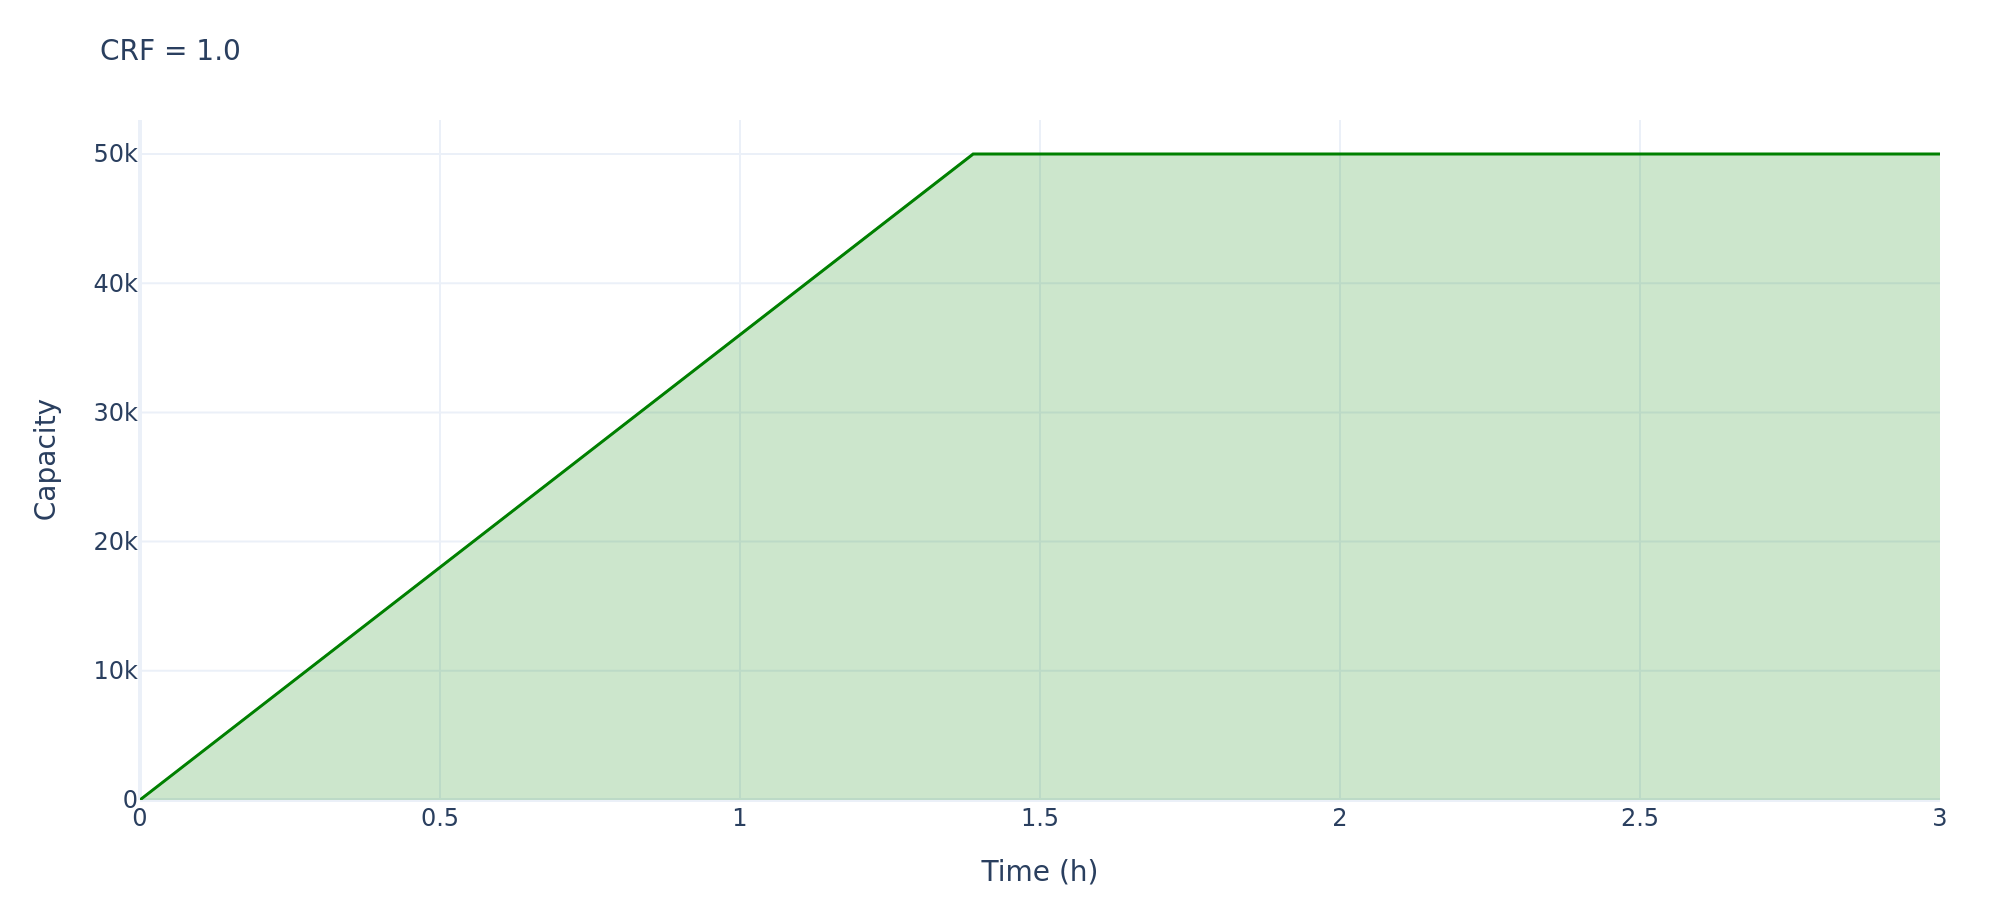
\includegraphics[width=0.42\textwidth]{fig/capacidad_resend_pro_k1.png}}
\subfigure[Resend Pro, $k = 50$ (5 minutos)]{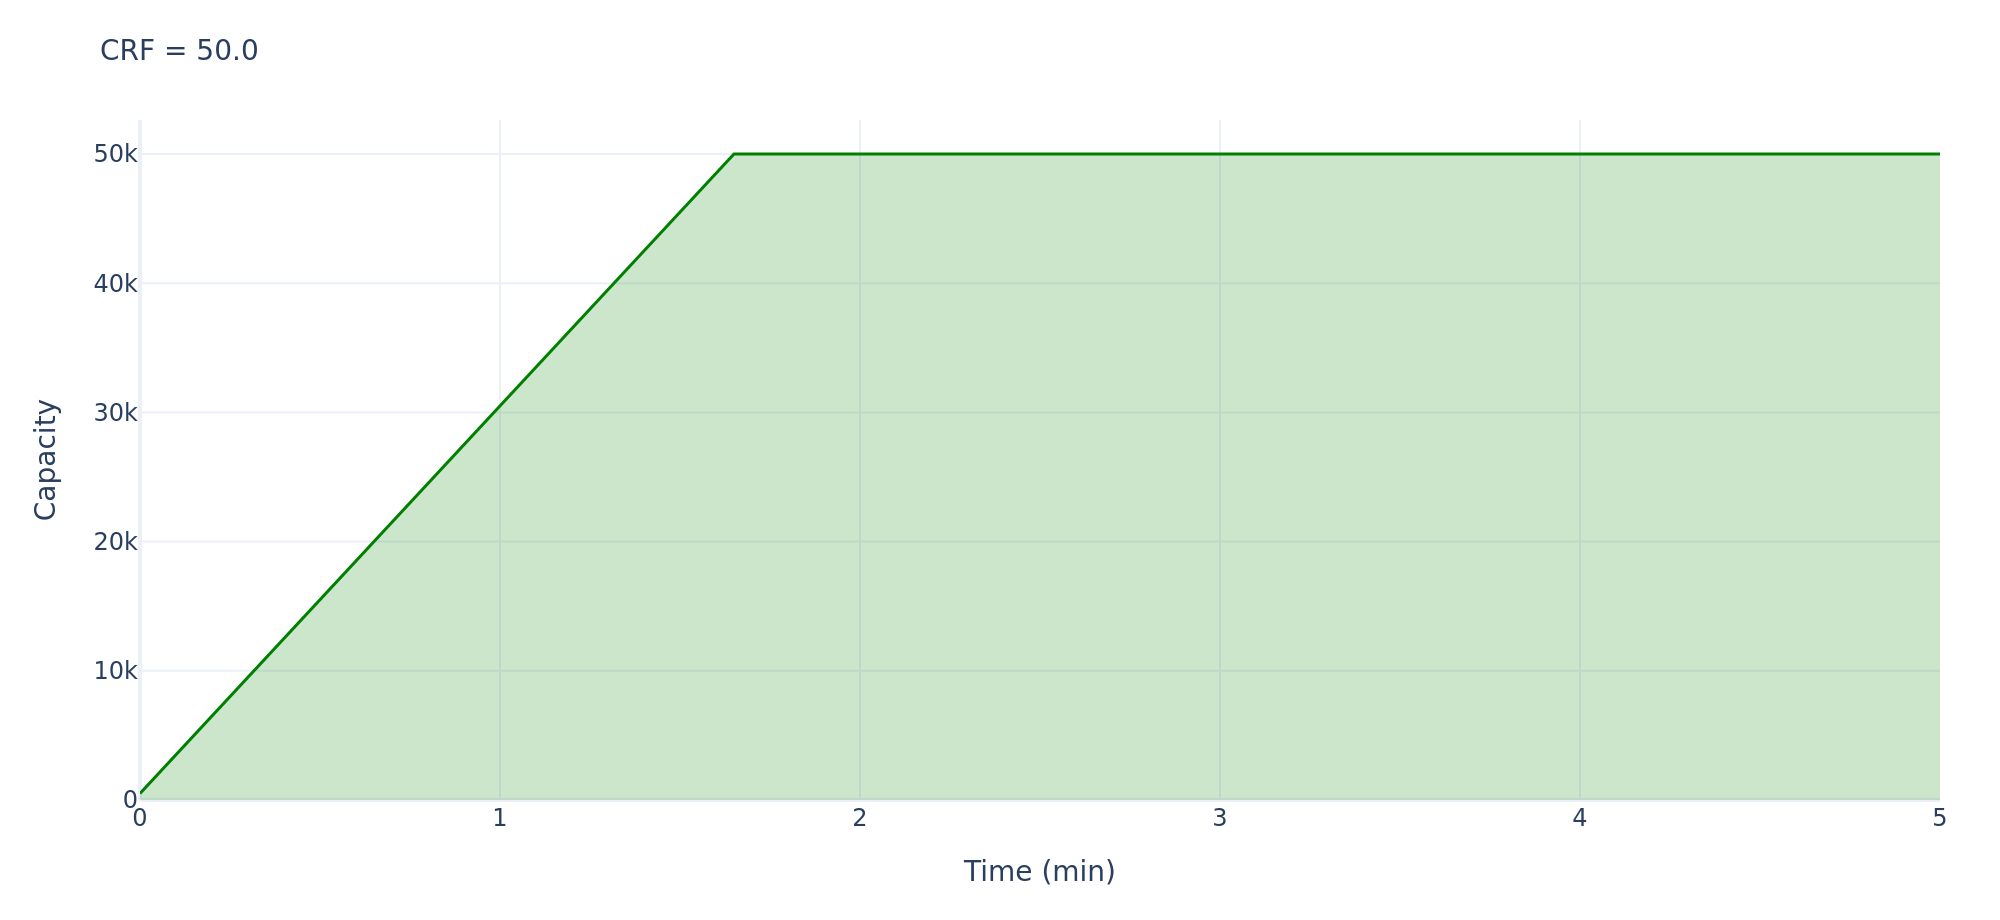
\includegraphics[width=0.42\textwidth]{fig/capacidad_resend_pro_k50.png}}
\subfigure[SendGrid Essentials 50K, $k = 1$ (15 segundos)]{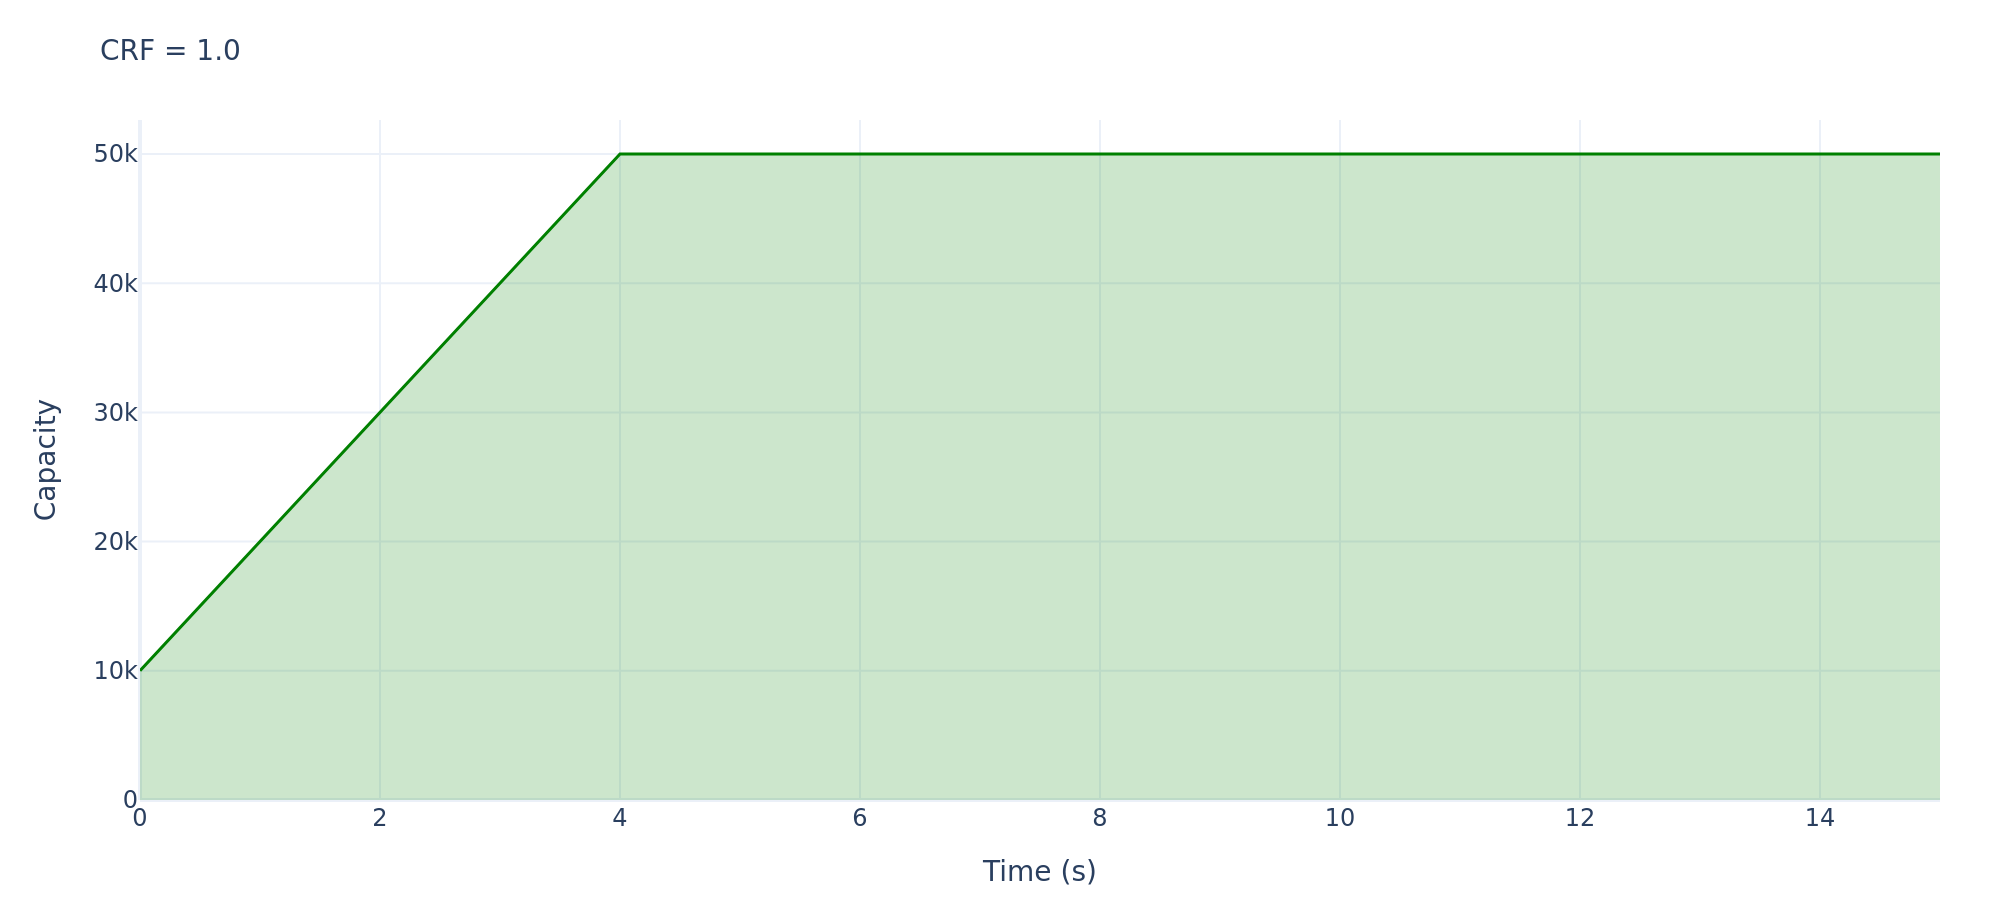
\includegraphics[width=0.42\textwidth]{fig/capacidad_sendgrid_essentials_k1.png}}
\subfigure[SendGrid Essentials 50K, $k = 1.000$ (5 segundos)]{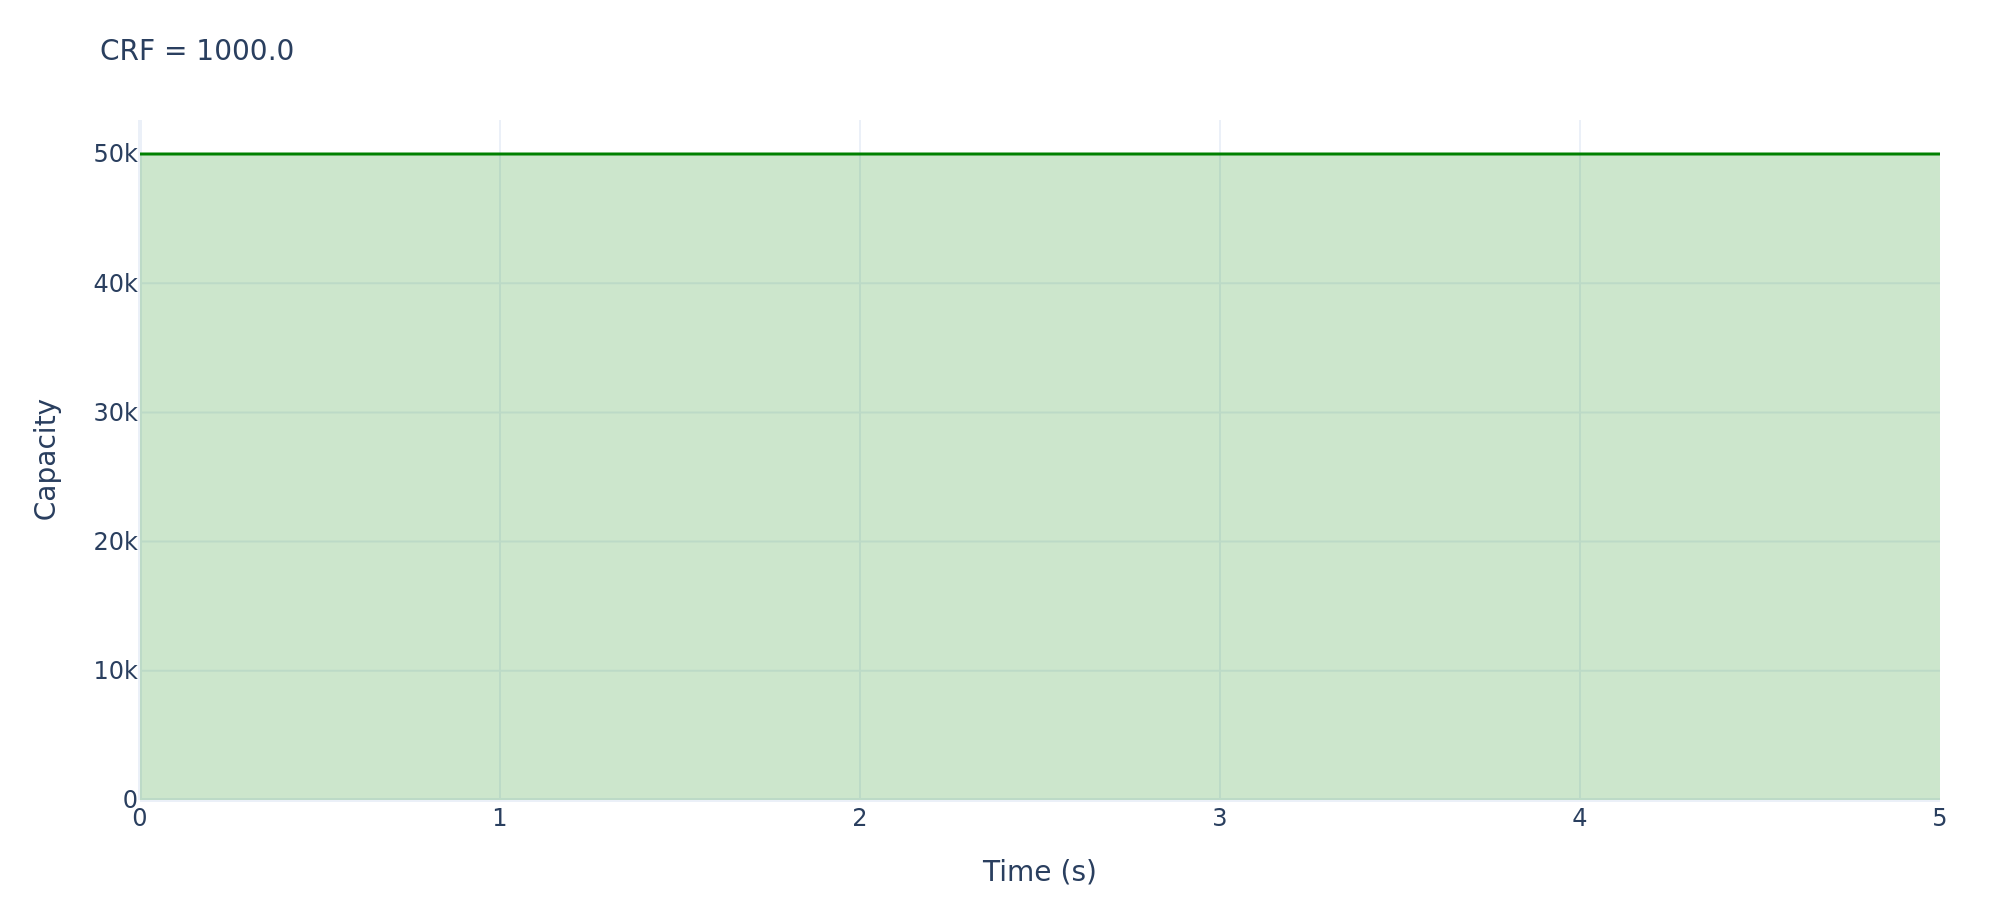
\includegraphics[width=0.42\textwidth]{fig/capacidad_sendgrid_essentials_k1000.png}}
\subfigure[MailerSend Hobby, $k = 1$ (1 hora)]{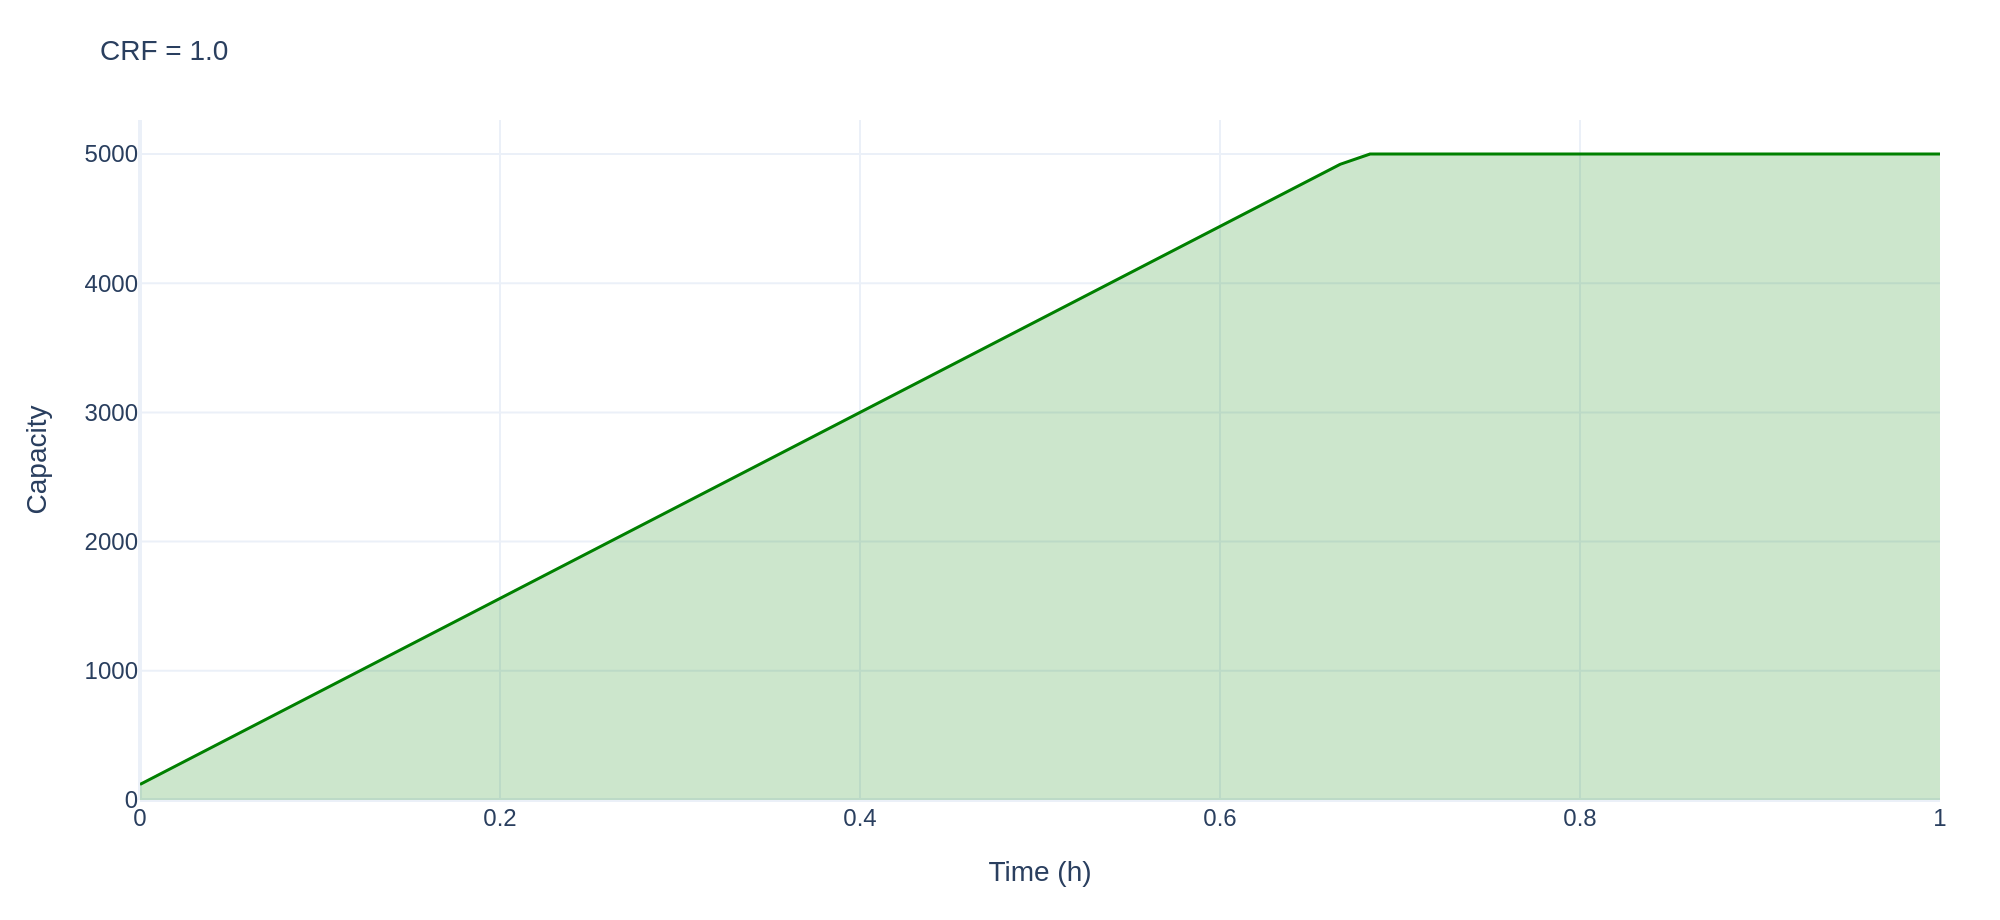
\includegraphics[width=0.42\textwidth]{fig/capacidad_mailersend_hobby_k1.png}}
\subfigure[MailerSend Hobby, $k = 70$ (1 minuto)]{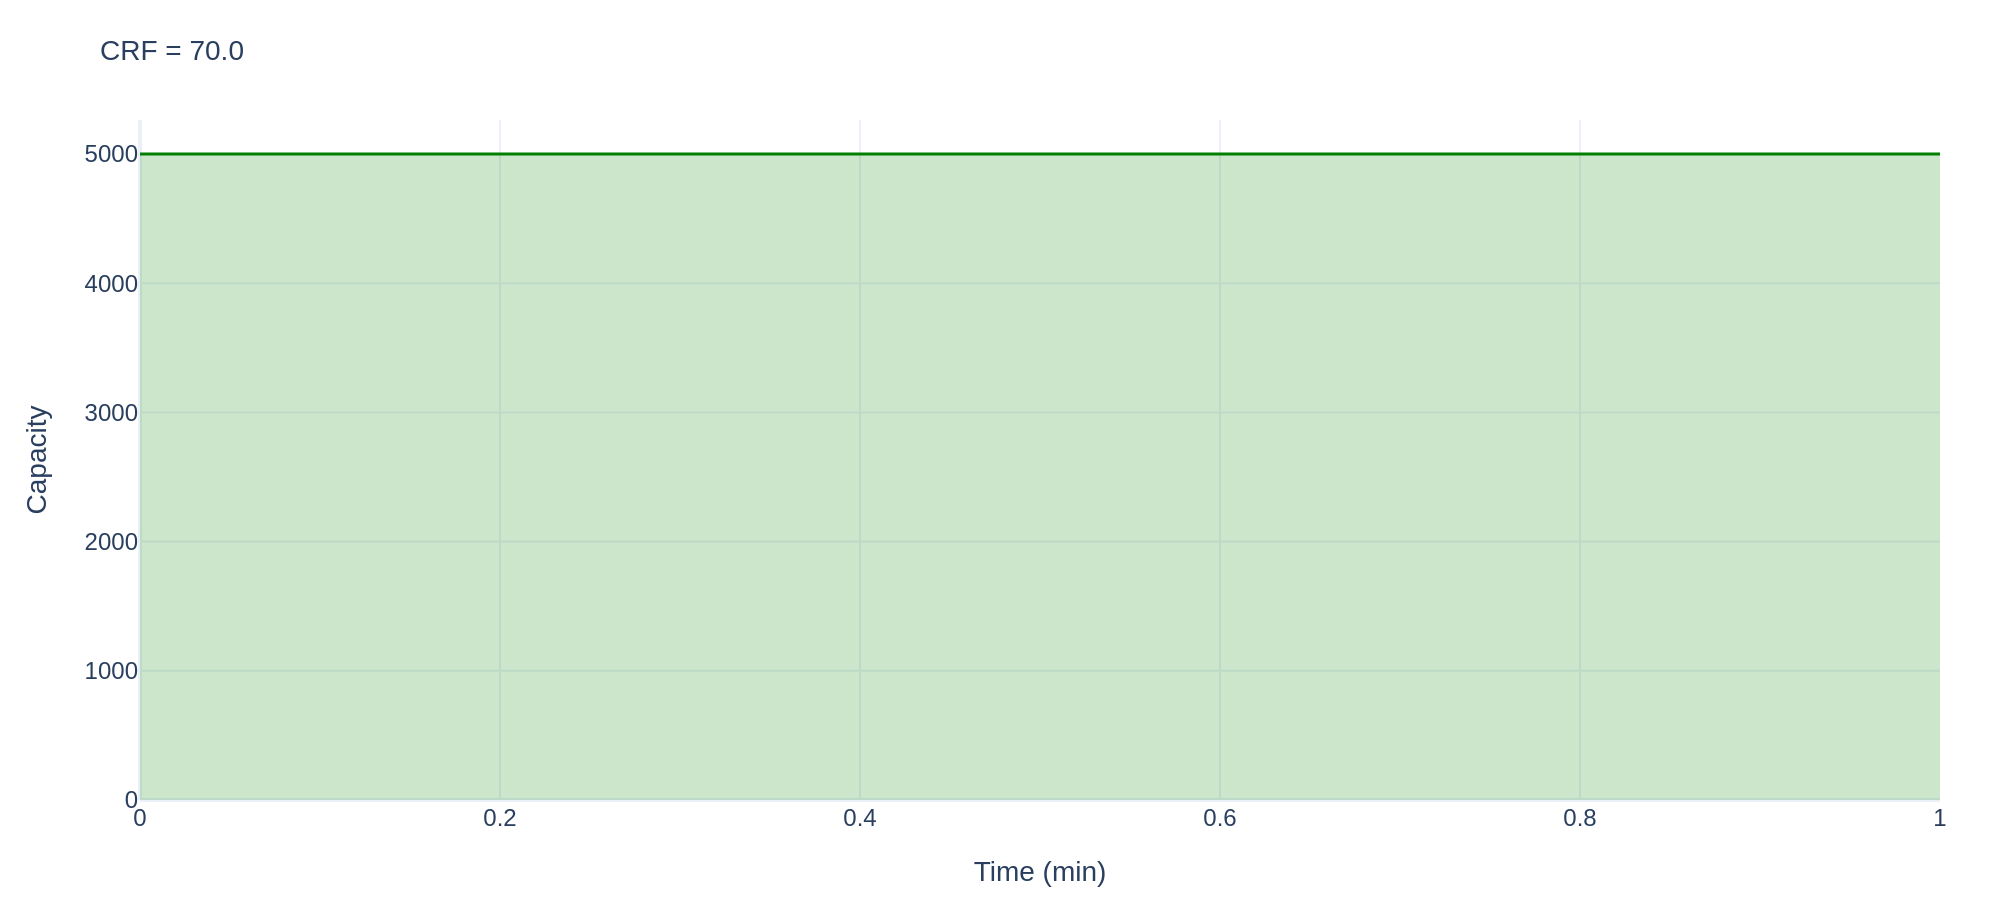
\includegraphics[width=0.42\textwidth]{fig/capacidad_mailersend_hobby_k70.png}}
\subfigure[Amazon SES, los cuatro planes, $k = 1$ (10 minutos)]{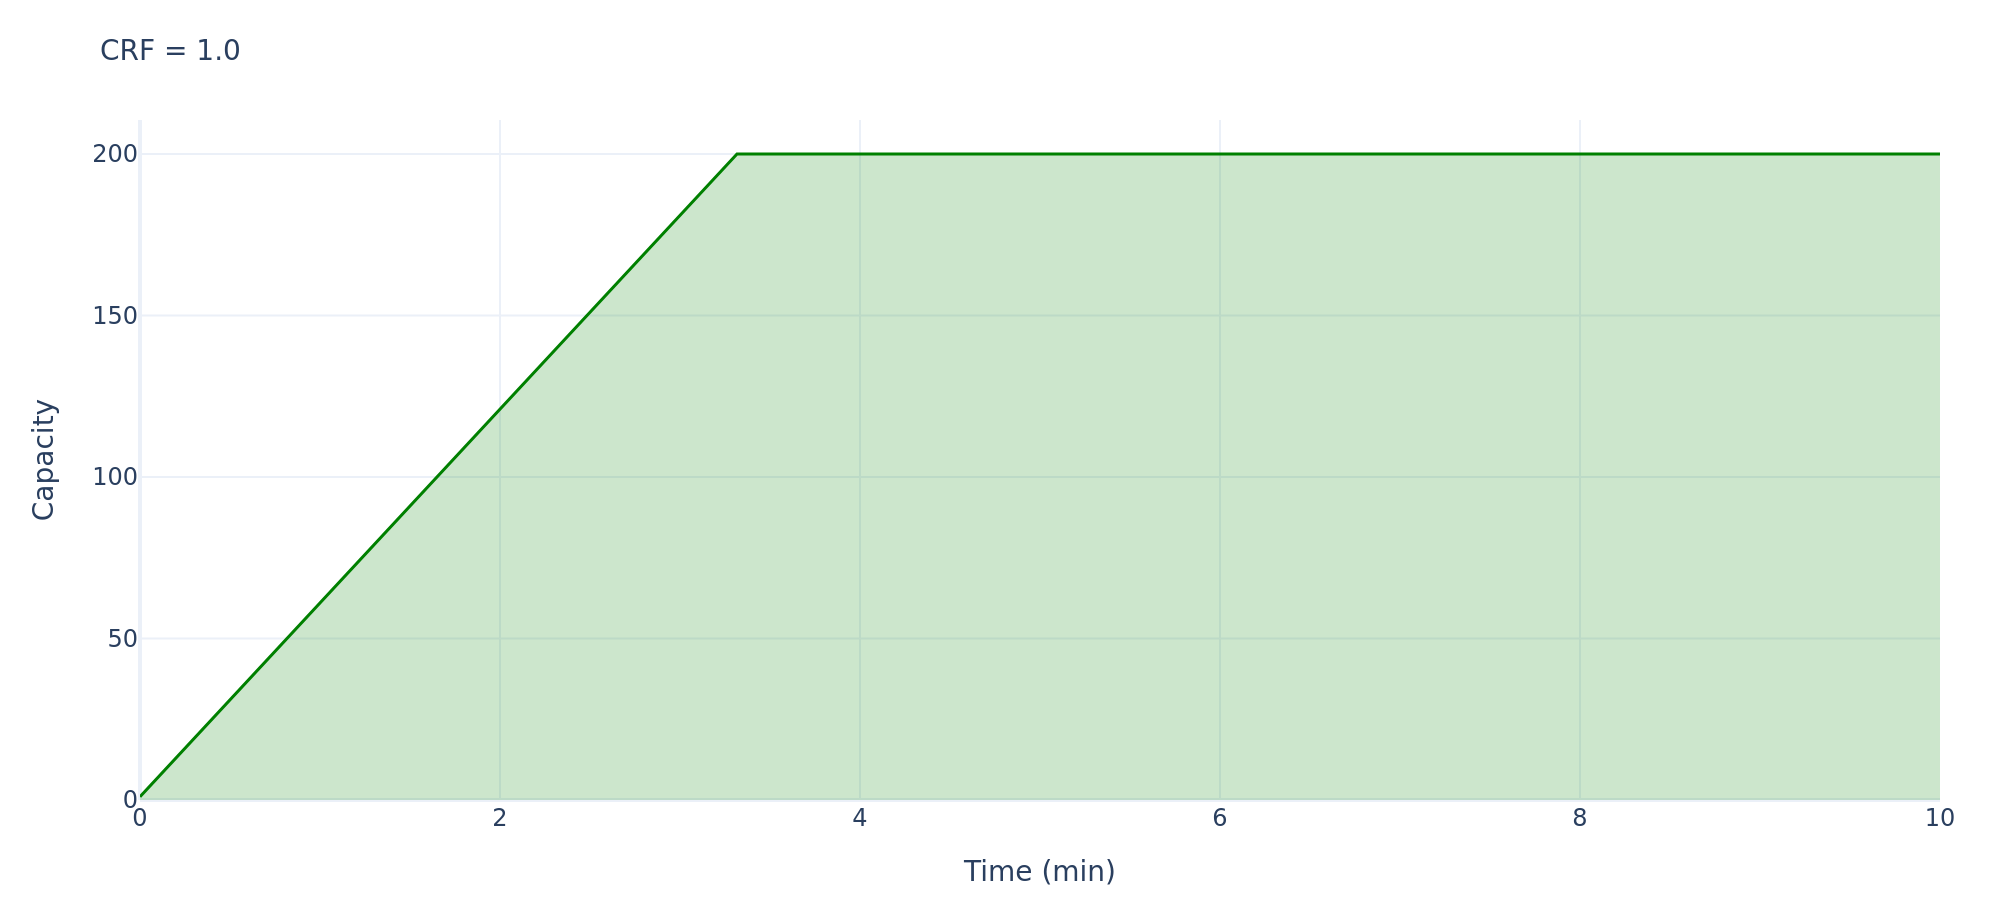
\includegraphics[width=0.42\textwidth]{fig/capacidad_ses_pro_k1.png}}
\subfigure[Amazon SES, los cuatro planes, $k = 50$ (15 segundos)]{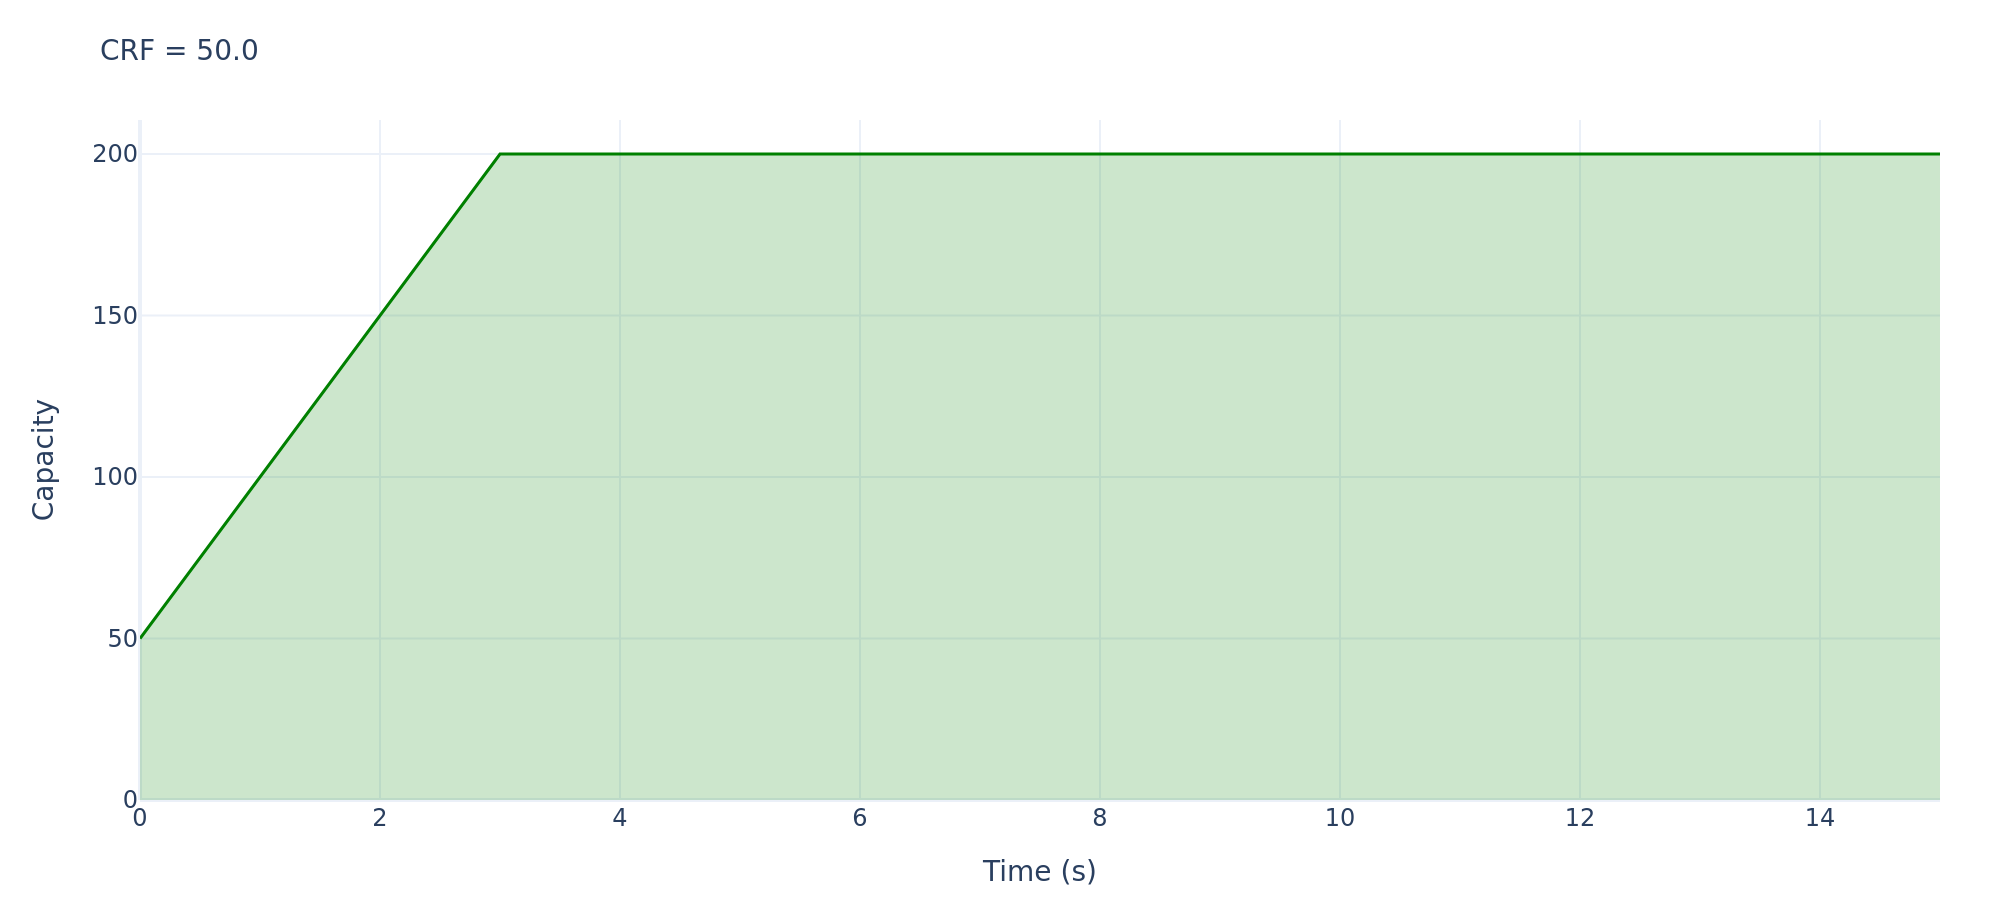
\includegraphics[width=0.42\textwidth]{fig/capacidad_ses_pro_k50.png}}
\caption[Curva de capacidad $C(t)$ de Resend Pro, SendGrid Essentials 50K, MailerSend Hobby y Amazon SES]{Curva de capacidad $C(t)$ de Resend Pro, SendGrid Essentials 50K, MailerSend Hobby y Amazon SES con $k = 1$ y con el $k$ máximo de cada API, dibujada por PRIME4API \citep{prime4apirepo} en local (endpoint \texttt{/datasheet/capacity-curves/chart/inflection}, septiembre de 2026). Cada panel muestra el intervalo que hace visible el codo. A partir de él la curva sigue horizontal hasta que la cuota se repone: al final de la ventana de 30 días en Resend, SendGrid y MailerSend, y cada día en Amazon SES. El área sombreada es la capacidad acumulable. Los ocho paneles son la dimensión de correos, y por eso el panel (e) no incluye la cuota diaria de 1.000 peticiones de Hobby, que el motor evalúa aparte (hallazgo H1 y Figura~\ref{fig:escalera-hobby}). Los paneles (g) y (h) dibujan los cuatro planes de SES a la vez, porque los cuatro devuelven la misma curva: la Datasheet les asigna la misma cuota y el mismo caudal, los del entorno de pruebas. Su codo llega a los 199 segundos con $k = 1$ y a los 3 segundos con $k = 50$, y a partir de ahí la cuenta no envía nada más hasta que la cuota se repone.}
\label{fig:capacidad}
\end{figure}

Las Tablas~\ref{tab:limites-rates} y~\ref{tab:limites-rates-b} se leen también con la interpretación geométrica de la capacidad de Ruiz-Cortés y Ruiz-López \citep{ruizcortes2025cajanegra}, que el ACM adopta como semántica oficial (Sección~\ref{sec:estado:acm}).
La curva de capacidad $C(t)$ de Gavira Sánchez \citep{gavira2026tfm} es el máximo de correos acumulables desde el inicio de la ventana hasta $t$ sin violar ningún límite.
Con un \textit{rate} y una cuota tiene dos tramos.
El primero es una recta de pendiente $R \cdot k$, y en él manda el \textit{rate}.
El segundo es horizontal a la altura de $Q$, y en él manda la cuota.
El codo entre ambos está en $t_{\min}$, y la razón entre la ventana y ese codo es $R \cdot W \cdot k / Q$, el cociente de las tablas multiplicado por $k$.
La Figura~\ref{fig:capacidad} muestra la curva de cuatro casos, Resend Pro, SendGrid Essentials 50K, MailerSend Hobby y Amazon SES, con $k = 1$ y con el $k$ máximo de cada API.
La genera el propio PRIME4API \citep{prime4apirepo}: el motor lee las cuatro Datasheets, construye el BoundedRate de cada plan y su renderizador dibuja la curva, ejecutado en local como el servicio que despliega SPHERE (la misma imagen).
En SES la figura separa el precio de la capacidad.
Sus cuatro planes, de 0 a 500 USD al mes, devuelven la misma curva, así que el precio no mueve el codo ni la meseta.
La curva es la del entorno de pruebas, el único estado de la suscripción que el proveedor cifra. En él la cuota de 200 correos se agota en 199 segundos enviando de uno en uno, y en 3 si cada petición lleva sus 50 destinatarios.
La ejecución del motor como biblioteca devuelve las mismas trazas punto a punto.
El motor cuenta la primera ráfaga en $t = 0$, y por eso da 4.999 segundos donde el cálculo a mano da 5.000.
Cada panel muestra el intervalo que hace visible el codo, porque en una ventana de 30 días el tramo inclinado no se distinguiría de una vertical.
La lectura es la de la tabla, pero a la vista.
En Resend Pro el tramo de \textit{rate} dura 83 minutos con $k = 1$ y 99 segundos con $k = 50$.
En SendGrid Essentials dura 4 segundos con $k = 1$ y menos de uno con $k = 1.000$, porque la cuota cabe en 50 peticiones y la curva nace ya en el techo.
En MailerSend Hobby dura 41 minutos con $k = 1$, con una rampa de 120 correos por minuto, y ninguno con $k = 70$, porque la primera ráfaga (8.400) ya supera los 5.000 de la cuota.
El panel de Hobby con $k = 1$ dibuja el par \textit{rate} y cuota mensual, porque los ocho paneles piden la dimensión de correos y la cuota diaria del plan está publicada en peticiones.
Con esa cuota la curva es una escalera, y el mismo motor la dibuja si se le pide en peticiones: la Figura~\ref{fig:escalera-hobby} la recoge junto al hallazgo H1.
En los seis paneles de Resend, SendGrid y MailerSend el tramo horizontal ocupa casi toda la ventana de 30 días, y el área sombreada, la capacidad acumulable, crece solo en el tramo inclinado.
En los dos de Amazon SES la cuota es diaria: la meseta ocupa casi todo el día, y en la ventana de 30 días la curva es una escalera que llega a 6.000 correos.
Lo que el consumidor ve en la gráfica es que la cuota fija un techo, diario en Amazon SES y de ventana en las demás, y el \textit{rate} solo decide cuánto tarda en tocarlo.
La figura recoge tres planes de tres APIs y el entorno de pruebas de Amazon SES, que la Datasheet asigna por igual a sus cuatro planes.
Las dos formas de las APIs nuevas que no caben en una curva de este tipo ya quedan dichas: los dos contadores de Mailgun sobre la misma ventana y la cuota sin ventana de Mailchimp.

De las dos tablas salen diez afirmaciones sobre RQ3.
Cada una se cuenta sobre las ocho APIs, y no sobre planes ni sobre filas de tarifa.
Una API cumple cuando su ficha tiene el dato que la afirmación necesita y ese dato va en la dirección que la afirmación enuncia.
Hay tres estados más.
«No cumple» es que la ficha tiene el dato y apunta en contra, así que es contraejemplo y se nombra.
«No comprobable» es que la afirmación tiene sentido en esa API pero el dato no existe en ningún hecho, y entonces nunca cuenta a favor.
«No aplica» es que la afirmación presupone una estructura que esa API no tiene, como los planes en Mailchimp o la cuota incluida en SES, y ahí el hueco es del enunciado.
Los denominadores se escriben a favor, en contra, no comprobable y no aplica sobre ocho.
Un margen se calcula con $k = 1$, que solo lo multiplica, así que el margen a $k = 1$ es cota inferior.
Las cuatro primeras afirmaciones venían de la versión de cuatro APIs, y tres de las cuatro se debilitan al pasar a ocho.

La primera: donde hay \textit{rate} y cuota con valor y la cuenta está en estado sano, la cuota es la restricción activa, por entre 2,6 veces y ocho órdenes de magnitud.
Seis a favor, ninguna en contra, una no comprobable y una que no aplica.
Los cocientes van de 2,59 en MailerSend Professional 2M a 129.600.000 en el Free de Postmark, y ese rango no se mueve al pasar de cuatro APIs a ocho.
Lo que se estrecha es el enunciado: «en ningún plan publicado» valía cuando las cuatro APIs del catálogo tenían las dos cifras en su Datasheet.
Con ocho hay que decir en las seis APIs cuya Datasheet lleva \textit{rate} y cuota con valor, publicado o medido.
La no comprobable es SES: fuera del entorno de pruebas el proveedor no publica ninguno de los dos números.
La que no aplica es Mailchimp, y ahí el signo se invierte.
La franquicia son 500 correos sin ventana y el tope horario son 25 correos.
Agotarla lleva veinte horas, y lo único que pone tiempo es el caudal.
Cinco de los seis márgenes descansan en un \textit{rate} que no está publicado como tal, y el único calculado con documentación, panel y cabecera de acuerdo es el de Resend.
Para dimensionar volumen el consumidor puede seguir ignorando el \textit{rate} en seis de las ocho APIs, siempre que la cuenta esté sana.
En SES la pregunta no se puede contestar antes de abrir la cuenta, porque los dos números llegan con el acceso de producción.

La segunda: el \textit{rate} de envío no es una variable del plan y la cuota sí.
Las dos mitades se cuentan aparte, y las dos se debilitan.
La primera va seis a favor, una en contra y una que no aplica.
La segunda va seis a favor y dos que no aplican.
Sostienen la primera mitad seis APIs: Postmark no publica ningún \textit{rate}, Resend publica un valor por equipo, SendGrid un 10.000 sin condición de plan y MailerSend un 120 por minuto para los cuatro planes.
Mailgun no atribuye caudal a ningún plan, y el valor del fichero, medido desde una cuenta Free, se referencia desde los cuatro.
Mailchimp no tiene plan del que el caudal pueda depender, porque lo fija la reputación.
El contraejemplo es Brevo, y la versión de cuatro APIs no lo tenía.
Publica tres categorías de caudal para el mismo endpoint de envío, y una viñeta invita a subir a Enterprise para obtener más.
Subir de plan multiplica por seis el caudal del envío individual, y es la primera vez que eso pasa en el catálogo.
El contraejemplo no está cerrado, y eso también se cuenta: la misma página restringe Advanced a dos planes en una viñeta y lo ofrece a los cinco en el distintivo de su tabla.
La primera mitad no aplica a SES, donde el único caudal publicado es el del entorno de pruebas, un estado de la suscripción, y se aplica por región.
PRIME4API lo confirma leyendo el documento: encuentra cuatro planes y ninguno cambia la capacidad.
La segunda mitad no aplica a dos APIs, y esto es nuevo.
En SES el plan no compra volumen: no hay cuota incluida que comprar, y los cuatro planes devuelven la misma cuota de 200 correos.
Lo que el plan compra son funciones y tramos de precio unitario.
En Mailchimp no hay planes: lo que se compra es la propia unidad de volumen, el bloque de 25.000 correos, a precio degresivo de 20 a 10 USD \citep{mailchimppricing}.
La frase «se compra volumen, no velocidad» deja de valer como regla del dominio.
En Brevo se compran las dos cosas, en SES no se compra ninguna y en Mailchimp lo único que hay que comprar es volumen, sin plan alrededor.
PI-D04 pregunta si sube el \textit{rate} al subir de plan.
Tenía cuatro noes y ahora tiene seis noes y un sí en ámbar.

La tercera: el \textit{rate} publicado y el observado no coinciden, y la señal para el consumidor es la cabecera de respuesta.
La primera mitad va cuatro a favor, tres en contra y una no comprobable, y se cae como afirmación universal.
Sostienen el desajuste cuatro APIs, y la primera es Postmark, que no publica \textit{rate} y devuelve 5.000 en la cabecera de cada respuesta.
SendGrid publica 10.000 para un endpoint que no devuelve cabeceras.
En los endpoints de lectura devuelve 600 y 6, valores que ninguna página documenta.
MailerSend publica 120 por minuto y el sondeo midió 10, porque la cuenta no está aprobada.
Mailgun documenta las tres cabeceras sin publicar ningún umbral, y lo medido es 80.000 peticiones por diez segundos.
Los tres contraejemplos son Resend, que ya coincidía en documentación, panel y cabecera, y dos nuevos.
La cabecera del envío de Brevo devolvió exactamente el 1.000 de su tabla General.
Las tres superficies documentales de Mailchimp y su medición dan el mismo 25 por hora.
Con cuatro APIs el desajuste parecía el estado natural del dominio, y con ocho el enunciado es más estrecho.
Las tres que coinciden publican el valor con su ámbito escrito. Resend lo da por equipo, Brevo ruta a ruta y Mailchimp para la cuenta de prueba. En las cuatro que divergen no está publicado, está en una FAQ o es el de otro estado de la suscripción.
La segunda mitad va cinco a favor, dos en contra y una con reserva, y cambia de sujeto.
SES no emite ninguna cabecera de caudal: la búsqueda sobre su contrato máquina da cero apariciones, y sus nueve respuestas 429 tampoco traen \texttt{retry-after}.
Mailchimp no tiene ninguna cabecera de caudal en ninguna página oficial ni en las respuestas del sondeo, y su tabla oficial de errores no incluye ni 429 ni 403.
La reserva es Mailgun, que emite la cabecera y no deja leerla gratis: solo aparece en un POST aceptado, así que observar el caudal cuesta un envío.
La señal fiable ya no es la cabecera, porque dos de ocho no la tienen y una la cobra, y lo que ocho APIs dejan ver va en la sexta afirmación.
La documentación miente además sobre su propia señal en dos sitios.
Brevo afirma que las cabeceras llegan en todas las respuestas, y llegaron en un 400 y no en dos 200.
El ejemplo de 429 de MailerSend lleva 60 en la cabecera y 120 en el mensaje.
El tercer peldaño de la escalera de validación (Sección~\ref{sec:propuesta:validacion}) es el que ha producido los \textit{rates} observados, y ha llegado a las ocho APIs por dos vías.
En seis el número salió de una cabecera de respuesta: Postmark, Resend, SendGrid, MailerSend, Brevo y Mailgun.
En las dos que no emiten ninguna cabecera de caudal salió de un endpoint de introspección: el de SES y el de Mailchimp.
Y el número observado no siempre responde a la pregunta del plan.
En SendGrid son los \textit{rates} de los endpoints de lectura y no el del envío.
En Postmark y en Mailgun son valores que ninguna página publica.
Y en MailerSend, SES y Mailchimp es el de un estado de la suscripción que la Datasheet modela como alias.

La cuarta: el tope de destinatarios por petición, el CRF, es el factor que conecta el \textit{rate}, en peticiones, con la cuota, en correos.
La primera mitad va siete a favor y una en contra.
La segunda va cinco a favor, dos en contra y una que no aplica.
El tope vale 50 en Postmark, 50 en Resend, 1.000 en SendGrid, 70 en MailerSend, 2.000 en Brevo, 50 en SES y 1.000 por lote en Mailgun.
El contraejemplo es Mailchimp, y el proveedor lo escribe en la misma frase: no hay limitación de destinatarios, pero el JSON de la llamada tiene que pesar menos de 10 MB.
La cota de una llamada está en megabytes y no en destinatarios, así que no hay $k$ que conecte las dos unidades.
La segunda mitad decía que la documentación publica el tope peor de lo que la API lo aplica, y era cuatro de cuatro. Ahora es cinco de ocho.
Los dos contraejemplos son casos en que la documentación acierta.
SES publica el tope como suma y con la definición explícita, «50 recipients per message», y aclara que un destinatario es cualquier dirección de \texttt{To}, \texttt{Cc} o \texttt{Bcc} \citep{sesdocs}.
Resuelve por escrito la ambigüedad que en Postmark, Resend y MailerSend hubo que medir, y ninguna página de SES publica el tope de otra forma.
SendGrid cuenta a favor de la afirmación, aunque su referencia también la resuelve, porque su especificación OpenAPI da el tope por campo y sin total.
El segundo contraejemplo es Mailgun, que publica 1.000 en dos páginas distintas, y la medición devuelve exactamente eso: el destinatario 1.001 da un 400 con el mensaje «Too many recipients, max is 1000».
Lo que queda no es una ley del dominio sino un reparto. Los proveedores que publican el tope por campo lo aplican a la suma, y los que lo publican como suma lo cumplen.
Solo cinco de los siete topes están verificados por sondeo: los de Postmark, Resend y SendGrid, el de Mailgun y el contorno del estado no aprobado de MailerSend.
En Brevo no hay sondeo de destinatarios, y en SES el 50 no se midió y tampoco aparece en la referencia de la operación, solo en la página de cuotas.
Para el consumidor: en SES una petición de 50 destinatarios consume 50 de los 200 diarios del entorno de pruebas, y en Brevo una de 2.000 agota casi siete veces la cuota diaria del plan Free.

Las seis afirmaciones que siguen solo son visibles con ocho APIs.

La quinta: el caudal por cuenta con cifra atribuible a un plan no se publica en siete de las ocho APIs.
La única excepción está en ámbar y con la discrepancia abierta.
La carencia es el caso general, y ninguna de las siete la declara igual en su fichero.
SES la declara como hueco de bloque entero y Mailgun como valor único referenciado desde los cuatro planes.
MailerSend la declara como valor por defecto, y Mailchimp como alias de estado repetido en tres endpoints: el tope es de la cuenta y no del endpoint.
La excepción es Brevo, con las tres categorías ya descritas.
La formulación absoluta, que ningún proveedor publica el caudal por cuenta con cifra atribuible a un plan, no se sostiene: hay uno.
Lo que sí se sostiene es el recuento de siete a uno, y que el único que lo publica no ha conseguido publicarlo sin contradecirse en la misma página.

La sexta: la señal fiable del caudal vigente no es la cabecera sino el endpoint de introspección, y solo lo tienen cuatro de las ocho.
Tres devuelven el límite en vigor.
SES publica los dos topes de la cuenta en un \texttt{GET} que no gasta cuota, y su propia documentación señala ese endpoint como la vía de conocerlos, precisamente porque no devuelve ninguna cabecera.
Mailchimp devuelve la cuota horaria junto a la reputación y el tamaño de la cola en \texttt{POST /users/info}, y MailerSend ofrece \texttt{GET /v1/api-quota}, que tampoco consume cuota.
El cuarto devuelve menos.
El \texttt{GET /v3/account} de Brevo da el saldo de correos y el periodo exacto del ciclo, treinta días anclados al alta, pero ninguno de sus campos es de límite ni de consumo, y la medición corrige a la documentación.
Los cuatro que no lo tienen son Postmark, Resend, SendGrid y Mailgun.
En Mailgun el efecto es el más duro: la cabecera existe y solo llega en un POST aceptado.
La relación entre límite y caudal que el consumidor puede verificar antes de enviar existe en la mitad del catálogo.
En la otra mitad conoce su capacidad real después de gastarla, o no la conoce.
El tercer peldaño del método hereda esa asimetría. Donde hay endpoint de introspección el sondeo cuesta cero envíos, y donde no lo hay medir el caudal exige forzar el rechazo o gastar un envío.

La séptima: la ventana no se declara, y ninguna de las ocho APIs la tiene en verde en todas sus cuotas.
Cada API se clasifica por el peor color que lleva alguna de sus cuotas.
Hay cuatro en rojo (\semrojo{}), cuatro en ámbar (\semambar{}) y ninguna en verde. SendGrid es la que más se acerca: publica la medianoche UTC y el periodo de facturación, y solo la ventana de Premier va en ámbar.
Los cuatro rojos los aportan las APIs nuevas, y responden a tres modos de fallo.
Las dos cuotas del Free de Mailgun y la diaria del Free de Brevo tienen valor y periodo, y ninguna fuente fecha su reposición.
La de SES está en contradicción del propio proveedor, deslizante en una página y fija en otra, y el campo se deja vacío a propósito.
Y la franquicia de Mailchimp no tiene ventana ninguna, porque el proveedor escribe que no caduca ni se renueva, mientras v0.3 exige periodo en toda cuota.
La ventana del caudal no la declara ninguna de las ocho.
Dos sondeos la acotaron sin fijar su tipo. En Brevo la ruta de actividad volvió a admitir peticiones antes de cumplirse un segundo desde la primera de la serie. En Mailgun dura unos diez segundos y la abre el uso, pero las cabeceras no separan una ventana fija de una deslizante.
Ninguna de las dos medidas decide qué tipo de ventana de v0.3 le corresponde.
Saber cuántos correos entran no basta para saber cuándo entran.
En cuatro APIs el ancla del contador no existe en ninguna fuente, así que el consumidor no puede calcular cuándo su cuota vuelve a cero sin observarlo en su propia cuenta.

La octava: el estado de la suscripción y la reputación explican más de la capacidad observada que el plan.
Seis de las ocho publican al menos un estado que condiciona la capacidad, tres de esas seis publican una cifra distinta por estado, y en tres la capacidad medida es la del estado y no la del plan.
MailerSend baja de 120 a 10 peticiones por minuto con la cuenta bajo revisión, y el lote de 10 a 1.
SES publica los dos topes del entorno de pruebas y no los de producción.
Documenta además tres valores de \texttt{EnforcementStatus}: «Healthy», «Probation» y «Shutdown».
Mailchimp fija 25 correos por hora en la cuenta de prueba y ata la de pago a la reputación, que su propio panel codifica en cuatro niveles.
Los otros tres estados no llevan cifra.
Resend amplía el caudal a los remitentes de confianza bajo petición, sin publicar cuánto.
Mailgun describe el arranque de una cuenta nueva sin una sola cifra, y Postmark condiciona el cambio de plan a la aprobación de la cuenta.
Con cuatro APIs esto era un rasgo de MailerSend, y con ocho el plan ya no basta para leer la capacidad observada.
El esquema lo nota.
SES modela el estado como alias con el vocabulario del proveedor, \texttt{sandbox}, colgado de las dos rutas de envío en los cuatro planes, y Mailchimp repite el alias \texttt{demo} en sus tres endpoints de envío por el mismo motivo.
Lo que ninguna de las seis publica es el umbral que dispara el cambio de estado.

La novena: el sobrecoste deja de ser universal, porque cinco de las ocho lo tienen y tres no, y cada una de esas tres pone algo distinto en su lugar.
En las cinco que lo tienen el precio del exceso baja con el volumen.
Postmark va de 1,80 a 1,70 USD por mil, Resend de 0,90 a 0,46 y MailerSend de 1,50 a 0,50.
SendGrid lo cobra por correo, de 0,0013 a 0,0005, y Mailgun va de 1,80 a 0,40 \citep{mailgunpricing}.
Brevo no publica ninguna cifra de exceso en ninguna de las cuatro páginas buscadas, y lo más cercano es la negación de que haya cargos adicionales \citep{brevopricing}.
Su lugar lo ocupa un ascenso automático de plan disparado por el número de contactos, que no es una cuota de correo.
SES no tiene sobrecoste porque no tiene cuota incluida, y sus tramos de precio bajan al subir de volumen sin corte ni penalización \citep{sespricing}.
Mailchimp convierte el agotamiento en un muro, y lo que ocupa el lugar del sobrecoste es comprar otro bloque del mismo producto.
El borde de la cuota tiene ya tres comportamientos documentados.
SES descarta el mensaje y no lo reintenta, mientras SendGrid, MailerSend y Mailchimp levantan un muro. Brevo retiene hasta 1.000 correos y descarta en silencio lo que pasa de ahí.
El caso que junta las dos formas es Mailchimp: su cuota es muro y su caudal es cola, en la misma cuenta, y el atraso se reprocesa en la hora siguiente.
El coste de pasarse de la cuota solo es comparable entre cinco APIs, y en las otras tres la pregunta cambia de forma.

La décima: la unidad de la cuota se confirma midiendo o no se confirma. Cuatro de ocho tienen respaldo, y dos de esos cuatro salieron del tercer peldaño.
Con respaldo documental hay dos, Resend y SendGrid, que escriben que cada destinatario consume una unidad.
Con respaldo medido hay dos, y los dos son de la tanda de las cuatro APIs nuevas.
En Brevo el saldo de la cuenta bajó de 300 a 298 tras una petición con dos destinatarios, y se mantuvo estable noventa segundos después.
En SES el contador marcó 5,0 sobre 200 tras cuatro mensajes aceptados con cinco destinatarios, uno de ellos con la misma dirección en \texttt{to} y en \texttt{cc}.
Ese cinco descarta a la vez el mensaje como unidad y la deduplicación de direcciones, que habrían dado cuatro las dos.
Sin respaldo quedan cuatro: Postmark no confirma el cómputo por destinatario, MailerSend lo tiene modelado y no publicado, en Mailgun es inferencia declarada y en Mailchimp el artículo del proveedor que lo trataría devolvió un 403.
Si la unidad de la cuota no está confirmada, el factor $k$ de la cuarta afirmación no conecta nada.
Multiplica peticiones por destinatarios para obtener correos, y en cuatro APIs no consta que un destinatario sea un correo a efectos de contador.
La cadena entera de RQ3 descansa en un dato que la mitad del catálogo no publica y que solo se cierra midiendo.

Lo que deja de valer al pasar de cuatro APIs a ocho no es una cifra, sino la lectura de que el catálogo describe un dominio homogéneo.
Con cuatro APIs las cuatro tenían planes, cuota mensual, sobrecoste decreciente y tope de destinatarios.
Con ocho, una no tiene planes, una no tiene cuota incluida, tres no tienen sobrecoste y una no tiene tope de destinatarios.
Las cuatro primeras no eran el dominio: eran su parte regular.

Estos cálculos corresponden a operaciones del catálogo Q1--Q10 de PRIME4API, de Gavira Sánchez \citep{gavira2026tfm}, motor de análisis de la capacidad sobre las Datasheets.
La restricción activa a consumo uniforme responde a Q5 (si una demanda con \textit{rate} y cuota puede sostenerse durante un período), la misma operación que resuelve PI-D01 y PI-D02 en la Tabla~\ref{tab:catalogo-pi-2}.
El tiempo mínimo de agotamiento $t_{\min}$ responde a Q2 (o a Q1 con el volumen igual a la cuota), y el factor $k^{*} = Q/(R \cdot W)$ a Q9 (qué CRF hace que ambos límites se agoten a la vez).
Q9 se define sobre dos cuotas, y aquí se aplica al par \textit{rate} y cuota tratando el \textit{rate} como un límite con ventana de un segundo.
Ese factor es el inverso del cociente de las dos tablas, así que se lee en ellas sin calcular nada aparte.
Vale 0,0019 en Resend Pro, $1{,}9 \cdot 10^{-6}$ en SendGrid Essentials, 0,00096 en MailerSend Hobby y 0,0023 en el entorno de pruebas de SES.
Las dos tablas tienen una sola fila con cociente menor que uno, MailerSend Starter 1M bajo revisión, y es la única con $k^{*}$ mayor que uno: 2,31.
Ningún $k \geq 1$ iguala los dos límites en ningún plan publicado con la cuenta sana.
En Mailchimp Q9 no se puede plantear: el caudal ya está en correos y $k$ no multiplica.
El tope de sobrecoste de SendGrid (diez veces el plan, 500.000 correos en Essentials 50K) entra en Q10 (importe del sobrecoste), porque acota el volumen que la cuota admite pagando.

Las mismas operaciones se han ejecutado después contra PRIME4API como servicio REST en local, sobre las ocho Datasheets, con petición y respuesta archivadas por pregunta.
Sobre Postmark, Resend y SendGrid el servicio se arrancó a mano, y sobre las otras cinco es el que despliega SPHERE en local.
El motor reproduce el cálculo a mano en Resend y SendGrid, con tres convenciones propias y una regla de herencia.
Cuenta la primera ráfaga en $t = 0$ (4.999 segundos donde a mano salen 5.000), abre la ventana siguiente en el instante final de un intervalo, y solo conoce el primer volumen contratable de cada plan (F-02).
Q9 no tiene operación directa: el motor devuelve el tiempo de agotamiento de cada cuota para cada CRF, y $k^{*}$ se deriva de esos tiempos.
La regla de herencia suma los límites del plan a los del endpoint: un \textit{rate} declarado en el plan y repetido en el endpoint cuenta dos veces.
En SendGrid Essentials esa repetición aplanaba la curva con $k = 1$ en el primer segundo y duplicaba el techo a 30 días con $k = 1.000$: 100.000 correos donde el proveedor publica 50.000.
El catálogo declara desde entonces cada límite una sola vez, en el plan si vale para todos los endpoints y en el endpoint si es propio, y el validador falla cuando se repite.
La Figura~\ref{fig:capacidad} es la que devuelve el motor sobre la Datasheet, sin variante.
En Postmark el motor mostró primero lo que hace un \texttt{max\_power} vacío.
Con el \textit{rate} sin adoptar respondió 0 segundos para agotar la cuota de Basic y 270 días para 100.000 correos, nueve renovaciones de 10.000, como si el \textit{rate} fuese infinito.
No se equivocaba, hacía lo que el esquema le dejaba hacer, y es la confusión entre «no publicado» y «sin límite» que la propuesta P-04 del Capítulo~\ref{cap:evolucion} quiere impedir.
Con el valor de 5.000 adoptado en ámbar las mismas preguntas se reejecutaron.
El motor responde 1 segundo para agotar la cuota de Basic (2 a mano, por la convención de la primera ráfaga), 270 días y 1 segundo para los 100.000 correos, y devuelve el \textit{rate} donde antes devolvía una lista vacía.
La capacidad a un mes con presupuesto sin tope pasa de $1{,}1 \cdot 10^{12}$ correos, acotada solo por el presupuesto, a 12.960.005.000, que es $R \cdot W$ más la ráfaga inicial.
El veredicto sobre el pico de 20.000 correos en una hora sigue siendo negativo en los cuatro planes, pero la etiqueta cambia de \texttt{rate\_exceeded} a \texttt{quota\_exceeded}.
Con el \textit{rate} vacío el motor atribuía al \textit{rate} una violación de cuota.

Sobre MailerSend las diez preguntas P se ejecutaron el 2026-09-08 contra el mismo servicio, con 15 llamadas archivadas.
Doce coinciden con el cálculo a mano y tres difieren por convenciones ya conocidas.
Sin presupuesto la cuota con sobrecoste es dura, así que 100.000 correos en Hobby tardan 570 días y 41 minutos (19 renovaciones de 5.000), y en $t = 30$ días el motor suma la primera ráfaga de la ventana siguiente.

Sobre las cuatro APIs nuevas las diez preguntas se ejecutaron el 2026-09-21 contra ese mismo servicio.
Son 40 instancias y 68 llamadas archivadas.
Por HTTP responden 16 de 17 en Brevo, 17 de 17 en Mailgun y en SES, y 3 de 17 en Mailchimp.
De las 30 instancias que el motor contesta ninguna difiere del cálculo a mano, y las diferencias que aparecen son las tres convenciones ya descritas.
Las catorce llamadas que Mailchimp no contesta salen de dos huecos deliberados del fichero: el tope del \texttt{workload} de envío y el periodo de la franquicia de 500 correos.
Aislados por sustitución en memoria, rellenar solo el tope cambia el error de \texttt{NoneType} a \texttt{division by zero}, y rellenar además el periodo devuelve 200.
Es la factura medida de un hueco que el esquema obliga a dejar, y va al Capítulo~\ref{cap:evolucion}.
En SES el plan no cambia la respuesta del motor: los cuatro planes devuelven 200 correos al día, una petición por segundo, 1.401 correos en siete días y 6.001 al mes, todo colgado del alias \texttt{sandbox}.
Y SES deja el primer caso del catálogo en que la demanda viola en el instante cero y por el caudal.
PI-B05 pide 20.000 correos en una hora y el motor responde NO en los cuatro planes con la etiqueta \texttt{rate\_exceeded}, porque una petición por segundo no sostiene 5,56 correos por segundo.

La cuota dura sin presupuesto no es un detalle de MailerSend: gobierna la respuesta de PI-A06 en las ocho APIs, y el catálogo la reejecutó con los dos regímenes.
La Tabla~\ref{tab:a06-presupuesto} los pone al lado.
Sin presupuesto el motor cuenta renovaciones de la cuota y el tiempo se mide en meses. Con un presupuesto que no limita expande la cuota con su \textit{overage cost} y el tiempo lo fija el caudal.
Las dos cifras son del proveedor: el sobrecoste lo publica él, y ninguna de las dos es una hipótesis del trabajo.
La segunda no exige elegir presupuesto, porque la respuesta satura en el coste del propio objetivo.
En Hobby, donde 100.000 correos cuestan 149,50 USD, con 149,40 el motor responde 30 días y con 149,50 responde 13 horas y 53 minutos, igual que con mil millones.
La tanda de las cuatro APIs nuevas añade los dos primeros casos negativos del régimen.
En Mailgun Basic el presupuesto alto baja el tiempo de 100.000 correos de 270 días a 1 minuto y 6 segundos.
En Brevo Starter y en SES Pro la misma llamada no mueve un segundo, porque sus cuotas no declaran sobrecoste.
El régimen no es entonces una convención del motor: es una propiedad del \textit{pricing}.
La distancia entre las dos columnas llega a seis órdenes de magnitud, de 270 días a 19 segundos en Postmark Basic con $k = 1$.
Y el esquema no dice cuál de los dos regímenes describe el plan: la cuota lleva su sobrecoste, pero nada declara si el proveedor lo aplica solo, lo exige aprobar o lo tapa un tope.
Es el elemento no soportado F-13 visto desde el motor, y va al Capítulo~\ref{cap:evolucion}.

\begin{table}[H]
\centering
\small
\begin{tabular}{|l|c|r|r|}
\hline
\textbf{API y plan} & \textbf{$k$} & \textbf{Cuota dura} & \textbf{Presupuesto que no limita} \\
\hline
Postmark Basic          & 1     & 270 d 1 s            & 19 s \\
                        & 50    & 270 d                & 0 s \\
\hline
Resend Pro              & 1     & 30 d 1 h 23 min 19 s & 2 h 46 min 39 s \\
                        & 50    & 30 d 1 min 39 s      & 3 min 19 s \\
\hline
SendGrid Essentials 50K & 1     & 30 d 4 s             & 9 s \\
                        & 1.000 & 30 d                 & 0 s \\
\hline
MailerSend Hobby        & 1     & 570 d 41 min         & 13 h 53 min \\
                        & 70    & 570 d                & 11 min \\
\hline
Brevo Starter           & 1     & 570 d 4 s            & 570 d 4 s \\
                        & 2.000 & 570 d                & 570 d \\
\hline
SES Pro (\texttt{sandbox}) & 1  & 499 d 3 min 19 s     & 499 d 3 min 19 s \\
                        & 50    & 499 d 3 s            & 499 d 3 s \\
\hline
Mailgun Basic           & 1     & 270 d 6 s            & 1 min 6 s \\
                        & 1.000 & 270 d                & 0 s \\
\hline
\end{tabular}
\caption[PI-A06 con la cuota dura y con presupuesto que no limita]{Tiempo mínimo para enviar 100.000 correos en un plan de pago de cada API, respondido por PRIME4API \citep{prime4apirepo} en los dos regímenes: sin \texttt{max\_budget}, donde la cuota con sobrecoste se trata como dura y el motor cuenta renovaciones, y con un presupuesto que no limita, donde la expande y manda el caudal. Las respuestas del régimen con presupuesto saturan en el coste del objetivo, así que no dependen del valor que se pase por encima de él. Brevo y SES son los dos casos negativos: sus cuotas no declaran sobrecoste, y por eso las dos columnas coinciden. Las filas de SES son las del alias \texttt{sandbox}, el único estado que el proveedor cifra. Mailchimp no aparece porque sus cuatro llamadas devuelven 500. Las treinta y dos llamadas están archivadas en el repositorio de datos.}
\label{tab:a06-presupuesto}
\end{table}
En MailerSend los veredictos de precio son los del cálculo a mano: Starter a 35 USD para 40.000 correos, y Hobby a 17,5 para 12.000 y a 37 para 25.000.
El de demanda también: NO en los cuatro planes al pico de 20.000 correos en una hora, con la etiqueta \texttt{rate\_exceeded} y la primera violación a los 21,6 segundos.
Dos hallazgos sobre el motor son nuevos, y los dos se han reproducido con el código del motor sobre el mismo YAML.
El primero (H1): la cuota de plan en peticiones se hereda, y \texttt{/quotas} la lista junto a la mensual, pero no entra en la dimensión de correos con la que responden las diez preguntas.
El motor multiplica por $k$ los \textit{rates} en peticiones y no hace lo mismo con las cuotas en peticiones.
Por eso sus cifras de Hobby con $k = 1$ son las del par \textit{rate} y cuota mensual: 41 minutos para agotar los 5.000, 5.184.120 correos al mes con presupuesto sin tope y 33.786,67 con 50 USD.
Con la cuota diaria salen 4 días y 8 minutos, 30.000 y 30.000.
La curva de la Figura~\ref{fig:capacidad} tiene la misma ausencia.
El motor sí calcula esa cuota, pero en otra dimensión: pedida la curva en peticiones devuelve la escalera de la Figura~\ref{fig:escalera-hobby}, con la cuota diaria del plan y la mensual del endpoint convertida por $k$.
De las tres conversiones que el factor $k$ permite, el motor hace dos: el caudal de peticiones a correos y la cuota mensual de correos a peticiones.
La que omite es la cuota diaria en peticiones llevada a correos.
Su renderizador oculta además por defecto la dimensión de peticiones derivada de un \textit{workload}, que hay que pedir con \texttt{show\_derived\_requests}.
En SendGrid no se notó porque su cuota de plan ya está en correos, la dimensión en la que responden las preguntas.
MailerSend es la primera API del catálogo cuya cuota de plan está en otra unidad que la del endpoint.
Ningún veredicto de plan más barato cambia con ello, y el hueco se trata en el Apartado~\ref{subsec:evolucion:h1}.

\begin{figure}[H]
\centering
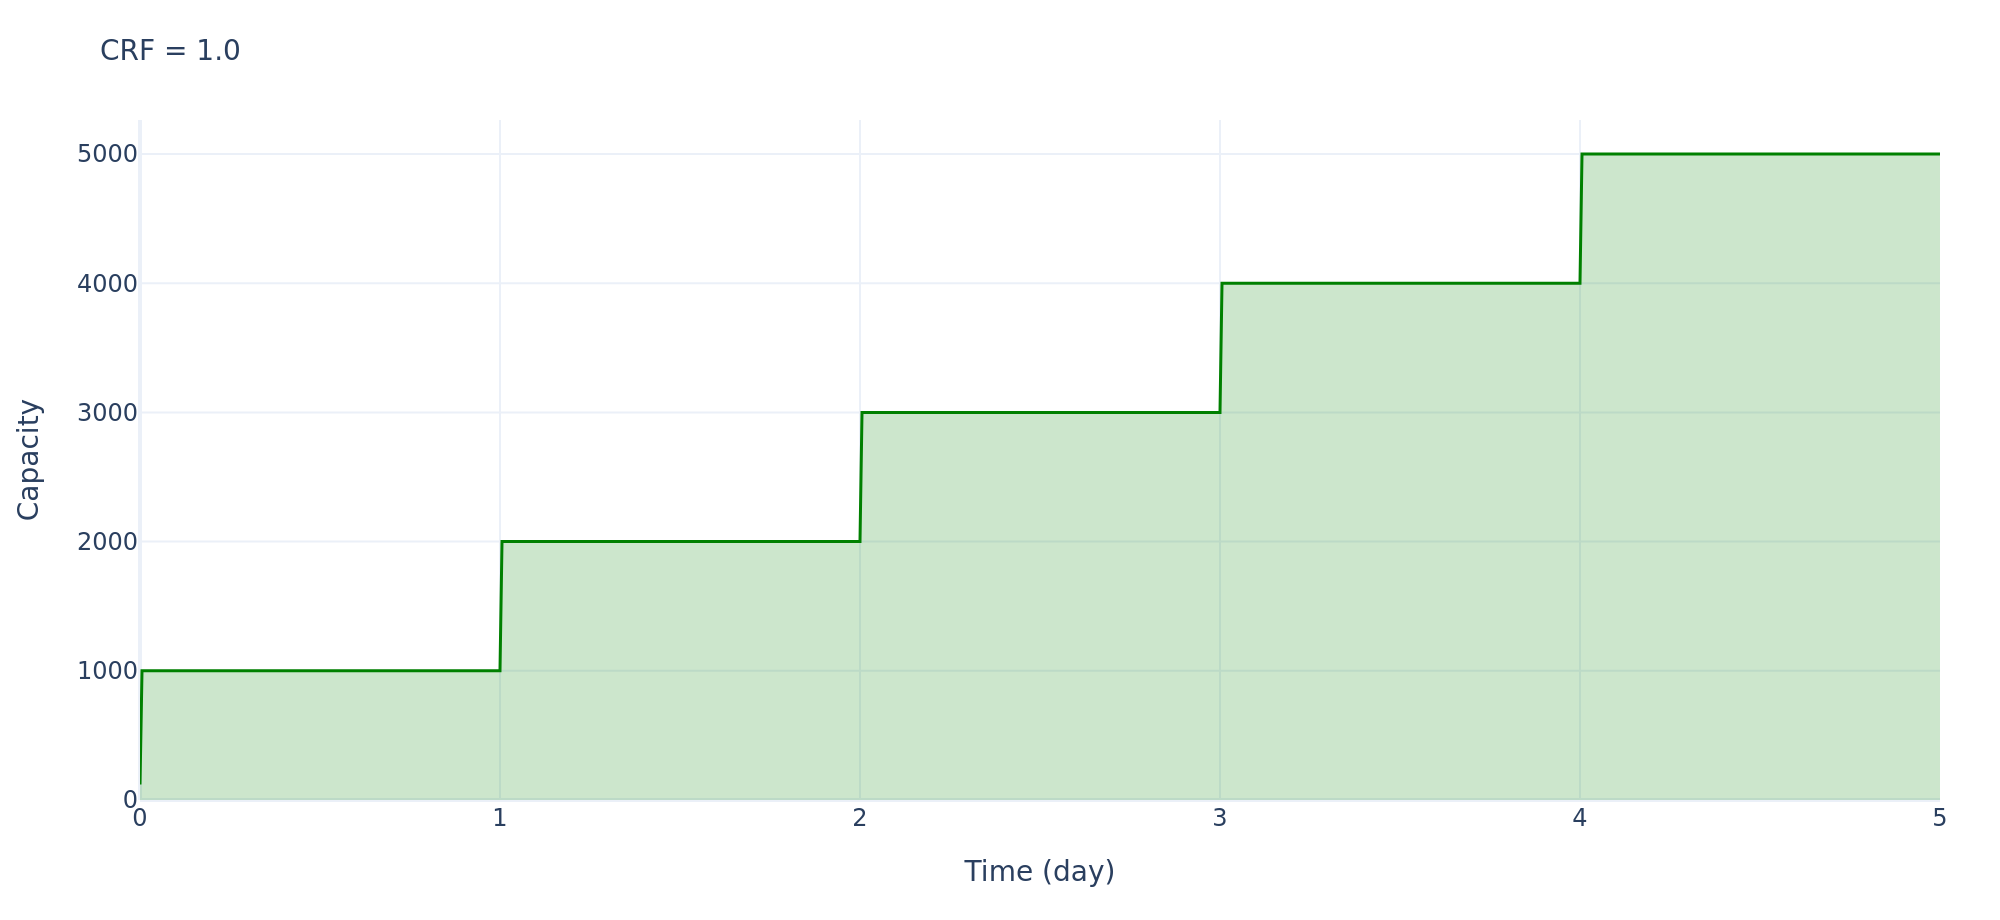
\includegraphics[width=0.72\textwidth]{fig/capacidad_mailersend_hobby_k1_peticiones.png}
\caption[Curva de capacidad de MailerSend Hobby en la dimensión de peticiones]{Curva de capacidad de MailerSend Hobby con $k = 1$ sobre cinco días, pedida a PRIME4API \citep{prime4apirepo} en la dimensión de peticiones: la misma llamada que los paneles de la Figura~\ref{fig:capacidad} con \texttt{capacity\_unit} en peticiones. Aquí sí entra la cuota diaria de 1.000 peticiones del plan, y la curva es una escalera que sube 1.000 cada medianoche UTC hasta los 5.000 de la cuota mensual el quinto día. Con $k = 1$ cada petición lleva un correo, así que la escalera se lee también en correos. El tramo de \textit{rate} (120 por minuto hasta el primer millar, ocho minutos) no se distingue a esta escala.}
\label{fig:escalera-hobby}
\end{figure}
El segundo (H2): \texttt{/capacity-at} con un presupuesto menor que el precio del plan devuelve la cuota base más la ráfaga, 50.120 correos en Professional con 50 USD.
No marca el plan como no asequible, cosa que \texttt{/budget/recommendation} sí hace.
Revisado con ese hallazgo, SendGrid Pro (89,95 USD) había respondido 110.000 con 50 USD de presupuesto en la misma pregunta y no se había anotado.
H2 recurre en la tanda de las cuatro APIs nuevas, y el caso es Brevo Professional, que cuesta 499 USD al mes.
Con 50 de presupuesto el motor devuelve igualmente 151.000 y 152.000 correos: aplica el presupuesto a la expansión de la cuota y no al precio del plan.
Las dos cifras son la misma capacidad con dos categorías de caudal: 150.000 de cuota más 1.000 con el General y más 2.000 con el Advanced.
Los tramos de caudal no cambian el volumen del mes, cambian cuántos correos caben en el primer segundo de la ventana siguiente.
Y la etiqueta \texttt{unreachable\_reason: rate\_limit} con causa de cuota aparece ya en cuatro de las ocho, Postmark, Resend, Brevo y SES.
Los tres son candidatos a incidencia en el repositorio del motor. Antes hay que comprobar si ya existen.

El límite de esta sección es su base. Son ocho APIs.
El par \textit{rate} y cuota con valor en la Datasheet solo se forma en seis.
De esas seis, el \textit{rate} lo publica el proveedor en cuatro, y en dos sale de una cabecera medida, Postmark y Mailgun.
Ninguno de los cuatro publicados es una cifra firme.
El de SendGrid aparece una sola vez en una FAQ sin condición de plan, y el de Resend es el valor por defecto asignado por decisión.
El de MailerSend es el de una cuenta en estado sano, y el de Brevo va en ámbar con una contradicción abierta en la misma página.
El único margen calculado con documentación, panel y cabecera de acuerdo es el de Resend.
En las dos APIs que quedan fuera del par el hueco es del proveedor y no del esquema: SES no publica la cuota ni el caudal de producción, y Mailchimp no publica caudal en peticiones.
Y en tres de las ocho lo medido es el estado de la suscripción y no el plan: la cuenta sin aprobar de MailerSend, el entorno de pruebas de SES y la cuenta de prueba de Mailchimp.

\section{Catálogo de preguntas de Pricing Intelligence}
\label{sec:hallazgos:catalogo-pi}

El catálogo de preguntas de este trabajo tiene 32 plantillas, y 25 de ellas (el 78~\%)
pueden responderse con el instrumental del canal API: 11 leyendo la Datasheet y 10
con una operación de PRIME4API, más 4 con HARVEY4API. Las 7 restantes no tienen respuesta
con ese instrumental. Las funcionales PI-E01 y PI-E02 se responden leyendo
una matriz de \textit{features} por plan, capturada con las mismas fuentes que la
Datasheet y fuera del esquema. Las otras 5 preguntas dejan constancia de qué falta. Esa proporción es
la ``cobertura'', la forma medible de la contribución C-04. Esta sección la construye y
la siguiente la ejercita.

Una tabla comparativa responde a las preguntas que su autor decidió poner en las
columnas, y un catálogo de preguntas hace lo contrario: fija primero qué quiere saber
un consumidor y mide después qué parte de eso puede responderse. Esa métrica es la que
usa el paper de Pricing Intelligence \citep{cavero2026pricingintelligence} para medir
el alcance de sus herramientas. Sobre su banco de 56 plantillas obtiene un 54~\%. De
ese paper se toma también la gramática: cada pregunta es una plantilla con los
\textit{placeholders} \texttt{SAAS}, \texttt{CONFIGURATION}, \texttt{FEATURE},
\texttt{USAGE LIMIT}, \texttt{ACTION}, \texttt{PRICE} y \texttt{YEAR}. Las preguntas
se formulan con esa gramática para que sean compatibles con el banco de plantillas que
el grupo construye, y esa compatibilidad la da la gramática, no el formato de la tabla.

Cada pregunta tiene tres partes: la plantilla, un ejemplo instanciado sobre una API del
catálogo y una clase, que dice con qué se responde. La clase toma cinco valores. D significa que se responde leyendo la Datasheet, sin
cálculo, contando el \textit{provenance} de cada campo, donde v0.3 guarda lo que el
campo no admite. P significa que la ejecuta PRIME4API, anotando la operación Qn del
catálogo de Gavira Sánchez \citep{gavira2026tfm} que la resuelve. H significa que
exige orquestar varias Datasheets o varias operaciones, que es el papel de HARVEY4API
\citep{ruizlopez2026tfm}. L significa que se responde por lectura de la matriz
funcional de la API (Sección~\ref{subsec:hallazgos:funcional}), sin instrumento y fuera
del esquema. X significa que no es respondible, y entonces la fila
dice qué falta: un campo que v0.3 no serializa, un canal fuera del alcance o una
operación que el motor no tiene. Ni las clases ni el denominador se mueven al añadir
APIs al catálogo. La clase mide con qué se responde la pregunta, no qué publica cada
proveedor, y las 32 plantillas siguen repartidas en 25 del canal API, 2 de matriz y 5
fuera del esquema para las ocho columnas.
La versión máquina añade a cada pregunta los bloques
de la Datasheet que necesita y, cuando procede, el reto abierto del paper al que
responde. Las preguntas se agrupan en siete categorías, de la A a la G, con el número
de preguntas de cada una en las cabeceras de las tablas. Las cuatro primeras miran la
capacidad, desde su lectura en una API hasta la relación entre límites y
\textit{rates}. Las otras tres miran alrededor de ella, desde las necesidades
funcionales hasta el riesgo de operación.

Las tablas~\ref{tab:catalogo-pi-1}, \ref{tab:catalogo-pi-2} y~\ref{tab:catalogo-pi-3}
recogen las 32 preguntas
con su plantilla abreviada, su clase y, cuando son X, lo que falta para responderlas.
En la clase P se indica la operación Qn que la ejecuta, y en la clase H cómo se compone
a partir de operaciones o de lecturas por API.

\begin{table}[H]
\centering
\small
\begin{tabular}{|l|p{5.4cm}|c|p{2.3cm}|p{3.1cm}|}
\hline
\textbf{Id} & \textbf{Pregunta (plantilla abreviada)} & \textbf{Clase} &
\textbf{Qn} & \textbf{Qué falta si X} \\
\hline
\multicolumn{5}{|l|}{\textbf{A. Lectura de la capacidad contractual de una API (8)}} \\
\hline
PI-A01 & Correos al mes que incluye \texttt{CONFIGURATION} de \texttt{SAAS}, y qué pasa al superarlos & D & --- & --- \\
\hline
PI-A02 & \textit{Rate} máximo con el que \texttt{SAAS} acepta peticiones de \texttt{ACTION} en \texttt{CONFIGURATION} & D & --- & --- \\
\hline
PI-A03 & Destinatarios por petición de \texttt{ACTION} en \texttt{SAAS}, y si cuentan uno a uno contra la cuota & D & --- & --- \\
\hline
PI-A04 & Si hay límite diario además del mensual en \texttt{CONFIGURATION} de \texttt{SAAS} & D & --- & --- \\
\hline
PI-A05 & Tamaño máximo de un mensaje (adjuntos incluidos) en \texttt{SAAS} & D & --- & --- \\
\hline
PI-A06 & Tiempo mínimo que necesita \texttt{CONFIGURATION} de \texttt{SAAS} para enviar \texttt{USAGE LIMIT} correos & P & Q1 & --- \\
\hline
PI-A07 & Capacidad que acumula \texttt{CONFIGURATION} de \texttt{SAAS} en una ventana de \texttt{USAGE LIMIT} & P & Q3 & --- \\
\hline
PI-A08 & Peticiones simultáneas que admite \texttt{SAAS} en \texttt{CONFIGURATION} & X & --- & Concurrencia: v0.3 no la serializa y solo un proveedor del catálogo la publica para la API REST \\
\hline
\multicolumn{5}{|l|}{\textbf{B. Selección de suscripción para una necesidad (5)}} \\
\hline
PI-B01 & Suscripción más barata de \texttt{SAAS} para \texttt{USAGE LIMIT} correos al mes & P & Q6 & --- \\
\hline
PI-B02 & Con \texttt{PRICE} al mes, máximo de correos con \texttt{SAAS} & P & Q7 & --- \\
\hline
PI-B03 & Con \texttt{USAGE LIMIT} al mes, si sale más barato el sobrecoste o el siguiente plan de \texttt{SAAS} & P & Q10 & --- \\
\hline
PI-B04 & Si se puede empezar gratis en \texttt{SAAS} y qué limita el plan gratuito para \texttt{ACTION} & D & --- & --- \\
\hline
PI-B05 & Plan de \texttt{SAAS} que sostiene un pico de \texttt{USAGE LIMIT} correos en \texttt{USAGE LIMIT 2} & P & Q5 & --- \\
\hline
\end{tabular}
\caption{Catálogo de preguntas de Pricing Intelligence (v0.1.1), categorías A y B. Clase: D
Datasheet, P PRIME4API, H HARVEY4API, L lectura de la matriz funcional, X no respondible.}
\label{tab:catalogo-pi-1}
\end{table}

\begin{table}[H]
\centering
\small
\begin{tabular}{|l|p{5.4cm}|c|p{2.3cm}|p{3.1cm}|}
\hline
\textbf{Id} & \textbf{Pregunta (plantilla abreviada)} & \textbf{Clase} &
\textbf{Qn} & \textbf{Qué falta si X} \\
\hline
\multicolumn{5}{|l|}{\textbf{C. Comparación entre APIs (5)}} \\
\hline
PI-C01 & Para \texttt{USAGE LIMIT} correos al mes, cuál sale más barata, \texttt{SAAS 1} o \texttt{SAAS 2} & H & Q6 por API, más comparación & --- \\
\hline
PI-C02 & Cuál de \texttt{SAAS 1}, \texttt{SAAS 2} y \texttt{SAAS 3} da más capacidad por euro en el primer plan de pago & H & lectura por API, más comparación & --- \\
\hline
PI-C03 & Qué API de correo publica su \textit{rate} y cuál no & D & --- & --- \\
\hline
PI-C04 & Cuál envía antes \texttt{USAGE LIMIT} correos, \texttt{SAAS 1} o \texttt{SAAS 2} & H & Q1 por API, más comparación & --- \\
\hline
PI-C05 & En qué se parecen y en qué se diferencian los pricings de \texttt{SAAS 1} y \texttt{SAAS 2} para \texttt{ACTION} & X & --- & Una operación de \textit{diff} entre pricings que el motor no tiene \\
\hline
\multicolumn{5}{|l|}{\textbf{D. Relación entre límites de uso y \textit{rates} (RQ3) (6)}} \\
\hline
PI-D01 & En \texttt{CONFIGURATION} de \texttt{SAAS}, qué se agota antes, la cuota mensual o el \textit{rate} & P & Q5 & --- \\
\hline
PI-D02 & A partir de qué volumen mensual el \textit{rate} de \texttt{SAAS} deja de ser el límite efectivo & P & Q5 & --- \\
\hline
PI-D03 & Si \texttt{SAAS} cobra por correo y limita por petición, cuántos destinatarios por petición igualan los dos límites & P & Q9 & --- \\
\hline
PI-D04 & Si el \textit{rate} de \texttt{SAAS} sube al subir de plan o es el mismo en todos & D & --- & --- \\
\hline
PI-D05 & Si los límites de \texttt{SAAS} crecen con el uso (reputación) o son fijos por plan & D & --- & --- \\
\hline
PI-D06 & Qué ocurre en \texttt{SAAS} al superar el \textit{rate}: rechazo, cola o degradación & X & --- & El comportamiento al exceder no es una dimensión del ACM \\
\hline
\end{tabular}
\caption{Catálogo de preguntas de Pricing Intelligence (v0.1.1), categorías C y D. Misma
leyenda que la Tabla~\ref{tab:catalogo-pi-1}.}
\label{tab:catalogo-pi-2}
\end{table}

\begin{table}[H]
\centering
\small
\begin{tabular}{|l|p{5.4cm}|c|p{2.3cm}|p{3.1cm}|}
\hline
\textbf{Id} & \textbf{Pregunta (plantilla abreviada)} & \textbf{Clase} &
\textbf{Qn} & \textbf{Qué falta si X} \\
\hline
\multicolumn{5}{|l|}{\textbf{E. Necesidades funcionales (3)}} \\
\hline
PI-E01 & Si \texttt{CONFIGURATION} de \texttt{SAAS} incluye \texttt{FEATURE} & L & --- & Por lectura de la matriz funcional; con instrumento exigiría el iPricing (canal web), fuera del alcance fijado en el Capítulo~\ref{cap:catalogo} \\
\hline
PI-E02 & Cuál de \texttt{SAAS 1} y \texttt{SAAS 2} da \texttt{FEATURE} al menor precio para \texttt{USAGE LIMIT} correos al mes & L & --- & Por lectura: \textit{feature} en la matriz, capacidad en la Datasheet, composición a mano. Con instrumento faltaría el vínculo entre canales \\
\hline
PI-E03 & Cuánto tiempo conserva \texttt{SAAS} los registros de envío en \texttt{CONFIGURATION} & X & --- & Un límite de uso que no se consume (retención): v0.3 no lo modela \\
\hline
\multicolumn{5}{|l|}{\textbf{F. Evolución y vigencia (2)}} \\
\hline
PI-F01 & Si el pricing de \texttt{SAAS} ha cambiado desde \texttt{YEAR} en cuota o en \textit{rate} & D & --- & --- \\
\hline
PI-F02 & Qué parte de la Datasheet de \texttt{SAAS} sigue vigente & X & --- & Una Datasheet no dice qué parte sigue vigente (F-09): exige reverificar fuente a fuente \\
\hline
\multicolumn{5}{|l|}{\textbf{G. Operación y riesgo (3)}} \\
\hline
PI-G01 & Si el tráfico crece un \texttt{USAGE LIMIT}~\% al mes, cuándo habrá que cambiar de plan en \texttt{SAAS} & H & Q6 iterada & --- \\
\hline
PI-G02 & Coste de un mes de \texttt{USAGE LIMIT} correos en \texttt{SAAS} sin cambiar de plan & P & Q10 & --- \\
\hline
PI-G03 & Si se puede contratar más volumen en \texttt{SAAS} sin cambiar de plan, y a qué precio & D & --- & --- \\
\hline
\end{tabular}
\caption{Catálogo de preguntas de Pricing Intelligence (v0.1.1), categorías E a G. Misma
leyenda que la Tabla~\ref{tab:catalogo-pi-1}.}
\label{tab:catalogo-pi-3}
\end{table}

Las 5 preguntas X no se descartan. Son evidencia: cada una señala un campo que v0.3 no
serializa, un canal fuera del alcance o una operación que el motor no tiene. Las dos L
de la categoría E (PI-E01 y PI-E02) son del canal web, y el instrumento no las alcanza
por el alcance fijado en el Capítulo~\ref{cap:catalogo}: se responden leyendo. PI-E03 es
un límite que no se consume, la retención, y aunque la matriz funcional recoge su valor
sigue en X porque su sitio es el esquema, y v0.3 no lo modela.
PI-D05, los límites por reputación, era la sexta X y ha dejado de serlo. Su motivo decía
que un límite por cuenta no tiene sitio en el esquema. La Datasheet de MailerSend muestra
lo contrario: declara los estados de reputación con sus aliases, y el caudal de cada
estado queda en el fichero con su cifra, de 120 a 10 peticiones por minuto bajo revisión.
El sondeo midió ese 10 en la cuenta sin aprobar. La pregunta pasa a responderse leyendo
la Datasheet.
La clase mide con qué se responde la pregunta, no qué publica cada proveedor.
Sobre las ocho APIs la responden dos, MailerSend y Mailchimp, cuyos proveedores atan el caudal a estados de
reputación con nombre, y solo MailerSend les pone cifra.
En Mailchimp el caso es extremo. No hay planes de los que el caudal pueda depender,
y la reputación es lo único que lo mueve. Mailgun y SES la dejan en parcial:
el primero dice que los caudales suben con la reputación, sin estados ni cifras, y el
segundo publica el criterio del incremento automático sin porcentaje, escalón ni
periodo. Postmark, Resend, SendGrid y Brevo no la responden porque no declaran estados de reputación,
no porque falte sitio donde escribirlos. Lo que el esquema sigue sin declarar es el
disparador del cambio de estado, que MailerSend tampoco publica con umbral, y esa
carencia se trata en el Capítulo~\ref{cap:evolucion}.
Otras preguntas se responden, pero solo porque la Datasheet forzó el esquema al
construirse. PI-A03 descansa en F-03 (destinatarios por petición) y PI-A05 en F-06
(tamaño del mensaje). PI-G03 se responde desde el \textit{provenance}, porque el
volumen contratado no tiene campo en v0.3, y ese hueco es el que motiva la propuesta
P-01. PI-A02 y PI-C03 se apoyan en la propuesta P-04, que distingue ``no publicado''
de ``sin límite''. Esos elementos no soportados y esas propuestas se explican en el
Capítulo~\ref{cap:evolucion}. Aquí solo interesa el vínculo: una pregunta que un
consumidor formula sin esfuerzo tropieza con un hueco concreto del esquema.

El catálogo no repite las operaciones Q1 a Q10 de Gavira Sánchez
\citep{gavira2026tfm}, que son operaciones sobre un plan o sobre un pricing: dado un
\textit{rate}, una cuota y un factor de consumo, calcular un tiempo o un coste. Las
preguntas de este catálogo son las de un consumidor eligiendo API de correo, y cada una
remite a la Qn que la resuelve cuando existe. Las preguntas con esa correspondencia
directa son diez de las 32.
Las otras 22 preguntas se responden con una lectura o con una composición de operaciones, o esperan algo que el instrumental todavía no da.

La clasificación se hizo primero sobre lo que v0.3 y el catálogo Q1 a Q10 declaran, y
después se comprobó ejecutando. Las 10 preguntas P se instanciaron sobre las ocho
Datasheets. Sobre Postmark, Resend y SendGrid se ejecutaron contra PRIME4API arrancado como servicio REST en local, 45 llamadas sobre 30 instancias, porque el servicio desplegado no fue accesible
en el plazo. Sobre MailerSend se ejecutaron el 2026-09-08 contra el PRIME4API que
despliega SPHERE en local, 15 llamadas. Sobre Brevo, SES, Mailgun y Mailchimp se
ejecutaron 68 llamadas el 2026-09-21, sobre 40 instancias. Mailgun y SES contestaron 17
de 17, Brevo 16 de 17 y Mailchimp 3 de 17. De las 30 instancias de esa tanda que el motor resuelve, ninguna difiere del cálculo a mano.
Los dos fallos tienen nombre y quedan registrados como defectos del motor, no como
huecos de cobertura. El plan Enterprise de Brevo devuelve \texttt{HTTP 400} porque su
precio es \texttt{custom} y el motor no lo convierte, y catorce de las diecisiete
llamadas de Mailchimp devuelven \texttt{HTTP 500} con el mismo texto, por dos campos
vacíos que el esquema admite. Las 128 llamadas tienen su petición y su respuesta
archivadas. Las 4 preguntas H no se han ejecutado: HARVEY4API exige ese despliegue. Una
pregunta pasa a comprobada cuando se instancia sobre una Datasheet real y se ejecuta, o
se documenta por qué no. La versión máquina del catálogo (\texttt{catalogo.yaml}, con la
misma gramática y los mismos ids) se conserva en el repositorio de datos que acompaña al
trabajo, junto con las respuestas del motor. El catálogo cumple lo que RQ4 pide, un
método de comparación que se pueda repetir, y su límite es que la cobertura del 78~\%
está medida sobre el motor en las P y declarada sobre el esquema en las H.

\section{Comparación sistemática sobre el catálogo}
\label{sec:hallazgos:comparacion}

De las 25 preguntas respondibles del catálogo, Resend responde 22 sobre sus hechos, SES
y MailerSend 21, SendGrid, Mailgun y Mailchimp 20, Postmark 18 y Brevo 16. De las 18 de
Postmark, siete se responden solo desde que el \textit{rate} medido por sondeo entró en
su Datasheet en ámbar (\semambar{}). Doce preguntas se responden en las ocho APIs a la
vez. Con cuatro APIs eran 17, y las cinco que caen son las cinco que Brevo deja en
parcial. El instrumento se ha ejercitado sobre ocho Datasheets y devuelve ocho
coberturas distintas, y esa diferencia es el primer resultado de la comparación, antes
de cualquier cifra de precio. Tres de las cuatro APIs nuevas quedan por delante de Postmark, que fue el piloto.
Aun así, la media de las cuatro nuevas es de 19,25 preguntas, un punto por debajo de las 20,25 de las cuatro primeras.

El procedimiento tiene tres pasos. Se toma cada una de las 32 preguntas y se instancia
sobre cada Datasheet con los hechos disponibles, y cuando la clase es P se resuelve a
mano con la definición de la operación Qn y se contrasta con la respuesta del motor.
Después se anota una de cuatro salidas:
respuesta con cifra y con la fuente que la sostiene, registrada en el repositorio de
datos, respuesta parcial cuando solo sale una parte de la pregunta, o ``no'' con el
dato que falta. La cuarta salida es ``X con respuesta en los hechos'', cuando el
catálogo la clasifica X pero el registro de fuentes y evidencias de la Datasheet
contiene el dato fuera del YAML. Las dos preguntas L se resuelven aparte, leyendo la
matriz funcional de cada API (Sección~\ref{subsec:hallazgos:funcional}). Dos criterios
completan el recuento. ``No publicado''
cuenta como respuesta cuando la propia pregunta lo admite, como en PI-A02, siguiendo la
propuesta P-04. Y en las preguntas de comparación (categoría C) una API cuenta como
respondida cuando aporta su lado de la comparación. Un mes se toma como 30 días
(2.592.000 segundos). La comparación vale a la fecha de la última reverificación de
cada Datasheet: Postmark el 2026-08-03, Resend el 2026-09-01, SendGrid el
2026-09-06, MailerSend el 2026-09-08, Brevo el 2026-09-16, SES el 2026-09-18, y Mailgun
y Mailchimp el 2026-09-21. Entre
capturas cambiaron textos, no valores modelados.

Cada valor comparado es el de la página de precios cuando esta lo publica.
El catálogo registra 82 divergencias entre fuentes, y en 37 la página de precios es uno de los lados.
La regla no elige en siete de esas 37, porque la página se contradice a sí misma, ni en las 45 sin página.
Cambia el ganador en once. En una cambia un valor modelado: el sobrecoste de Essentials 50K en SendGrid.
En otra cambia un color: la cuota diaria del Free de Mailgun. En las nueve restantes solo cambia el registro.

Un tercer criterio aparece con las cuatro APIs nuevas, y es el que sostiene los
corchetes de la tabla. Cuando el eje que la pregunta presupone no existe en el
proveedor, la respuesta no se archiva bajo el nombre del eje más parecido. Se ejecuta lo
que la Datasheet declara y la celda se rotula con lo que contestó el motor. El rótulo va
entre corchetes y con el vocabulario del proveedor. En esta tanda son \texttt{[sandbox]} en
SES, que es su único estado con cifra, y \texttt{[demo]} en Mailchimp, que no tiene
planes. El corchete no lleva semáforo. El color mide la fiabilidad del dato, y dos
dudas distintas no comparten glifo. La Tabla~\ref{tab:cobertura-pi} recoge el recuento.

\begin{table}[H]
\centering
\scriptsize
\setlength{\tabcolsep}{2pt}
\begin{tabular}{|p{4.5cm}|c|c|c|c|c|c|c|c|c|}
\hline
\textbf{Salida} & \textbf{Postmark} & \textbf{Resend} &
\textbf{\shortstack{Send\\Grid}} & \textbf{\shortstack{Mailer\\Send}} &
\textbf{Brevo} & \textbf{SES} &
\textbf{Mailgun} & \textbf{\shortstack{Mail\\chimp}} &
\textbf{\shortstack{Las\\ocho}} \\
\hline
Respondible con los hechos & 18 & 22 & 20 & 21 & 16 & 21 & 20 & 20 & 12 \\
\hline
\quad de ellas, con un dato del \textit{provenance} y no de un campo del esquema & 4 & 3 & 2 & 1 & 1 & 6 & 1 & 2 & 1 \\
\hline
Parcial & 4 & 2 & 4 & 4 & 8 & 4 & 5 & 3 & 2 \\
\hline
Respondible en el catálogo, sin respuesta en los hechos & 3 & 1 & 1 & 0 & 1 & 0 & 1 & 2 & 0 \\
\hline
L, respondida por lectura de la matriz funcional & 2 & 2 & 2 & 2 & 2 & 2 & 1 & 2 & 1 \\
\hline
X sin respuesta en ningún sitio & 2 & 2 & 2 & 2 & 2 & 3 & 1 & 2 & 1 \\
\hline
X con respuesta en los hechos (fuera del YAML) & 3 & 3 & 3 & 3 & 3 & 2 & 4 & 3 & 2 \\
\hline
Total & 32 & 32 & 32 & 32 & 32 & 32 & 32 & 32 & --- \\
\hline
\end{tabular}
\caption{Cobertura del catálogo de preguntas sobre las ocho APIs. El catálogo declara 25
respondibles (D, P y H), 2 L y 5 X, y ese reparto no se mueve al añadir APIs. Sin
respuesta en los hechos quedan PI-A04, D05 y F01 en Postmark, PI-D05 en Resend, SendGrid
y Brevo, PI-A04 y F01 en Mailchimp, y PI-E02 en Mailgun. El 1 de Mailgun de esa fila es
de clase L y es el primer ``no'' de clase L del catálogo: 200.000 correos al mes no son
una posición de su selector de volumen. PI-D05 solo la responden MailerSend y Mailchimp,
que atan el caudal a estados de reputación con nombre, y solo MailerSend les pone cifra. Los parciales son PI-A03,
B04, D04 y G01 en Postmark, PI-B04 y G01 en Resend, PI-A04, B04, F01 y G01 en SendGrid,
PI-A03, A05, B04 y G01 en MailerSend, PI-A01, B01, B02, B04, C01, F01, G01 y G02 en
Brevo, PI-B04, D05, F01 y G01 en SES, PI-A03, B04, D05, F01 y G01 en Mailgun, y PI-A03,
B04 y G01 en Mailchimp. Las 2 L son PI-E01 y E02. Las X sin respuesta en ningún sitio
son PI-A08 y C05 en seis APIs, PI-A08, C05 y E03 en SES, que es la única sin retención
publicada, y solo PI-C05 en Mailgun, que es la única que contesta PI-A08. ``No
publicado'' cuenta como respuesta cuando la pregunta lo admite (P-04). Las operaciones P
se calcularon a mano y se contrastaron con PRIME4API en local, salvo en Mailchimp, donde
catorce de diecisiete llamadas devuelven \texttt{HTTP 500}. La columna ``Las ocho''
cuenta las preguntas con la misma salida en las ocho APIs y no suma 32.}
\label{tab:cobertura-pi}
\end{table}

Cuatro preguntas resueltas muestran cómo funciona el instrumento. Cada una dice de
qué depende su respuesta. Para 50.000 correos al mes (PI-C01) el orden es SES 5,00 USD,
SendGrid 19,95, Resend 20, Mailgun y MailerSend 35 los dos, Mailchimp 40 y Postmark 55.
SES queda a la cuarta parte de SendGrid, la siguiente, porque cobra por destinatario y no
incluye volumen: 50.000 correos a 0,0001 USD cada uno \citep{sespricing}, sin
suscripción.
En SendGrid \citep{sendgridpricing} Essentials 50K cuesta 19,95 USD y en Resend
\citep{resendpricing} Pro 20 USD, los dos con esa cuota incluida.
En Postmark \citep{postmarkpricing} la respuesta sale del panel: el volumen de 50.000
del \textit{tier} Basic cuesta 55 USD, y ese volumen está en el \textit{provenance} de
la Datasheet, no en un campo del esquema.
Por sobrecoste desde los 10.000 de arranque saldría más caro (66 USD en Platform, 68,50
en Pro y 87 en Basic), y esos tres cálculos dependen de una cuota que la Datasheet
lleva en ámbar (\semambar{}).
En MailerSend \citep{mailersendpricing} Starter cuesta 35 USD con 50.000 justos, y
por sobrecoste desde Hobby saldrían 74,50.
Mailgun \citep{mailgunpricing} empata con MailerSend en el importe y por otra vía:
Foundation cubre justo la cuota por 35 USD, y por sobrecoste desde Basic saldrían 87.
El 35 es el tramo mínimo de una tarjeta con escalera de volumen.
En Mailchimp \citep{mailchimppricing} los 50.000 son dos bloques exactos, 40 USD, con
dos reservas. El importe no incluye la cuenta Mailchimp de
pago que el producto exige por debajo. Y para esa cuenta de pago no hay caudal publicado: el
único, 25 correos por hora, es el de la cuenta de prueba, con el que esos 50.000 tardarían 83 días.
Brevo no entra con número. Su Starter cubre los 50.000 por algo entre 9 y 82 USD, que
es la horquilla del deslizador, y ningún tramo intermedio está cifrado
\citep{brevopricing}. Su única cifra publicada para ese volumen es el prepago, que cuesta 165 USD. No es una
suscripción, y es la vía más cara.

PI-C02 pregunta cuántos correos da cada dólar en el primer plan de pago, y la cuenta es
un cociente por API. Resend Pro da 50.000 entre 20, es decir, 2.500, y SendGrid
Essentials 50K da 50.000 entre 19,95, es decir, 2.506. Postmark Basic da 10.000 entre
15, es decir, 667, y de nuevo con la cuota en ámbar (\semambar{}).
MailerSend Hobby, su primer plan de pago, da 5.000 entre 7, es decir, 714, y Starter
daría 1.429.
Mailgun Basic da 10.000 entre 15, los mismos 667 que Postmark Basic y por la misma
aritmética, con 15 USD de base y 1,80 por millar de sobrecoste en las dos.
Mailchimp da 25.000 entre 20, es decir, 1.250, y es el único cociente que se mueve
dentro del mismo producto: en el último tramo de su escalera son 25.000 entre 10, o sea
2.500, que empataría con Resend.
Brevo Starter da 5.000 entre 9, es decir, 556, el peor del catálogo, y su Standard cobra
18 USD por esa misma cuota de entrada.
En SES la pregunta no tiene instancia sobre el eje que nombra. Ningún plan incluye
volumen, así que el numerador del cociente es cero en los cuatro. La magnitud homóloga
es el precio unitario, y da 10.000 correos por dólar en la tarifa à la carte, el mejor
del catálogo. Lo que sube al subir de plan es la tarifa, de 0,10 a 0,23 USD por millar
en el primer tramo.
El orden queda SES 10.000, SendGrid 2.506, Resend 2.500, Mailchimp 1.250, MailerSend
714, Mailgun 667, Postmark 667 y Brevo 556. Pero Postmark vende el volumen aparte del
\textit{tier} (PI-G03): con el volumen de 50.000 del panel su cociente sube a 909, y ese
volumen no está en un campo del esquema.

Con 50 USD al mes (PI-B02, operación Q7) Resend llega a 116.000 correos: el segundo
volumen de Pro (100.000 por 35 USD) más 16 bloques de 1.000 a 0,90 USD, que es como el
panel cobra el sobrecoste con el interruptor de pago por uso activado.
SendGrid llega a 116.722: Essentials 100K (34,95 USD) más 15,05 USD a 0,0009 por
correo, lejos del tope de diez veces el plan.
Postmark se queda en 36.666 con Platform (18 USD más 32 USD a 1,20 el millar) y en
29.444 con Basic, otra vez sobre la cuota en ámbar (\semambar{}).
MailerSend llega a 61.538 con Starter: 35 USD de plan más 15 USD a 1,30 el millar,
11.538 correos extra. Hobby daría 33.666, pero con $k = 1$ la cuota diaria de 1.000
peticiones lo deja en 30.000.
Mailgun llega a 61.538 con Foundation (50.000 más 15 USD a 1,30 el millar) y a 29.444
con Basic. Scale no es asequible, porque su plan cuesta 90 USD.
Las otras tres columnas no responden con dinero. En SES los 50 USD compran 500.000
destinatarios a tarifa à la carte, pero el estado declarado solo deja enviar 6.001
correos al mes, y los cuatro planes devuelven esa misma cifra. Es la primera API del
catálogo donde la respuesta la fija la capacidad y no el precio.
En Mailchimp los 50 USD compran dos bloques, 50.000 de cuota, pero la cuenta de pago que
los compra no tiene caudal publicado. Con los 25 correos por hora de la cuenta de prueba el
mes da 18.000, que es la respuesta rotulada \texttt{[demo]}. Ese tope dejaría sin
enviar 32.000 correos de la cuota, y el saldo no se arrastra. Para la cuenta de pago la
respuesta queda sin cifra.
En Brevo el tramo de Starter que cabe en 50 USD no tiene precio publicado, así que la
respuesta se queda en parcial. Lo que sí está cifrado da el hallazgo: el motor devuelve
9.300 correos en el plan gratuito y 6.000 en el primer plan de pago.
De las ocho respuestas solo tres salen enteras de campos del esquema. Las de Resend y
SendGrid usan un volumen que la Datasheet no serializa, la de Postmark un dato sin
confirmar, la de SES una tarifa que v0.3 no admite y la de Brevo un tramo sin precio.
PRIME4API, que solo ve el primer volumen de cada plan, devuelve 83.333 en Resend y
72.594 en SendGrid: la diferencia con el cálculo a mano es lo que el panel vende y el
esquema no guarda (F-02, P-01).
En MailerSend devuelve 61.658 en Starter, los 61.538 más la ráfaga de la ventana
siguiente, y 50.120 en Professional con un presupuesto que no paga el plan (H2 de la
Sección~\ref{sec:hallazgos:limites-rates}). En Mailgun devuelve 3.100 correos en el plan
gratuito, cien por encima de su propia cuota mensual, porque acumula la diaria treinta
veces sin aplicar la mensual como techo.

PI-D03 traslada la operación Q9 de Gavira Sánchez \citep{gavira2026tfm}: qué número
de destinatarios por petición hace que la cuota y el \textit{rate} se agoten a la vez.
El cociente que la resuelve es $k^{*} = Q/(R \cdot W)$, y con la cuota mensual y el
\textit{rate} publicados Resend Pro da $50.000 / 25.920.000 = 0{,}0019$, mientras que
SendGrid Essentials 50K da $1{,}9 \cdot 10^{-6}$.
Ningún $k \geq 1$ iguala los dos límites: la cuota se agota siempre antes, como recoge
la Sección~\ref{sec:hallazgos:limites-rates}. En Postmark el \textit{rate} es el medido
por sondeo y adoptado en ámbar (\semambar{}), y Basic da $10.000 / 1{,}296 \cdot 10^{10} =
7{,}7 \cdot 10^{-7}$. En SendGrid el 10.000 por segundo es un
dato de una FAQ que las cabeceras de \texttt{mail/send} no permiten observar.
MailerSend Hobby da $5.000 / 5.184.000 = 0{,}00096$ con el 120 por minuto publicado
(el sondeo midió 10 en la cuenta sin aprobar, otro estado). Bajo revisión Starter 1M
da $2{,}31$, el primer $k^{*}$ mayor que 1 del
catálogo (Sección~\ref{sec:hallazgos:limites-rates}).
Brevo Starter da $1{,}93 \cdot 10^{-6}$, y su tope de 2.000 destinatarios por petición
queda nueve órdenes por encima del equilibrio. SES da $200/86.400 = 0{,}0023$,
y su tope de 50 destinatarios queda cuatro órdenes por encima del equilibrio.
Mailgun Basic da $10.000 / 2{,}0736 \cdot 10^{10} = 4{,}8 \cdot 10^{-7}$ con el caudal medido de la Tabla~\ref{tab:limites-rates-b}. Es la única API que sí tiene un $k^{*}$ mayor
o igual que 1 entre otro par de límites. Su ventana de envío lleva dos contadores a la
vez, 80.000 peticiones y 2.000.000 de destinatarios, y con $k = 25$ los dos caen juntos.
Ese segundo contador no cabe en el fichero, porque el esquema admite un solo caudal por
nodo (F-36).
En Mailchimp la pregunta se queda sin variable. Presupone que el proveedor cobra por
correo y limita por petición, y Mailchimp limita también por correo, así que $k$ no
aparece en la ecuación. En las otras siete la respuesta ``ningún $k \geq 1$'' sale de un
cociente pequeño, y aquí sale de que la pregunta no se puede plantear.

La comparación dice tanto del instrumento como de las APIs. De las 12 preguntas comunes,
5 (PI-A02, B03, C02, C03 y G03) son de cuota, precio y publicación del \textit{rate}, y
7 (PI-A06, A07, B05, C04, D01, D02 y D03) necesitan su valor. Con cuatro APIs las
comunes eran 17, y las 5 que caen (PI-A01, B01, B02, C01 y G02) son de cuota, precio y
sobrecoste. Las cinco caen por Brevo, y por dos huecos de su página de precios. Sus tres planes de
pago no documentan qué pasa al superar la cuota, y la página niega que exista precio
de exceso \citep{brevopricing}. De la escalera de volumen de cada plan solo están
cifrados los extremos, así que el escalón que cubre la cantidad pedida no tiene precio.
Brevo no es la columna más floja por falta de documentación. Sus 8 parciales son el
máximo del catálogo y salen de tres huecos documentados: el sobrecoste que no existe en
ningún plan de pago, los escalones del deslizador sin precio y la discrepancia sobre sus
tres categorías de caudal. Ninguna fuente atribuye esas categorías a un plan sin
contradecirse. Son huecos del proveedor, no del método.
PI-A02 se responde en Postmark con ``no publicado''. Las 7 del \textit{rate} las
responde Postmark solo desde que la cabecera medida por sondeo entró en su Datasheet en
ámbar (\semambar{}): con el \textit{rate} sin adoptar le costaban cinco enteras y dos a
medias. PI-D04, si el \textit{rate} sube al subir de plan, se queda en parcial en
Postmark, porque el valor adoptado es uno para los cuatro planes por decisión de
modelado y no por observación plan a plan. Brevo la responde que sí, y es la primera API
del catálogo cuyo caudal del endpoint de envío escala por plan. En SES el motor la
ejecuta plan a plan y devuelve la misma cifra cuatro veces, porque el fichero declara el
mismo caudal en los cuatro planes.

La carga de ámbar se cuenta igual en las ocho: celdas respondidas cuya respuesta se
apoya en al menos un hecho marcado en ámbar (\semambar{}). Mailgun 12 de 20, Postmark 13
de 18, Mailchimp 10 de 20, Brevo 9 de 16, MailerSend 7 de 21, SES 2 de 21, Resend 1 de
22 y SendGrid 1 de 20. La versión de cuatro APIs publicaba 14 de 18 en Postmark con otra
definición, que sumaba además una celda apoyada en un escalón de panel sin ámbar. Resend
y SendGrid responden casi todo en verde, y eso no es virtud del método: es que publican
más.

Un recuento aparte mide cuántas respuestas descansan en un eje que no es el que la
pregunta pide. En SES son 17 de sus 21: dieciséis llevan \texttt{[sandbox]}, porque su
cifra es la del estado de la suscripción y no la de un plan, y PI-C02 lleva
\texttt{[à la carte]}, porque el primer \textit{tier} de pago no tiene instancia con
volumen incluido. En Mailchimp son 10 de 20, todas \texttt{[demo]}. En las otras seis
APIs son cero. El eje que la pregunta presupone existe ahí, y se instancia. Ese 17 de
21 no es cobertura perdida, es cobertura sobre otro eje, y por eso se cuenta aparte en
vez de descontarse de la columna.
Diez respuestas de Mailchimp están además calculadas a mano y sin confirmación del
motor. Son las diez de clase P, y la causa está medida: catorce de diecisiete llamadas
devuelven \texttt{HTTP 500} con el mismo texto, por dos campos vacíos que el esquema
admite. Es la única columna del catálogo cuyas P no están contrastadas contra PRIME4API,
y la celda lo dice en cada caso.

Las 5 preguntas X dejan de repartirse igual en todas las APIs, y eso es nuevo. Con
cuatro se repartían 3 con respuesta en los hechos y 2 sin ella, idéntico en las cuatro
columnas. Con ocho se rompe por los dos lados. Mailgun sube a 4, porque es la única que
contesta PI-A08, la concurrencia, y lo hace con literal. SES baja a 2, porque ninguna de
sus fuentes publica retención de registros, y es el primer ``no'' del catálogo a PI-E03.
Dos X tienen respuesta en el registro de fuentes y evidencias de las ocho, PI-D06 y
PI-F02. La única que sigue sin respuesta en ninguna API es PI-C05, el \textit{diff}
entre \textit{pricings}. En las X con respuesta el dato existe en la documentación o en
el panel, y lo que falta es sitio en el esquema, que se trata en el
Capítulo~\ref{cap:evolucion}.

\subsection{Comparación funcional por lectura}
\label{subsec:hallazgos:funcional}

Las preguntas funcionales (categoría E) no tienen instrumento en el canal API, y el dato
existe en la página de precios y en el panel de las ocho APIs. Por eso el ciclo de cada
Datasheet captura además una matriz de \textit{features} por plan, con las mismas fuentes
y la misma regla que el resto del catálogo. Cada celda lleva su cita y su escalón, y
donde ninguna fuente lo dice la celda queda vacía. No entra en el YAML,
porque v0.3 no la admite, y se conserva junto a la Datasheet en el repositorio de datos.
Para Postmark, Resend y SendGrid se construyó a posteriori, desde el registro de
fuentes ya cerrado, y para las cinco restantes dentro del ciclo de recolección, el mismo
día que la Datasheet. Las Tablas~\ref{tab:features} y~\ref{tab:features-2} resumen ocho
de sus filas (\textit{webhooks} de eventos, IP dedicada, retención de actividad,
dominios, usuarios, entrada de correo, SMTP y plantillas), con una columna por API. La
tabla va partida en dos mitades de cuatro columnas por anchura y no por criterio: las
mismas ocho filas, en el mismo orden, con la misma cabecera.

\begin{table}[H]
\centering
\scriptsize
\setlength{\tabcolsep}{3pt}
\begin{tabular}{|p{2cm}|p{3cm}|p{3cm}|p{3cm}|p{3.1cm}|}
\hline
\textbf{Feature} & \textbf{Postmark} (Free / Basic / Pro / Platform) & \textbf{Resend} (Free / Pro / Scale / Enterprise) & \textbf{SendGrid} (Trial / Essentials / Pro / Premier) & \textbf{MailerSend} (Free / Hobby / Starter / Professional) \\
\hline
\textit{Webhooks} de eventos & --- / --- / todos / todos & incluidos en todos; 1 / 5 / 10 / flexible \textit{endpoints} & 1 / 2 / 5 / 5 & 1 / 1 / 50 / ilimitados* \\
\hline
IP dedicada & \textit{add-on} de 50 USD al mes por IP, solo Pro y Platform y desde 300.000 correos al mes & \textit{add-on} de 30 USD al mes, solo Scale o superior y desde 3.000 correos al día & --- / --- / 1 incluida / 1 incluida; más IPs a 30 USD al mes & solo Enterprise, desde 100.000 correos a la semana y sin precio publicado \\
\hline
Retención de actividad & 45 días; en Pro y Platform de 7 a 365 con \textit{add-on} desde 5 USD & 30 / 30 / 30 / flexible & 3 / 3 / 7 / 7 días; ampliable a 30 con \textit{add-on} sin precio publicado & 1 / 1 / 7 / 30 días; hasta 365 con \textit{add-on} cotizado por volumen contratado \\
\hline
Dominios & --- / 5 / 10 / ilimitados & 3 / 10 / 1.000 / por contrato; 100 más por 20 USD al mes & --- & 1 / 1 / 10 / ilimitados*; hasta 50 más a 4 USD al mes cada uno desde Starter \\
\hline
Usuarios & --- / 4 / 6 / ilimitados & --- & 1 / 1 / 1.000 / 1.000 & 1 / 5 / 5 / ilimitados* \\
\hline
Entrada de correo & modo de prueba / --- / sí / sí & incluida en todos & documentada sin condición de plan & 1 ruta (el panel Sandbox pide subir de plan) / 1 / 50 / 100.000 \\
\hline
SMTP & --- / sí / --- / --- (10 conexiones por IP, no aplicado) & incluido en todos & sí en la prueba; 5.000 mensajes por conexión, sin condición de plan & incluido en todos; 5 / 5 / 5 / 50 conexiones concurrentes; 120 peticiones por minuto, y menos por IP según otra página \\
\hline
Plantillas & 100 por servidor & --- & editor en Free y Essentials; editor y pruebas en Pro y Premier & 1 / 10 / 250 / 5.000 \\
\hline
\end{tabular}
\caption{Matriz funcional por plan, resumida: Postmark, Resend, SendGrid y MailerSend.
Valores literales, con su fuente, en el fichero \texttt{features.md} de cada API.
``---'': ninguna fuente registrada lo cifra para ese plan, que no es lo mismo que
``no''. En MailerSend manda la página de precios. El asterisco es suyo y remite a una
página de límites con cifras finitas (5.000 \textit{webhooks}, 1.000 dominios y
1.000 usuarios). La entrada de correo de Free y Hobby sigue abierta: la página de precios la marca con iconos que no constan como texto. Fecha de validez: la de cada Datasheet.}
\label{tab:features}
\end{table}

\begin{table}[H]
\centering
\scriptsize
\setlength{\tabcolsep}{3pt}
\begin{tabular}{|p{2cm}|p{3cm}|p{3cm}|p{3cm}|p{3.1cm}|}
\hline
\textbf{Feature} & \textbf{Brevo} (Free / Starter / Standard / Professional / Enterprise) & \textbf{SES} (à la carte / Essentials / Pro / Enterprise) & \textbf{Mailgun} (Free / Basic / Foundation / Scale) & \textbf{Mailchimp} (cuenta de prueba / cuenta de pago) \\
\hline
\textit{Webhooks} de eventos & salientes en los cinco; de entrada --- / --- / --- / sí / sí; número por plan no publicado & ninguno en ningún plan: los eventos salen por destinos (SNS, EventBridge, Kinesis, CloudWatch, Pinpoint) & incluidos en los cuatro, hasta 3 URL por tipo de evento & --- (no observado en el panel de la cuenta de prueba) / por API, \texttt{webhooks/add} \\
\hline
IP dedicada & --- / --- / --- / \textit{add-on} de 251 USD al año por IP / incluida & estándar 24,95 USD al mes por IP, \textit{add-on} en los tres de pago y tarifa à la carte, sin mínimo de volumen; administrada incluida en Pro y Enterprise & --- / --- / acceso desde 50.000 e incluida desde 100.000 / 1 incluida; \textit{add-on} de 59 USD al mes por IP & \textit{add-on} de 29,95 USD al mes, sin mínimo de volumen publicado \\
\hline
Retención de actividad & de 1 a 24 meses, lo fija el cliente; la página de precios dice ``unlimited'', que no es una duración & --- en las cuatro: ninguna fuente publica retención; el archivado de Mail Manager se tarifa por gigabyte y no por días & 1 / 1 / 5 / 30 días de \textit{logs}; mensajes --- / --- / 1 / hasta 7 días por dominio & 30 días en la cuenta de prueba / --- (sin cifra para la cuenta de pago) \\
\hline
Dominios & sin tope publicado en ningún plan (el panel da el alta y no cifra) & 10.000 identidades verificadas por región, no por plan & 1 / 1 / 1.000 / 1.000 & sin tope publicado; exige verificar el dominio con DKIM y DMARC para enviar \\
\hline
Usuarios & 1 / 1 / hasta 3 con \textit{add-on} / 10 incluidos / ilimitados & --- (el acceso va por IAM y no por plan) & 1 / sin cifra propia / tantos como se necesiten / ídem & --- \\
\hline
Entrada de correo & --- / --- / --- / sí / sí; el literal describe eventos externos, no correo entrante & sí en los cuatro (Mail Manager); endpoint autenticado sin cargo y endpoint abierto a 50 USD al mes & 1 / 5 rutas / acceso completo sin cifra / hereda de Foundation & 100 correos al día en la cuenta de prueba / por API, con rutas \\
\hline
SMTP & incluido en los cinco (puertos 587, 2525 y 465); sin límites de canal publicados; el relay no admite envío por lotes & incluido en los cuatro; 40 MB por mensaje; el rechazo por conexiones concurrentes llega sin cifra & incluido en los cuatro & mismo host y puerto en los dos estados; hasta 1.000 destinatarios por vez \\
\hline
Plantillas & sin tope publicado en ningún plan & 20.000 por región, no por plan & incluidas en los cuatro; el alta se midió desde la cuenta Free el 2026-09-21 & --- (no observado en el panel de la cuenta de prueba) / por API, \texttt{templates/add} \\
\hline
\end{tabular}
\caption{Matriz funcional por plan, resumida: Brevo, Amazon SES, Mailgun y Mailchimp
Transactional. Mismas filas y misma leyenda que la Tabla~\ref{tab:features}. SES y
Mailchimp no reparten por plan lo que las otras seis sí reparten: en SES el ámbito es la
región y en Mailchimp el estado de la suscripción, porque no tiene planes con nombre.}
\label{tab:features-2}
\end{table}

Las dos preguntas L se responden sobre las dos tablas. PI-E01 pregunta si el plan
gratuito incluye \textit{webhooks} de eventos, y las ocho la contestan. En Postmark la
respuesta es ``no consta'', porque el panel solo los declara en Pro y Platform. Resend
Free da un endpoint, la prueba de SendGrid un \textit{Event Webhook}, MailerSend
Free un \textit{webhook} y Mailgun los incluye en los cuatro planes, sin recorte en el
gratuito. En Brevo la matriz separa dos cosas: los salientes están en los cinco planes
y los de entrada solo en Professional y Enterprise.
Las dos respuestas que se salen del molde son de las APIs sin plan gratuito nombrado. SES
no tiene \textit{webhooks} en ningún plan, y no por precio sino por diseño: los eventos
salen por destinos de AWS, con cero coincidencias de \texttt{Webhook} en las 116 acciones
de la v2. En Mailchimp la cuenta de prueba tampoco los enseña, así que la matriz responde
``no consta'', y la ruta existe por API para la cuenta de pago.

PI-E02 pregunta qué API da IP dedicada al menor precio para 200.000 correos al mes, y
mezcla una \textit{feature} de la matriz con la capacidad de la Datasheet. Con ocho APIs
cambia el ganador. SES cuesta 44,95 USD, que son 20,00 de envío a 0,0001 por destinatario
más 24,95 de IP estándar, y es la primera del catálogo sin requisito mínimo de volumen.
Detrás van Mailchimp con 189,95 USD (ocho bloques a 20 más 29,95 de IP), Resend con 190
y SendGrid con 199,95. Mailchimp adelanta a Resend por cinco céntimos, y es la
comparación más ajustada de la tabla.
Brevo cualifica y pierde. Su \textit{add-on} es el más barato de los cifrados, 251 USD al
año por IP, unos 20,92 al mes, pero solo existe en Professional, que arranca en 150.000
correos por 499 USD. El suelo queda en unos 520 USD al mes, así que comparar solo el
precio del \textit{add-on} daría la respuesta al revés.
Postmark no es elegible, porque exige 300.000 correos al mes.
MailerSend tampoco: su página de precios reserva la IP a Enterprise, sin precio publicado.
Mailgun no la responde, y es el primer ``no'' de clase L del catálogo: 200.000 no es una
posición de su selector de volumen, cuyas paradas publicadas saltan de 100.000 a 250.000.
Las dos cifras de cabeza llevan salvedad. La de Mailchimp no incluye la cuenta Mailchimp
de pago que el producto exige por debajo, y esa cuenta no tiene caudal publicado. Con los
25 correos por hora de la cuenta de prueba, esos 200.000 tardarían 333
días. La de SES tampoco sale del fichero, porque el precio por destinatario no cabe en
v0.3, y con 200 correos al día el volumen es inalcanzable en el estado declarado.
PI-E03, la retención, tiene valor en la tabla para siete de las ocho APIs y sigue en X.
Postmark 45 días, Resend 30, SendGrid de 3 a 7, MailerSend de 1 a 30, Mailgun de 1 a 30
en los \textit{logs} y Mailchimp 30 en la cuenta de prueba. En Brevo el periodo lo fija
el cliente entre 1 y 24 meses, único caso del catálogo en que no lo pone el proveedor.
SES es la excepción: ninguna de sus fuentes lo publica, y ahí la X no tiene respuesta en
ningún sitio. Sigue siendo un límite que no se consume, y su sitio es el esquema y no la
matriz.

La matriz cambia el resultado y deja una asimetría. Con ella el catálogo pasa de 25 a 27
preguntas respondibles, y siete APIs suben dos cada una: 20 en Postmark, 24 en Resend, 22
en SendGrid, 23 en MailerSend, 18 en Brevo, 23 en SES y 22 en Mailchimp. Mailgun sube una
sola, hasta 21, porque PI-E02 no tiene respuesta en su selector de volumen. Las comunes a
las ocho pasan de 12 a 13, y la que se añade es PI-E01. Pero la capacidad se responde con
instrumento (Datasheet, PRIME4API, HARVEY4API) y las \textit{features} a
mano, leyendo. Esa asimetría es un hallazgo, no un defecto del procedimiento. Lo que
haría a PI-E02 respondible por una herramienta es el vínculo entre el iPricing del
canal web y la Datasheet del canal API, que el alcance del
Capítulo~\ref{cap:catalogo} deja fuera. Queda como trabajo futuro.

La comparación cumple lo que C-04 promete: un procedimiento que se repite pregunta a
pregunta, con las no funcionales sobre el instrumento y las funcionales por lectura, y
que deja rastro por fuente. Su límite es la base, ocho APIs, y el estado de la suscripción desde
el que se midió. En SES es el entorno de pruebas, en Mailchimp la cuenta de prueba, y
en MailerSend, Mailgun y Brevo una cuenta gratuita o sin aprobar. Las cuatro preguntas H
siguen sin ejecutar.

\section{Conclusiones del capítulo}
\label{sec:hallazgos:conclusiones}

\textbf{RQ3.} Donde \textit{rate} y cuota tienen valor en la Datasheet, publicado o medido, y la cuenta está en estado sano, la cuota es la restricción activa.
El \textit{rate} admite de 2,6 veces la cuota (MailerSend Professional 2M) a 129.600.000 (Free de Postmark, con el \textit{rate} en ámbar) en su ventana.
Eso vale en seis de las ocho APIs, y las otras dos son las que enseñan el
límite del enunciado. En Amazon SES la pregunta no se puede contestar antes de
abrir la cuenta, porque el proveedor no publica ni la cuota ni el caudal de
producción. En Mailchimp Transactional el signo se invierte: la franquicia de
la cuenta de prueba son 500 correos y el tope horario 25, así que agotarla
lleva veinte horas y lo único que pone tiempo es el caudal.
Pero la relación no se lee en las cifras publicadas sino en dónde se publican y
cómo se observan. El \textit{rate} de envío no varía con el plan en seis de las
ocho, y Brevo es el contraejemplo. Publica tres categorías de caudal para el mismo
endpoint, de 1.000 a 6.000 peticiones por segundo, atribuidas a plan y
en ámbar por una discrepancia interna. El publicado y el observado coinciden ya
en tres de ocho, así que el desajuste deja de ser universal. Y la cabecera de
respuesta deja de ser la señal fiable: dos APIs no emiten ninguna y una cobra
la suya con un envío.

\textbf{RQ4.} Las APIs se comparan con un catálogo de 32 preguntas de decisión
(29 no funcionales y 3 funcionales), resuelto pregunta a pregunta por API, con
la fuente que sostiene cada respuesta. De las 29, 25 se responden con la
Datasheet, con PRIME4API (ejecutado en local sobre las ocho Datasheets) o con
HARVEY4API (por especificación). De las 3 funcionales, 2 se responden leyendo
una matriz de \textit{features} por plan, capturada con las mismas fuentes que
la Datasheet y fuera del esquema, y la tercera, la retención, espera sitio en
el esquema. El canal API que fija el alcance del
Capítulo~\ref{cap:catalogo} no tiene instrumento para las funcionales, y esa
asimetría es un hallazgo.

Lo primero que dejan las ocho APIs es lo que la documentación no dice y la API
sí. Postmark no publica el \textit{rate}, y la API devuelve
\texttt{ratelimit-limit: 5000} en cada respuesta. Un sondeo de caudal de 200
peticiones no llegó al 429, y la Datasheet adopta el valor en
ámbar.
SendGrid publica 10.000 peticiones por segundo en una FAQ y \texttt{mail/send}
no devuelve cabeceras de \textit{rate}, mientras los endpoints de lectura
devuelven 600 y 6 sin que ninguna página los cifre.
Resend es la única de las ocho en la que documentación, panel y cabecera dicen
lo mismo.
MailerSend publica 120 peticiones por minuto en tres páginas, como valor por
defecto de una cuenta sana, y la cuenta Sandbox sin aprobar del sondeo devuelve
10 con 429 alcanzado. El 120 del plan sigue siendo documental, como el 10.000
de SendGrid, porque el sondeo midió el estado de la suscripción y no el plan.
Las cuatro APIs nuevas añaden cuatro formas distintas de lo mismo. Brevo
publica el caudal ruta a ruta, en tres categorías, y la
misma página se contradice sobre a qué plan pertenece cada una.
Amazon SES no publica cuota ni caudal fuera del entorno de pruebas, y tampoco
emite cabecera: la vía documentada para conocer los límites en vigor es
preguntar por \texttt{GET /v2/email/account}, es decir, abrir la cuenta.
La Datasheet de Mailgun lleva dos caudales en nodos distintos: el medido en
la cabecera, en la ruta de envío, y el documental acotado por IP de cliente,
en el plan. El segundo es cinco veces más restrictivo que el primero.
Mailchimp declara el suyo en correos por hora y no en peticiones, y es la única
fila de caudal del catálogo cuya unidad no son peticiones.
Y el tope de destinatarios por petición se aplica en siete de las ocho, con
valores que van de 50 a 2.000. Son 50 en Postmark, Resend y SES, 70 en
MailerSend, y 1.000 en SendGrid y Mailgun. Brevo admite 2.000, y lo baja a 99
cuando la petición lleva un adjunto. En Mailchimp no existe. El proveedor lo niega por
escrito y el sondeo aceptó 5.000 destinatarios en una sola llamada sin rechazo.

De las diez afirmaciones de la
Sección~\ref{sec:hallazgos:limites-rates}, la primera sigue siendo estructural.
Que la cuota sea la restricción activa no depende de la muestra: el cociente $R
\cdot W / Q$ es grande por construcción cuando el proveedor cobra por volumen
mensual y publica un \textit{rate} por segundo o por minuto. Lo que las cuatro
APIs nuevas han hecho no es refutarla, sino acotar dónde se puede enunciar. Las
seis APIs cuya Datasheet lleva las dos cifras la sostienen. Las otras dos no la
contradicen, porque no hay con qué construir el cociente.
Las afirmaciones segunda, tercera y cuarta dependían de lo observado, y las
tres se han debilitado con la muestra ampliada. La segunda tenía un
contraejemplo posible, una API que publicara un \textit{rate} de envío distinto
por plan, y Brevo lo es. La tercera tenía otro, una API cuyo \textit{rate}
publicado coincidiera con el observado, y ahora son tres de ocho. La cuarta pierde su
segunda mitad, porque SES publica el tope de destinatarios como suma y con
definición, y Mailgun lo publica dos veces y lo aplica exactamente.
Las seis restantes solo son visibles con ocho APIs, y ninguna lo sería con
cuatro. Siete de las ocho no publican un caudal por cuenta atribuible a un
plan. Solo cuatro tienen endpoint de introspección, que es la señal
fiable del caudal vigente cuando la cabecera no existe. Ninguna tiene en verde la ventana
de todas sus cuotas, y las dos veces que se midió la del caudal su
tipo quedó sin decidir. El estado de la suscripción y la reputación explican más de la capacidad
observada que el plan. El sobrecoste deja de ser universal, porque tres APIs no
tienen precio de exceso y cada una pone algo distinto en su lugar. Y la unidad
de la cuota se confirma midiendo o no se confirma: solo cuatro tienen respaldo,
y dos de esos cuatro salieron del tercer peldaño de la escalera.
Lo que deja de valer con ocho APIs es una lectura, no una cifra. Con cuatro,
las cuatro tenían planes, cuota mensual, sobrecoste decreciente y tope de
destinatarios. Con ocho, una no tiene planes, una no tiene cuota incluida, tres
no tienen sobrecoste y una no tiene tope de destinatarios. Las cuatro primeras
no eran el dominio: eran su parte regular.

La comparación dice tanto del instrumento, un catálogo que sigue la gramática
del paper de Pricing Intelligence
\citep{cavero2026pricingintelligence}, como de las APIs. Sobre ocho Datasheets
devuelve ocho coberturas: 22 en Resend, 21 en SES y MailerSend, 20 en SendGrid,
Mailgun y Mailchimp, 18 en Postmark y 16 en Brevo. Y 12 preguntas se responden
en las ocho a la vez, cinco menos que con cuatro Datasheets. Las cinco que
caen son las cinco de Brevo, por dos huecos de su página de precios. Ninguno
de sus planes de pago documenta qué ocurre al superar la cuota, la página de
precios niega que exista precio de exceso y los escalones intermedios de su
deslizador de volumen no tienen precio.
La carga de ámbar se reparte muy desigual. En Postmark son 13 de 18 respuestas
y en Mailgun 12 de 20, mientras que en Resend y SendGrid es 1 de 22 y 1 de 20.
Eso no mide la calidad del método sobre cada API: mide cuánto publica cada
proveedor.
De las 5 preguntas X, 3 tienen respuesta en el registro de fuentes y evidencias
en seis de las ocho APIs. El dato existe en la documentación o en el panel, y
lo que falta es sitio en el esquema. Las dos excepciones van en sentidos
opuestos y las dos son nuevas. Mailgun sube a cuatro, porque es la única del
catálogo que contesta la concurrencia, y lo hace con literal. SES baja a dos,
porque ninguna de sus fuentes publica retención de registros. Lo más cercano es
el archivado de Mail Manager, que es complemento en los cuatro planes y se
tarifa por volumen almacenado y no por días.

Queda pendiente lo que no cabía en el plazo. PRIME4API
\citep{gavira2026tfm} se ha ejecutado como servicio en local, no en el
despliegue del ecosistema, y HARVEY4API no se ha ejecutado: las cuatro
preguntas H siguen clasificadas por especificación. Las diez preguntas P de
Mailchimp están calculadas a mano y sin contraste, porque catorce de diecisiete
llamadas al motor fallan por dos huecos que el esquema admite: es fallo del
instrumento y está declarado como tal.
El \textit{rate} de Postmark está adoptado en ámbar desde la cabecera medida en
el sondeo de caudal, y solo pasaría a verde si un sondeo alcanzase el 429,
fuera de lo inocuo. El de Mailgun está en la misma situación, y alcanzarlo
exige 80.000 peticiones en diez segundos, que es una campaña de carga y no un
sondeo.
Tres sondeos midieron un estado de la suscripción y no el plan, y los tres lo dicen
en su Datasheet. El de MailerSend usó una cuenta Sandbox sin aprobar, el de SES
el entorno de pruebas y el de Mailchimp una cuenta de prueba. Salir de esos tres estados es alta de cuenta o gasto, y eso no lo
decide este trabajo.
Y las preguntas funcionales (categoría E) se responden por lectura, sin
instrumento: el vínculo entre el iPricing y la Datasheet queda para el trabajo
futuro.

Las dos respuestas valen ya para las ocho APIs del catálogo, que es la muestra
que el trabajo se propuso construir. El catálogo de preguntas permite repetir
el procedimiento sobre cualquier Datasheet nueva sin cambiar nada del método, y
lo que este capítulo deja medido es qué parte de una respuesta depende del
proveedor y qué parte depende del esquema.
